% !TeX spellcheck = pl_PL
\documentclass[twoside,10pt]{article}
\usepackage[polish]{babel}
\usepackage[T1]{fontenc}
\usepackage[utf8]{inputenc}
\usepackage{polski}   
\usepackage{titlesec}
\usepackage{mdwlist}
\usepackage{enumitem}
\usepackage{indentfirst}
\usepackage{graphicx}   % rysunki
\usepackage{listings}   % kody programów
\usepackage{longtable}
\usepackage{array}
\usepackage{chngcntr}
\usepackage{pdflscape}
\usepackage{hyperref} 
\usepackage{color}
\usepackage{lastpage}
\usepackage[lmargin=2cm,rmargin=2.5cm,tmargin=2cm,bmargin=2cm]{geometry}
\usepackage[singlelinecheck=false]{caption}
\usepackage[dvipsnames]{xcolor}

\def\TytulPolski    {Projekt i wykonanie systemu kontroli ruchu i zarządzania dostępem do pomieszczeń}
\def\TytulAngielski {Design and implementation of movement control and access to spaces managment system }

\def\NazwaSys {\textit{Inteligentny zamek}}

\def\Promotor    {dr inż. Ewa Idzikowska}
\def\StudentA     {Maciej Marciniak}
\def\AlbumA       {121996}
\def\StudentB     {Damian Filipowicz}
\def\AlbumB       {122002}
\def\Kierunek {Informatyka}
\def\Specjalnosc {Bezpieczeństwo systemów informatycznych} 
\def\PoziomStudiow {I stopnia}
\def\FormaStudiow {stacjonarne}
\AtBeginDocument{
	\renewcommand*{\tablename}{Tabela}
	\renewcommand*{\figurename}{Rys.} 
}
\setcounter{secnumdepth}{4}

\titleformat{\paragraph}
{\normalfont\normalsize\bfseries}{\theparagraph}{1em}{}
\titlespacing*{\paragraph}
{0pt}{3.25ex plus 1ex minus .2ex}{1.5ex plus .2ex}
\setlength{\parindent}{25pt}
\setlength{\parskip}{5pt}
\frenchspacing
\newcommand{\linia}{\rule{\linewidth}{0.4mm}}
\newcommand{\tablinia}{\newline \linia \newline}   
\counterwithin{figure}{section}
\counterwithin{table}{section}

\hypersetup{
	colorlinks=true,
	linkcolor=black,
	filecolor=black,      
	urlcolor=black,
	citecolor=black,
}

\lstset{literate=%
	{ż}{{\.z}}1
	{ą}{{\c{a}}}1
	{ę}{{\c{e}}}1
	{ó}{{\'o}}1
	{ć}{{\'c}}1
	{ś}{{\'s}}1
}

\definecolor{pblue}{rgb}{0.13,0.13,1}
\definecolor{pgreen}{rgb}{0,0.5,0}
\definecolor{pred}{rgb}{0.9,0,0}
\definecolor{pgrey}{rgb}{0.46,0.45,0.48}

\lstdefinelanguage{Kotlin}{
	keywords={package, as, typealias, this, super, val, var, fun, for, null, true, false, is, in, throw, return, break, continue, object, if, try, else, while, do, when, yield, typeof, yield, typeof, class, interface, enum, object, override, public, private, get, set, import, abstract, },
	keywordstyle=\color{NavyBlue}\bfseries,
	ndkeywords={@Deprecated, Iterable, Int, Integer, Float, Double, String, Runnable, dynamic},
	ndkeywordstyle=\color{BurntOrange}\bfseries,
	emph={println, return@, forEach,},
	emphstyle={\color{OrangeRed}},
	identifierstyle=\color{black},
	sensitive=true,
	commentstyle=\color{gray}\ttfamily,
	comment=[l]{//},
	morecomment=[s]{/*}{*/},
	stringstyle=\color{ForestGreen}\ttfamily,
	morestring=[b]",
	morestring=[s]{"""*}{*"""},
}

\lstset{
	language=Python,
	basicstyle=\ttm,
	otherkeywords={self},             % Add keywords here
	keywordstyle=\ttb\color{deepblue},
	emph={MyClass,__init__},          % Custom highlighting
	emphstyle=\ttb\color{deepred},    % Custom highlighting style
	stringstyle=\color{deepgreen},
	frame=tb,                         % Any extra options here
	showstringspaces=false            % 
}

\lstset{language=Java,
	showspaces=false,
	showtabs=false,
	breaklines=true,
	showstringspaces=false,
	breakatwhitespace=true,
	commentstyle=\color{pgreen},
	keywordstyle=\color{pblue},
	stringstyle=\color{pred},
	basicstyle=\ttfamily,
	moredelim=[il][\textcolor{pgrey}]{},
	moredelim=[is][\textcolor{pgrey}]{\%\%}{\%\%}
}

\lstset{
	numbers=left, 
	numberstyle=\footnotesize, 
	numbersep=3pt, 
	frame = single, 
	language=Java, 
	framexleftmargin=12pt
}  



\title{\TytulPolski}
\author{\StudentA}

\begin{document}
\thispagestyle{empty}
\setcounter{page}{0}
\begin{center}
\vspace{-10mm}
Politechnika Poznańska\\
Wydział Elektryczny\\  
Instytut Automatyki, Robotyki i Inżynierii Informatycznej\\
\vspace{8mm}
\begin{figure}[ht!]
\centering

\includegraphics[width=65mm]{Obrazy/pplogo.png}
\end{figure}
\vspace{8mm}
\Large{\StudentA}\\
\Large{\StudentB}\\
\vspace{10mm}
\LARGE{\TytulPolski}\\
\vspace{10mm}
\Large{Praca dyplomowa inżynierska}\\
\end{center}
\vspace{40mm}
\begin{flushright}
{\large Promotor:\\
\Promotor}
\end{flushright}

\vspace{15mm}
\begin{center}
Poznań, 2018
\end{center}


% strona z karta tematu z dziekanatu (zrobic ksero)
\newpage
{\tiny .}
\thispagestyle{empty}
\setcounter{page}{0}
\newpage
\textit{karta pracy umieszczona tylko informacyjnie}

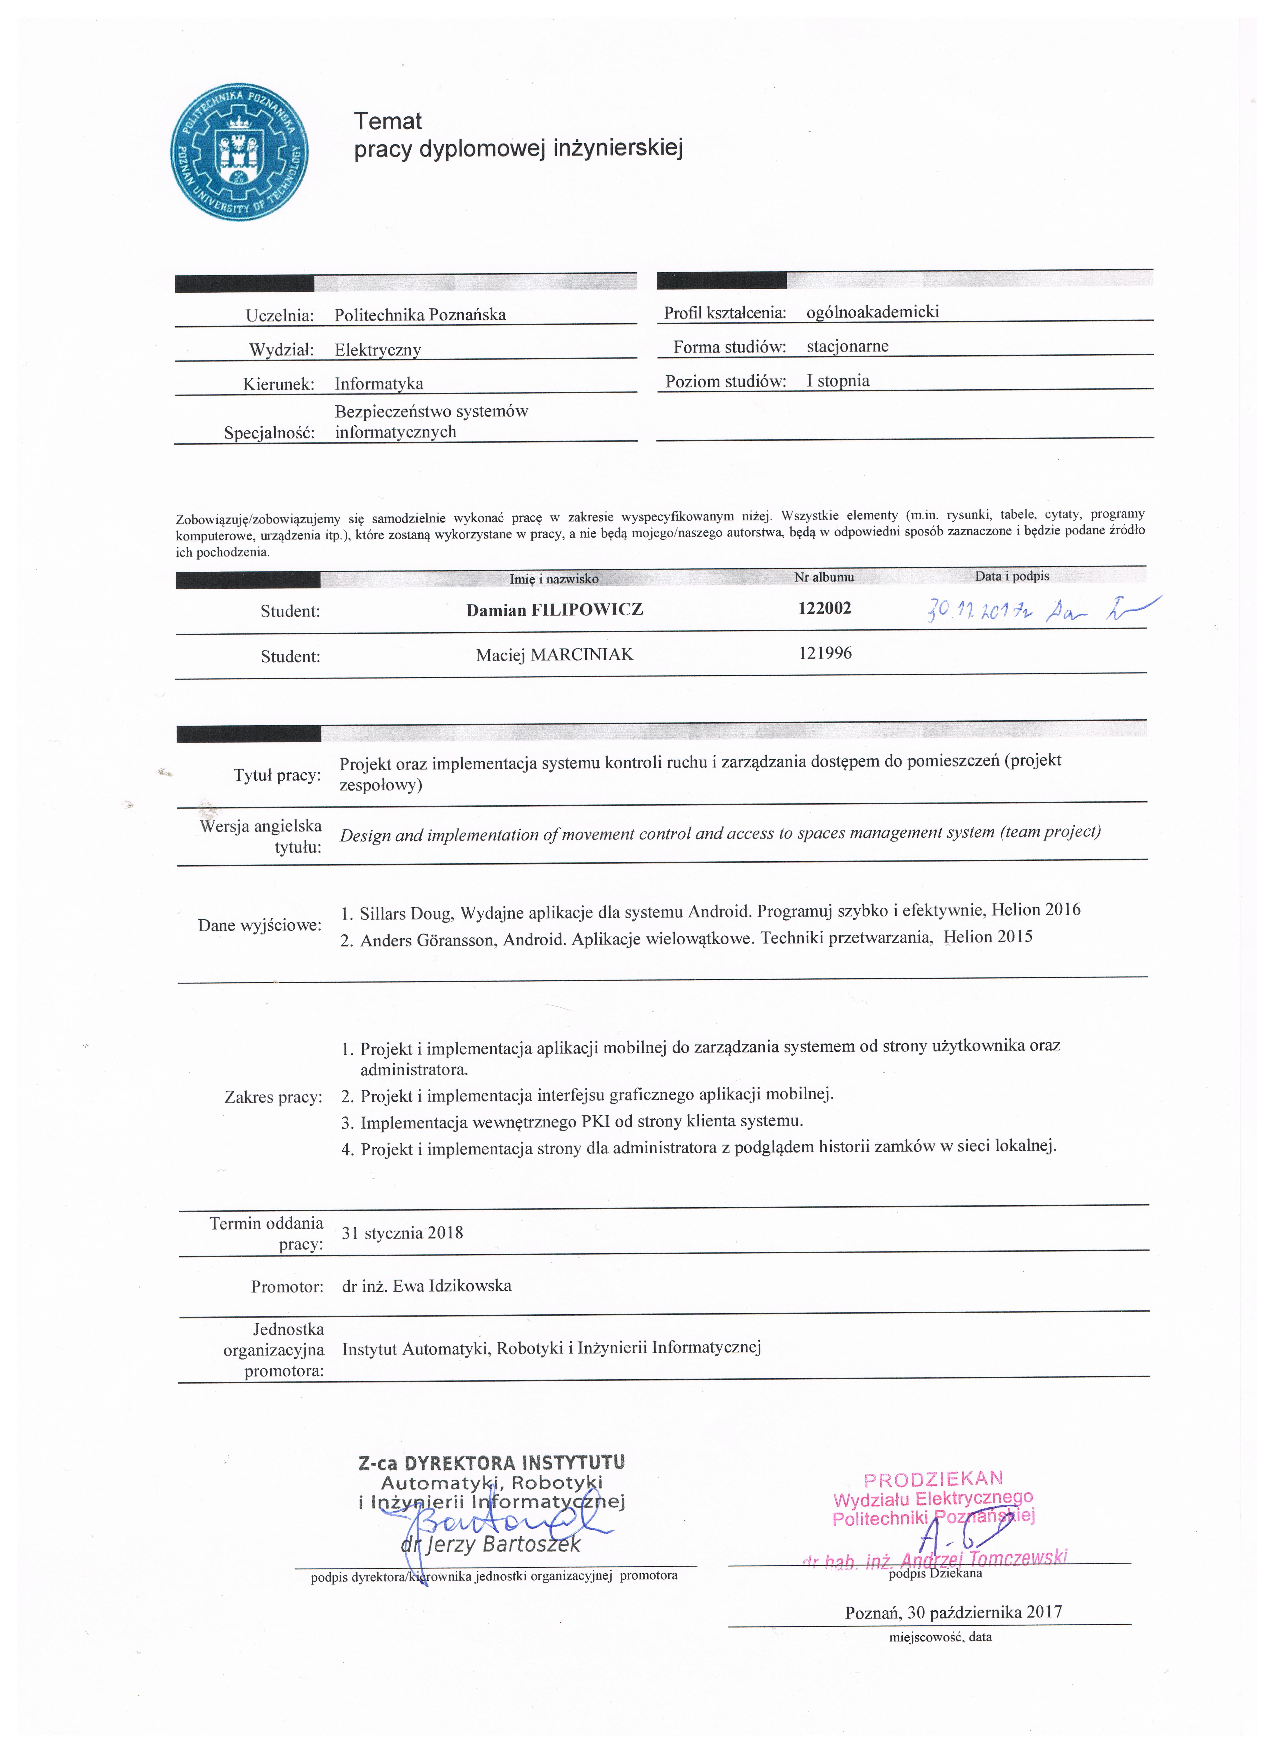
\includegraphics[width=13.2cm]{Obrazy/Karta_pracy_Damian}
\newpage
\textit{karta pracy umieszczona tylko informacyjnie}

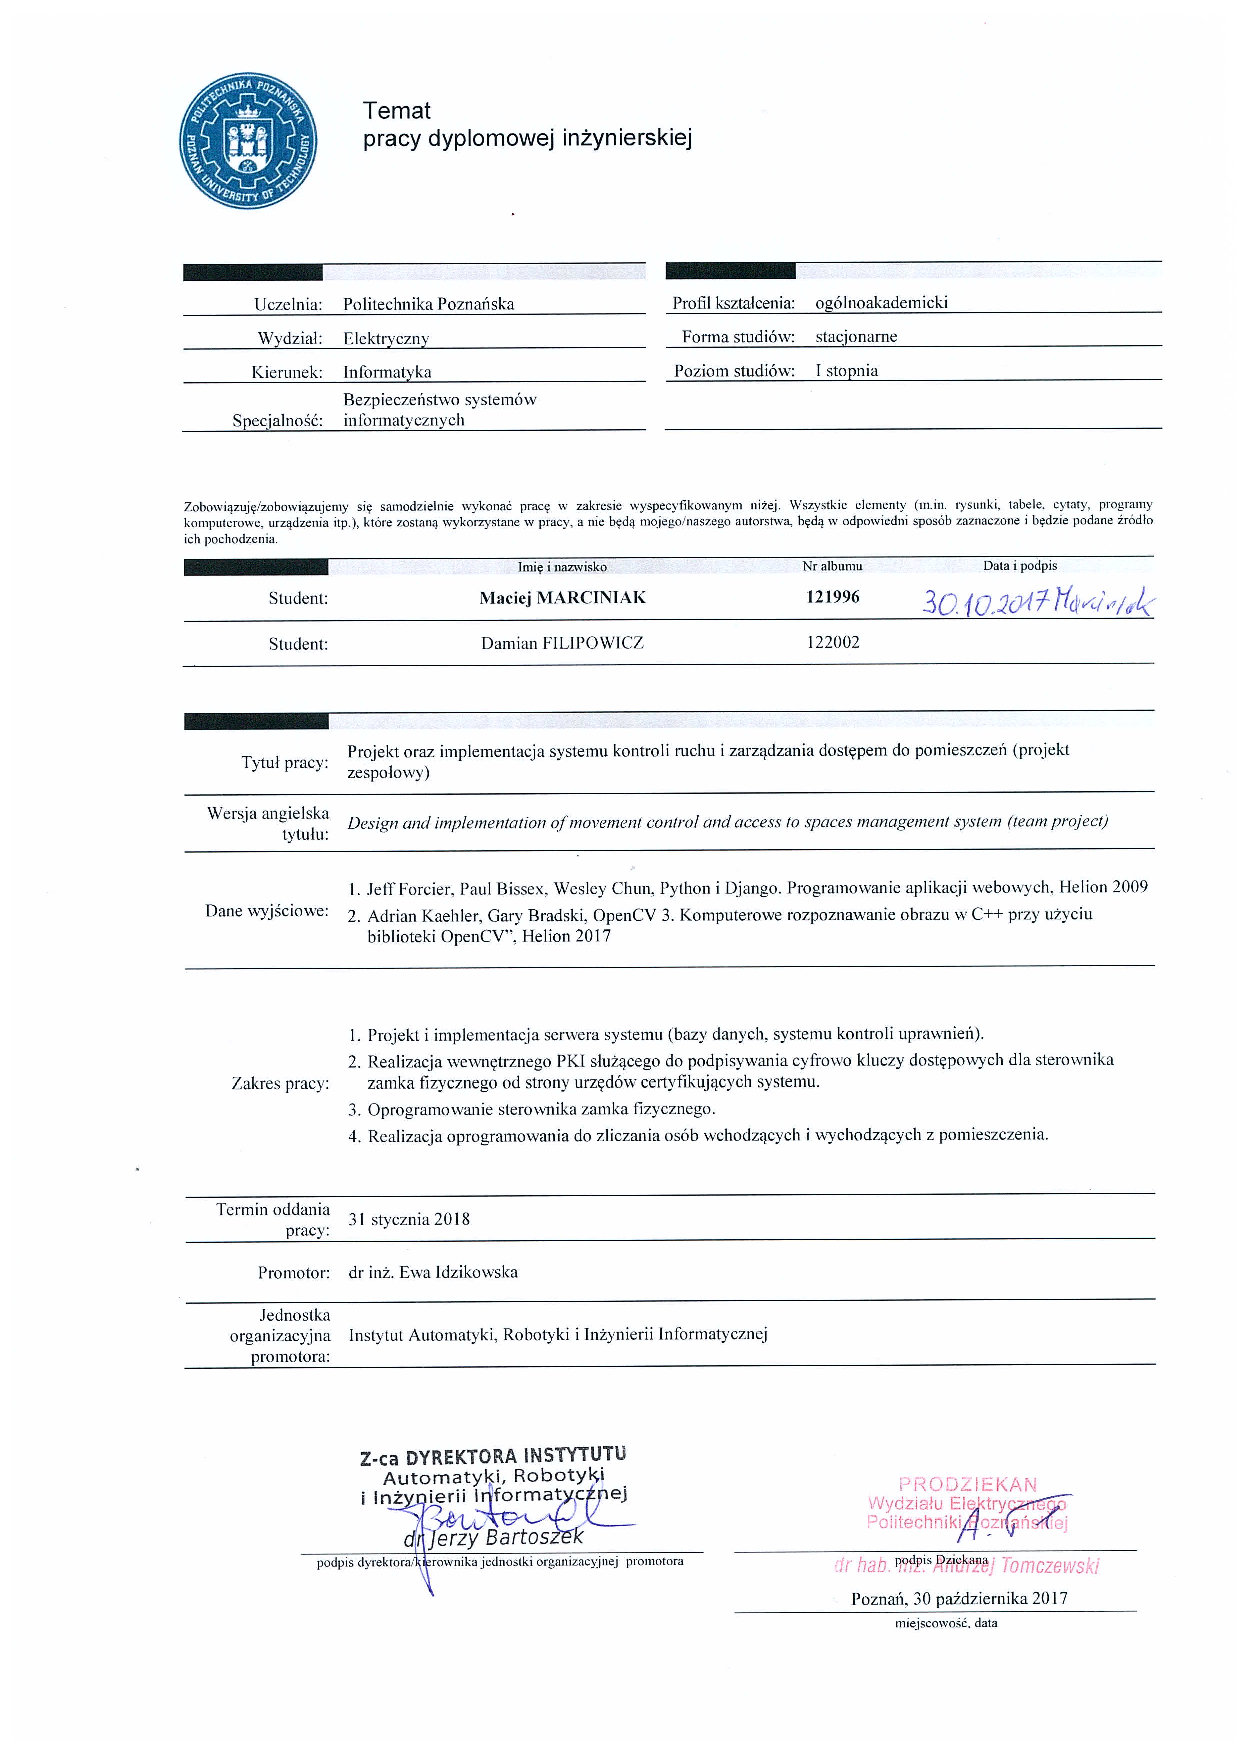
\includegraphics[width=13.2cm]{Obrazy/Karta_pracy_Maciej}

\newpage
\thispagestyle{empty}
\begin{center}
Poznan University of Technology\\
Faculty of Electrical Engineering\\
Institute of Control, Robotics and Information Engineering\\
\vspace{20mm}
\huge{\TytulAngielski} \\
\Large{by}\\
\vspace{5mm}
\Large{\StudentA}\\
\Large{\StudentB}\\
\vspace{20mm}

\normalsize\textbf{Abstract} \\
{Thesis presents the design and implementation of a traffic control system and room access management. \linebreak The basic assumption is to supervise the opening and closing of doors in the area of a large building where there are many entrances. The system stores data about users and their access rights, when and where they can enter. This information can be found in the MySQL database located on the server. The presented effects of the system are divided into a mobile application with the Android system and a website. The remaining part of the system (control devices, server) perform logic functions in the system, they connect strictly program modules between them. The virtual part of the system is based on Python 2.7 and Django.} 

\end{center}

\begin{center}
\textbf{Streszczenie} \\
{Praca dyplomowa przedstawia projekt i wykonanie systemu kontroli ruchu i zarządzania dostępem do~pomieszczeń. Podstawowym założeniem jest nadzorowanie, otwierania i zamykania drzwi w obrębię dużego budynku, gdzie znajduje się wiele wejść. System przechowuje dane na temat użytkowników oraz ich uprawnień dostępu, kiedy i gdzie mogą wchodzić. Informacje te znajdują się w bazie danych MySQL, umieszczonej na serwerze. Przedstawiane efekty działania systemu podzielone są na~aplikację mobilną z~system Android oraz stronę internetową. Pozostała część systemu (urządzenia sterujące, serwer), spełniają funkcje logiczne w~systemie, to znaczy łączą stricte programowo moduły pomiędzy sobą. Wirtualna część systemu oparta jest na~technologii Python 2.7 oraz Django.} 
\end{center}



\newpage\tableofcontents     % Spis tresci
\newpage\section{Wstęp}\label{sec:wstep}
Wstęp pracy zawiera krótki opis celu i zakresu planowanego projektu. System nosi potoczną nazwę \linebreak \NazwaSys, która związana jest z dodaniem  pewnych szczególnych funkcjonalności względnie zwykłym przedmiotom, tak~jak~dzieje się to w obecnie modnych urządzeniach\cite{porownanie zamkow} typu Internet of Things. Znaczna część znajdujących się na rynku rozwiązań dedykowana jest użytkownikom indywidualnym, do użytku domowego, natomiast opisywany system przeznaczony jest do zastosowań biurowych (dla średnich i dużych przedsiębiorstw).

Praca wykonywana jest zespołowo i w celu oznaczenia fragmentów, za które jest odpowiedzialna dana osoba, przybrano następujący format zapisu: w  tytułach fragmentów widnieje w nawiasach kwadratowych imię oraz nazwisko osoby wykonującej dany fragment. W przypadku, kiedy~nie~ma nawiasów oznacza to, że fragment został opracowany wspólnie.

Podział prac wygląda następująco:
\begin{itemize*}
\item Maciej Marciniak:
\begin{enumerate*}
\item Stworzenie oprogramowania do zliczania osób, wchodzących i wychodzących z pomieszczenia,
\item Implementacja serwera systemu (bazy danych, systemu kontroli uprawnień),
\item Utworzenie wewnętrznego PKI, służącego do podpisywania cyfrowo kluczy dostępowych dla sterownika zamka fizycznego od strony urzędów certyfikujących systemu,
\item Oprogramowanie sterownika zamka fizycznego.
\end{enumerate*}
\item Damian Filipowicz:
\begin{enumerate*}
\item Zaprojektowanie oraz stworzenie graficznego interfejsu aplikacji mobilnej,
\item Implementacja wewnętrznego PKI od strony klienta systemu,
\item Stworzenie oprogramowania do aplikacji mobilnej do zarządzania systemem (od strony użytkownika oraz administratora),
\item Utworzenie strony dla administratora z podglądem historii zamków w sieci lokalnej.
\end{enumerate*}
\end{itemize*}

\subsection{Cel i zakres pracy}

Celem pracy jest projekt i implementacja systemu kontroli ruchu oraz zarządzania dostępem do pomieszczeń. System ma na celu zamianę sposobu zarządzania dostępem w budynkach ze starszymi modelami, opartymi na fizycznych zamkach z kluczami fizycznymi, bądź systemów, opartych na kartach magnetycznych na system posługujący się urządzeniami mobilnymi z systemem operacyjnym Android. Głównym celem jest usprawnienie uzyskiwania  dostępu do pomieszczeń, dzięki wyeliminowaniu konieczności posiadania przy sobie wielu kluczy fizycznych oraz sytuacji, w których użytkownik zapomniałby klucza lub karty magnetycznej i nie mógłby uzyskać dostępu. Rozwiązaniem tych problemów jest możliwość przenoszenia kluczy (uprawnień) między telefonami. 
Dodatkowo nasz projekt ma usprawniać takie elementy, jak zarządzanie dostępem do wielu pomieszczeń oraz kontrolę osób, przebywających w danym pomieszczeniu poprzez moduł zliczania osób wchodzących i wychodzących.

W kwestii bezpieczeństwa systemu, naszym zadaniem było spełnienie wymagań dotyczących zabezpieczeń systemu, poprzez zastosowanie szeregu funkcji kryptograficznych przy procesie uwierzytelniania, jak i przy generowaniu kluczy takich jak np. funkcje skrótu, SSH, algorytmów szyfrowania asymetrycznego oraz zastosowania infrastruktury klucza publicznego.

Zakres pracy w tworzeniu projektu oraz implementacji, obejmował takie elementy, jak zaprojektowanie oraz stworzenie aplikacji klienckiej i serwerowej, oprogramowania do zliczania osób w pomieszczeniu, oprogramowania służącego do nadzorowania fizycznego dostępu do pomieszczenia, jak również strony internetowej, jako panel administracyjny administratora systemu.

\newpage
\subsection{Plan pracy}
Praca w pierwszej kolejności przedstawia dziedzinę projektu, której dotyczy. Poniżej zostaną wyjaśnione używane pojęcia oraz nazwy własne, umożliwiające poprawną interpretację opisanych działań. Po objaśnieniu terminologii, nasz projekt zostanie porównany z istniejącymi rozwiązaniami podobnego typu oraz zostaną sformułowane wnioski na temat niedopracowania lub możliwości poprawy danych rozwiązań, jakie zastosowano projektując opisywany w pracy system. Na zakończenie prezentacji dziedziny, zostanie opisany stan wykonania pracy w ramach zajęć przedmiotowych w trakcie trwania studiów inżynierskich.

Następny rozdział ma na celu przedstawienie ogólnego zarysu systemu. Opisany zostanie schemat połączeń poszczególnych modułów, interfejsów komunikacyjnych oraz wykaz wszystkich elementów składowych, wraz z możliwymi użytkownikami.

Czwarty rozdział dotyczy przybliżenia użytych technologii wraz z uzasadnieniem. Opis wyszczególnia zastosowane narzędzia do implementacji każdego~z~modułów oraz narzędzia umożliwiające pracę zespołową.

Główny rozdział pracy dotyczy projektu systemu. Zostały tutaj w pierwszej kolejności opisane diagramy UML (przypadków użycia, bazy danych oraz klas), które są odzwierciedleniem dalszej implementacji. Następnie przybliżony został uproszczony schemat elektryczny urządzenia sterującego zamkiem fizycznym oraz moduł zliczający ludzi. Kolejne punkty opisują szczegółowo komunikację pomiędzy urządzeniami oraz interfejs graficzny aplikacji mobilnej ~i~strony internetowej. Na zakończenie opisu projektu zostaną przybliżone dokładniej zaprojektowane mechanizmy zapewniające bezpieczeństwo ze~względu na~podstawowe zasady: poufność, dostępność i integralność.

Po omówieniu projektu, zostanie opisana implementacja systemu. Dział ten przybliży wybrane, kluczowe fragmenty programów oraz dokładniej określi metodykę powstałego kodu. 

Następny dział pracy skupi się na bezpieczeństwie systemu. Omówione zostaną szczegółowo zastosowane metody kryptograficzne oraz zostanie przeprowadzona analiza pod względem listy najczęstszych podatności OWASP Top 10. W podsumowaniu działu, zostaną zaproponowane możliwości poprawy  bezpieczeństwa systemu, których nie uwzględniono w fazie projektu, ani potem w implementacji.

W końcowej części pracy zawarte jest omówienie przeprowadzanych testów pod względem poprawności działania systemu. Jednocześnie zostanie graficznie przedstawione działanie każdego modułu.

\subsection{Metodyka pracy grupowej}
Metodyka użyta podczas pracy grupowej była oparta o model kaskadowy, składający się z etapów takich jak:
\begin{itemize*}
\item Planowanie systemu,
\item Analiza systemu,
\item Projekt systemu,
\item Implementacja,
\item Testowanie,
\item Wdrożenie i pielęgnacja produktu.
\end{itemize*}

Uzasadnieniem wyboru wyżej wymienionej metodyki, jest fakt popularności stosowania podczas realizowania dużych projektów inżynierskich. Kolejnym argumentem przy wyborze tej metodyki jest brak konieczności pokazywania fragmentów, działającego systemu podczas tworzenia pracy inżynierskiej. W~początkowej fazie priorytetem było określenie specyfiki wymagań systemu oraz zaprojektowanie, w dalszej kolejności implementacja systemu\cite{waterfall}.

\newpage
\section{Opis dziedziny przedmiotowej pracy}\label{sec:dziedzina}
Rozdział poniższy zawierać będzie objaśnienia używanych zwrotów i pojęć, umożliwiających poprawne interpretowanie dalszych tekstów. Następnie opisany zostanie stan wiedzy, związanej z tematyką pracy, to znaczy omówienie wybranych rozwiązań systemów, tak zwanych inteligentnych zamków. W zestawieniu porównane zostaną również zaproponowane w pracy dyplomowej rozwiązania.
\subsection{Pojęcia i definicje}\label{sec:Pojęcia i definicje}
W poniższej pracy inżynierskiej posługiwać się będziemy następującymi pojęciami:
\begin{itemize*}
\item {Klucz dostępowy} --- jest to  klucz określający dostęp do pomieszczenia dla~użytkownika w konkretnych dniach oraz godzinach,
\item {Klucz szyfrujący} 
--- jest to klucz prywatny \footnote{ klucz prywatny szerzej został opisany w rozdziale \ref{sec:Projekt PKI}}, wygenerowany podczas tworzenia certyfikatu klucza szyfrującego. Używany jest on do szyfrowania wiadomości, wysyłanej z aplikacji mobilnej do urządzenia sterującego,
\item {Klucz deszyfrujący }
--- jest to klucz publiczny \footnote{ klucz publiczny szerzej został opisany w rozdziale \ref{sec:Projekt PKI}}, wygenerowany podczas tworzenia certyfikatu klucza szyfrującego. Używane jest on do odszyfrowania wiadomości, wysyłanej z aplikacji mobilnej do urządzenia sterującego,
\item {Inteligentny zamek}
--- system obsługujący otwieranie elektrozamka bądź serwomechanizmu,
\item {Konto}
--- reprezentacja użytkownika w systemie za pomocą takich danych, jak login hasło, imię, nazwisko.
\item {Administrator}
--- jest to fizyczna osoba, posiadającą dla swojego konta uprawnienia administratora, co wiąże się z pełnym dostępem do systemu,
\item {Certyfikat dostępowy}
--- jest to certyfikat przechowujący informacje, takie jak dane użytkownika, do jakiego pomieszczenia oraz w jakich dniach i~godzinach~ma dostęp
\item {Certyfikat klucza szyfrującego}
-- jest to certyfikat przechowujący dane o~użytkowniku, ważności klucza szyfrującego oraz sam klucz deszyfrujący.
\end{itemize*}

\subsection{Stan wiedzy}\label{sec:Stan wiedzy}
Przed przystąpieniem do projektu, wykonaliśmy rozeznanie w działu systemów zbliżonych do naszego, które na dany moment funkcjonowały na rynku. Po~tej analizie doszliśmy do wniosku, że wszystkie poznane przez nas systemy inteligentnych zamków wykonane przez uznane firmy, takie jak Gerda Lock, czy Danalock, zostały wykonane typowo dla użytku domowego, a nie tak jak zakłada nasz projekt inżynierski, z  przeznaczeniem do zarządzania w budynkach o większej złożoności, takich jak biurowce, z różnym stopniem dostępu. Opis wraz z porównaniem poszczególnych systemów, znajduje się w tabelach poniżej.

Tabela \ref{tab:porownanie1} zawiera porównanie firm pod względem otwierania zamka. Już w pierwszym wierszu tabeli można zauważyć indywidualny charakter zastosowania systemów, ponieważ każdy z prezentowanych systemów, poza firmą August, nie~oferuje obsługi wielu urządzeń z poziomu jednej aplikacji. Proponowane przez nas~rozwiązanie umożliwia skalowalność systemu oraz wprowadzanie różnorodności w~zarządzaniu dostępem. Następne funkcjonalności wprowadzają zagrożenia lub zwiększają podatności sytemu na ataki hakerskie. Na przykład otwieranie każdego zamka z dowolnego miejsce przez stronę WWW, daje możliwość zdalnego sterowania dostępem w całym systemie. Skutkuje to brakiem kontroli, czego efektem może być zagrożenie uzyskania dostępu przez nieuprawnione osoby.
\newpage
\begin{longtable}[!ht]{|m{5cm}|m{1.5cm}|m{1.6cm}|m{1.9cm}|m{2cm}|m{2cm}|} 
\caption{Tabela porównania otwierania zamków}
\label{tab:porownanie1}\\
\hline
Funkcja & NUKI\cite{NUKI} & August\cite{August} & DanaLock\cite{DanaLock} &
Gerda Lock\cite{GerdaLock} & 
Nasz system  \\ \hline
Zarządzanie wieloma zamkami z jednej aplikacji
& brak & tak & brak & brak & tak \\ \hline
Otwieranie zamka przy pomocy strony WWW
& brak & brak & tak & brak & brak \\ \hline
Inne sposoby otwarcia zamka niż aplikacja
& brak & brak & brak & tak & tak \\ \hline
Automatyczne zamykanie zamka
& brak & tak & tak & tak & tak \\ \hline
Tryb otwierania zamka automatycznie
& tak& brak & tak & tak & nie \\ \hline
Tryb otwierania zamka po zezwoleniu przyciskiem
& brak & tak & tak & tak & tak \\ \hline
\end{longtable}

Tabela \ref{tab:porownanie2} zawiera porównanie firm pod względem zasilania i montażu. Wszystkie systemy zawierały podstawowe wady eksploatacyjne, gdy system w~budynku zawierałby wiele urządzeń danego typu, to znaczy problem z zasilaniem. Nasz system oferuje podłączenie zasilania bezpośrednio z sieci, taka konfiguracja pozwala uodpornić system na konieczność wymiany baterii w każdym zamku. Gdyby jednak konieczne było zasilanie awaryjne, w sytuacji zaniku napięcia, możliwe jest zastosowanie UPSów, które podtrzymają urządzenia przez czas awarii.
\begin{longtable}[!ht]{|m{5cm}|m{1.7cm}|m{1.7cm}|m{1.7cm}|m{2cm}|m{2.4cm}|} 
\caption{Tabela porównania zasilania i montażu}
\label{tab:porownanie2}\\
\hline
Funkcja & NUKI & August &DanaLock & Gerda Lock & Nasz system \\ \hline
Zasilanie zewnętrzne (z sieci)
& brak & brak & brak & brak & tak \\ \hline
Zasilanie bateryjne \newline (podstawowe/ awaryjne)
& podstawowe & podstawowe &podstawowe & podstawowe & możliwe \newline awaryjne \\ \hline
Sposób montażu
& nakładka na \linebreak zamek & nakładka na \linebreak zamek & nakładka na \linebreak zamek & nakładka na \linebreak zamek & nakładka na \newline zamek lub  \newline elektrozamek  \\\hline
\end{longtable}

Tabela \ref{tab:porownanie3} zawiera porównanie firm pod względem dziennika zdarzeń oraz powiadomień. Funkcjonalność naszego systemu zgodna jest z możliwościami firm NUKI oraz Gerda Lock. Pozostali dystrybutorzy nie udostępniają tak szczegółowych informacji na temat działania urządzeń.
\begin{longtable}[!ht]{|m{6cm}|m{1.4cm}|m{1.4cm}|m{1.7cm}|m{2cm}|m{2cm}|} 
\caption{Tabela porównania powiadomień działania}
\label{tab:porownanie3}\\
\hline
& NUKI & August & DanaLock & Gerda Lock & Nasz system \\ \hline
podgląd kto otworzył zamek
& taki & brak & brak & tak & tak \\ \hline
powiadomienie o otwarciu drzwi \newline (ogólnie i przez daną osobę)
& brak & brak & brak & tak & tak  \\ \hline
powiadomienie o nieautoryzowanych próbach otwarcia
& tak & brak & brak & tak & tak  \\ \hline
\end{longtable}

\newpage
\subsection{Stan pracy wykonany w ramach zajęć przedmiotowych} \label{sec:Stan pracy wykonany w ramach zajęć przedmiotowych}
W ramach zajęć projektowych oraz laboratoryjnych o nazwie \textit{Projekt Zespołowy}, prowadzonych \linebreak z~mgr.~Michałem Apolinarskim oraz dr Ewą Idzikowską, zostały wykonane następujące fragmenty systemu:

Aplikacja mobilna została wykonana dla wersji Androida minimum 4.4 KitKat w stopniu umożliwiającym podstawowe funkcjonalności, takie jak:
\begin{itemize*}
\item Logowanie użytkowników,
\item Rejestracja użytkowników,
\item Rejestracja wraz z tworzeniem certyfikatu klucza szyfrującego,
\item Generowanie nowego certyfikatu,
\item Pobieranie certyfikatów z serwera,
\item Zarządzanie certyfikatami użytkownika,
\item Zarządzanie prośbami o rejestracje,
\item Wnioskowanie o certyfikat nowy.
\end{itemize*}

Dodatkowo zostały zaimplementowane gniazdka sieciowe do obsługi połączenia bluetooth oraz w każdym widoku, który korzystał z połączenia z serwerem, były napisane fragmenty kodu. Funkcje te oraz kod zostały napisane bez~uwzględnienia wzorców architektonicznych (wszystko dotyczące danego widoku było zawarte w~jednej klasie) oraz posiadały szereg błędów powodujących niestabilne działanie systemu, a także stosowały metody z~systemu Android, które były określane przez środowisko Android Studio, jako ''deprecated''\footnote{ Jeśli funkcja jest oznaczona, jako deprecated to jest to informacja o tym, żę dana funkcja jest już przestarzała i może w nowszych modelach telefonów (dla nowszych systemów Android) nie działać}. Z racji pisania aplikacji dedykowanej dla systemu Android 4.4, wygląd różni się od tego, który został zaimplementowany w pracy inżynierskiej.

Aplikacja serwerowa została wykonana w stopniu umożliwiającym podstawowe funkcje, pozwalające na~komunikację pomiędzy urządzeniami. Api zapewniało w minimalnym stopniu bezpieczeństwo. 

Funkcje serwera utworzone w ramach zajęć przedmiotowych:
\begin{itemize*}
\item Logowanie użytkowników,
\item Rejestracja użytkowników,
\item Zapisywanie nowego certyfikatu dostępu,
\item Udostępnianie certyfikatów dostępowych,
\item Pobieranie list certyfikatów, próśb o certyfikaty oraz rejestracji.
\end{itemize*}

Wszystkie te funkcje zwracały odpowiednio pożądane dane, albo wartość ''Invalid'', co powodowało wyświetlanie komunikatów o błędach użytkownikowi bez rozróżniania powodu, np. awarii serwera (mylnie wysyłany komunikat ''Invalid'' zamiast komunikatu HTTP typu 500).

Urządzenie sterujące zamkiem zostało napisane w języku Python i pozwalało na odbieranie danych z~aplikacji mobilnej oraz posiadało funkcje odpowiedzialną za otwieranie zamka.

W ramach przedmiotu ochrona danych, prowadzonego przez dr inż. Anne Grocholewską-Czuryło, zostały zaimplementowane w systemie fragmenty PKI, takie jak:
\begin{itemize*}
\item Format certyfikatu klucza szyfrującego,
\item Generowanie nowego certyfikatu szyfrującego użytkownika,
\item Blokowanie użytkowników oraz certyfikatów szyfrujących systemu.
\end{itemize*}

Funkcje te zostały napisane zarówno po stronie aplikacji mobilnej jak~i~Aplikacji, serwerowej. Ponadto po~stronie androida został opracowany sposób przechowywania klucza prywatnego w formie zaszyfrowanego pliku hasłem użytkownika.

\newpage\section{Zarys idei systemu \textsl{\NazwaSys}}\label{sec:ideasystemu}
W rozdziale zostanie opisana pokrótce idea systemu \NazwaSys. Projekt składa się z 5 składowych: urządzenia sterującego (zarządzającego otwieraniem /zamykaniem drzwi), modułu zliczającego osoby, aplikacji mobilnej dedykowanej dla systemu Android oraz serwera operującego na bazie danych. Każdy z podsystemów zostanie przedstawiony, w jaki sposób ma funkcjonować, aby przybliżyć działanie systemu względem poszczególnych aktorów systemu (użytkowników, urządzeń).

\subsection{Schemat ideowy systemu \textsl{\NazwaSys}}
System łączy ze sobą 5 podsystemów różnymi interfejsami komunikacyjnymi.Urządzenia mobilne komunikują się z urządzeniem sterującym poprzez protokół bluetooth, a pozostałe połączenia oparte są na Ethernecie. Schemat połączeń urządzeń znajduje się na Rys. \ref{Schemat ogólny systemu}.

\begin{figure}[!h]
\centering
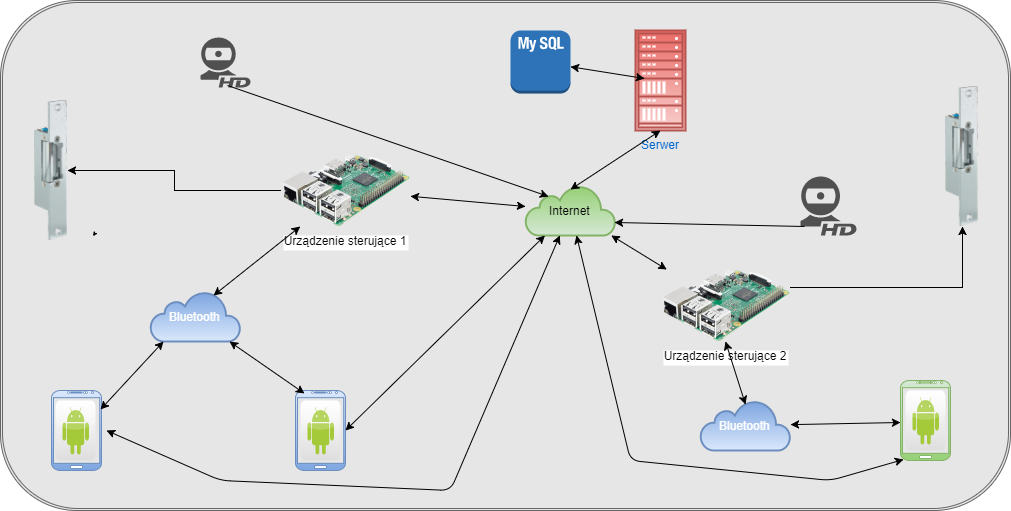
\includegraphics[width=15cm]{Obrazy/Schemat_ogolny}
\caption{Schemat ogólny systemu}
\label{Schemat ogólny systemu}
\end{figure}

Urządzenia sterujące łączą się z elektrozamkiem lub serwomechanizmem poprzez przewody elektryczne, natomiast z~kamerą IP oraz serwerem poprzez sieć LAN. Aplikacja serwerowa nawiązuje połączenie z bazą danych przez lokalny interfejs sieciowy.

\subsection{Opis składowych systemu}
System ma złożoną budowę, ponieważ składa się z 5 podsystemów. Pierwszym z nich jest urządzenie sterujące, w którego skład wchodzą Raspberry Pi~3\footnote{ Raspberry Pi 3 jest mikrokomputerem z procesorem ARMv7} oraz serwomechanizm lub zamek elektroniczny. Podstawową funkcją tego modułu jest weryfikacja klucza cyfrowego, przesyłanego przez urządzenia mobilne oraz otwieranie zamka przy pozytywnym wyniku weryfikacji. Każde zdarzenie zapisywane jest w pliku z logami. Oprogramowanie mikrokomputera obejmuje system Linux raspbian-jessie \footnote{ System operacyjny raspbian-jessie jest dedykowanym systemem operacyjnym dla komputerów Raspberry Pi umożliwiającym w pełni wykorzystać interfejsy wejścia wyjścia} oraz skrypt napisany w języku Python 2.7. Programy łączą się do serwera w celu pobrania informacji o poprawności i~dacie ważności certyfikatu dostępowego, następnie dane są porównywane z~tymi otrzymanymi od użytkownika. Dodatkowo weryfikowany jest podpis cyfrowy, którym sygnowany jest klucz dostępowy. Jeśli dane zostaną zweryfikowane poprawnie, to zostaje wysterowany serwomechanizm (lub wysłany impuls do elektrozamka), który otwiera zamek. W przeciwnym przypadku użytkownik zostanie poinformowany o odmowie dostępu, a nieudana próba dostania się do~systemu zarejestrowana zostanie w bazie danych wraz z danymi właściciela klucza dostępowego.

Drugim elementem jest aplikacja mobilna napisana na platformę Android w wersji minimalnej 5.0. Program ma na celu przechowywanie w pamięci smartphona kluczy cyfrowych (dostępowych) użytkownika oraz umożliwienie interakcji użytkownika z systemem.

Kolejnym z elementów jest aplikacja serwerowa wraz ze stroną internetową. Rolą serwera w tym systemie jest pośredniczenie w operacjach na danych dostępowych w bazie danych MySQL. Dodatkowo serwer obsługuje stronę internetową, która wyświetla na bieżąco historię użycia zamków w systemie.

Przedostatnim elementem składowym systemu jest baza danych, która przechowuje wszystkie kluczowe informacje systemu oraz udostępnia je serwerowi.

Ostatnim ze składowych systemu jest oprogramowanie zliczające liczbę osób wchodzących i wychodzących dla danego pomieszczeniu lub całego budynku wraz z kamerą, której zadaniem jest obliczanie informacji o~aktualnej liczbie osób w danym pomieszczeniu. 

\subsection{Podmioty systemu} 
W pracy dyplomowej można wyodrębnić następujące podmioty:
\begin{itemize}
\item {Użytkownik niezalogowany} --- jest to użytkownik, który posiada aplikacje mobilną na swoim urządzeniu, lecz nie wykonał procesu logowania,
\item {Użytkownik niezarejestrowany} --- jest to użytkownik który wysłał prośbę o zarejestrowanie, lecz nie została ona jeszcze zatwierdzona przez administratora,
\item {Użytkownik zalogowany} --- jest to użytkownik, który przeszedł poprawnie proces logowania, posiada on ograniczoną funkcjonalność aplikacji,
\item {Administrator} --- jest to użytkownik zalogowany, który posiada uprawnienia administratora, co wiąże się z pełnym dostępem do funkcji aplikacji mobilnej (zawiera funkcje użytkownika zalogowanego),
\item {Aplikacja serwerowa} --- jest to oprogramowanie, zarządzające całym systemem oraz pośredniczące w przekazywaniu informacji z bazy danych,
\item {Urządzenie sterujące} --- jest to oprogramowanie zarządzające dostępem fizycznym do pomieszczeń,
\item {Elektrozamek} --- urządzenie umieszczone w futrynie drzwi, pozwalające sterować stanem otwarcia zamka,
\item {Serwomechanizm} --- silnik krokowy, nakładka na zamek fizyczny w drzwiach, sterujący ryglem w futrynie,
\item {Moduł zliczania osób} --- jest to oprogramowanie zwracające w czasie rzeczywistym ilość osób przebywających w danym pomieszczeniu,
\item {Kamera IP} --- urządzenie wizyjne, udostępniające obraz do celów zliczania osób.
\end{itemize}

\newpage\section{Wybór technologii informatycznych} \label{sec:technologie}
Prezentowany projekt ze względu na rozbudowaną konstrukcję, składa się również z wielu technologii informatycznych. Dominującymi językami programowania są Python oraz Java (z elementami języka Kotlin). Wybór oraz uzasadnienie decyzji zostało przedstawione w poniższych punktach.

\subsection{Urządzenie sterujące [Maciej Marciniak]}
Urządzenie sterujące utworzone zostało na mikrokomputerze Raspberry Pi 3, ze względu na szereg interfejsów dostępnych na płytce. Inne rodzaju mikrokontrolery np. typy STM32 umożliwiają podłączenie takich urządzeń jak~bluetooth oraz karta sieciowa WiFi, lecz jest to wówczas zintegrowany układ (celem pracy dyplomowej nie było tworzenie płytki PCB pozwalającej zintegrować układy) oraz drugim powodem jest wydajność i~elastyczność programów. 

Podczas projektowania urządzenia sterującego zastosowano następujące technologie:
\begin{itemize*}
\item język programowania Python w wersji 2.7.13 wraz z bibliotekami PyCrypto\footnote{ Biblioteka udostępniająca funkcje kryptograficzne języka Python}, MySQL-db\footnote{ Biblioteka zawierająca interfejs obsługujący API do bazy MySQl} oraz BlueZ \footnote{ Biblioteka ułatwiająca zarządzanie modułem Bluetooth },
\item format zapisu danych JSON,
\item biblioteka RPI.GPIO
\footnote{ Biblioteka oferująca klasy do obsługi portów  wejścia/wyjścia dla języka Python}, aby uzyskać dostęp do interfejsu wejścia/wyjścia.
\end{itemize*}

Programem wykorzystywanym do implementacji programu jest PyCharm w wersji 2017.2.4. Wybór technologii oraz oprogramowania związany był z wysokim stopniem integracji urządzenia Raspberry Pi z językiem Python. Środowisko PyCharm zostało wybrane ze względu na zaawansowane funkcjonalności wspomagające tworzenie kodu o wysokiej czytelności oraz IDE udostępnia funkcję Inteli-sense (podpowiedzi pod względem wartości, pól klas, procedur).

\subsection{Aplikacja serwera i baza danych [Maciej Marciniak]}
Aplikacja serwerowa została stworzona przy pomocy środowiska programistycznego PyCharm w wersji 2017.1.4. Technologie użyte w aplikacji serwerowej były następujące:
\begin{itemize*}
\item język programowania Python w wersji 2.7.13 wraz z bibliotekami PyCrypto i MySQL-db,
\item framework Django,
\item baza danych MySQL wykorzystująca oprogramowanie XAMPP w celu emulacji środowiska Apache,
\item format zapisu danych JSON,
\item HTML5,
\item Bootstrap 3.
\end{itemize*}

Wybór wyżej wymienionych technologii uzasadniony jest popularnością serwisów Webowych, opartych o~framework Django, wskazuje na to liczna liczba ofert pracy względem innych frameworków. Z powodu zastosowania Django, zdecydowano jednocześnie o użyciu języka Python oraz bazy danych MySQL ze~względu na bardzo wysoką kompatybilność tych technologii. Html5 został wybrany ponieważ, jest to najnowsza wersja. Natomiast framework Bootstrap został wybrany z względu na intuicyjne tworzenie w nim stron responsoryjnych oraz dobrą współpracę z frameworkiem Django.

\newpage
\subsection{Aplikacja mobilna [Damian Filipowicz]}
Aplikacja mobilna została stworzona przy pomocy zintegrowanego środowiska programistycznego Android Studio w wersji 3.0 wraz z zintegrowanym emulatorem Genymotion z licencją darmową. "Srodowisko Android Studio w wersji 3.0 zostało wybrane ze względu na kompatybilność z językiem Kotlin oraz wsparcie oficjalne firmy Google \footnote{Firma Google obecnie jest odpowiedzialna za rozwój systemu operacyjnego Android.} dla tego środowiska . Zdecydowano się na~wybór systemu Android, ponieważ cieszy się bardzo dużą popularnością (urządzenia z systemem Windows są już dużą rzadkością). W przyszłości rozwoju projektu uwzględnić można również urządzenia z system iOS. Ze względu na~możliwości stosowania wielu języków programowania wewnątrz jednej aplikacji, użyto następujących technologii:
\begin{itemize*}
\item Java w wersji dla systemów Android jako podstawa funkcjonowania aplikacji,
\item Kotlin --- jako język poszerzający możliwości języka Java oraz pozwalający tworzyć kod o mniej objętości, tzn. bardziej czytelny,
\item XML ---język prezentowania grafiki w systemie Android. systemami,
\item JSON --- format zapisu danych.
\end{itemize*}

Cała aplikacja ponadto została napisana w oparciu o wzorzec architektoniczny MVP \footnote{ Wzorzec architektoniczny Model--View Presenter w którym View odpowiedzialny jest za generowanie widoków model przechowuje informacje o obiektach systemu natomiast presenter przechowuje całą logikę biznesową}. Zastosowano wyżej wymienione języki ze względu na wydajność programów w języku Java w systemach Android oraz chęci poznania nowego języka programowa Kotlin, który jest w pełni kompatybilny z językiem Java (przetwarzany do Javy).  

\subsection{Moduł zliczania osób [Maciej Marciniak]}
Moduł zliczania osób jest mocno związany z aplikacją urządzania sterującego ze względu na to, że zostaną uruchomione na jednym mikrokomputerze Raspberry Pi. Zastosowano zatem język Python w wersji 2.7.13 oraz bibliotekę graficzną Open-CV, dzięki któremu w łatwy sposób można przetwarzać obrazy zaawansowanymi metodami. 

\subsection{System kontroli wersji}
Podczas tworzenia prezentowanej pracy użyto systemu kontroli wersji GIT wraz z  oprogramowaniem desktopowym, przeznaczonym dla środowiska Windows o nazwie GitHub Desktop. Zastosowano takie oprogramowanie, ponieważ w znacznym stopniu ułatwia współbieżne tworzenie kodu programu oraz w czytelny sposób prezentuje wprowadzane zmiany pomiędzy iteracjami wersji udostępnianych programów. 

\subsection{Prowadzenie dokumentacji}
Dokumentacja pracy dyplomowej prowadzona została w języku LaTeX przy pomocy oprogramowania \linebreak TexStudio. Technologia wymaga większej pracy wejściowej, aby poprawnie sformatować tekst, lecz w przypadku potrzeby edycji poszczególnych fragmentów, pozwala zachować zaplanowany format w pozostałych fragmentach dokumentu. Język LaTeX umożliwia w szybki sposób zmianę formatu całego dokumenty (np. wielkości czcionki, stylu nagłówków bez potrzeby przetwarzania całego tekstu). Ponadto do tworzenia diagramów UML został wykorzystany program Visual Paradigm 14.2 oraz Inteli Idea 2017 Enterprise. Wybór pierwszego z nich był podyktowany dobrą znajomością tego środowiska, natomiast drugi został wybrany z względu na funkcję umożliwiającą wygenerowanie diagramów klas z gotowego kodu. W celu utworzenia dokumentacji elektrycznej, użyto programu KiCAD w wersji 4.0.6 ze względu na prostą obsługę i darmową licencję.
 
\newpage\section{Projekt systemu \textsl{\NazwaSys}}\label{sec:projekt}
Głównym celem pracy dyplomowej jest zaprojektowanie systemu. Opisywany rozdział dokładnie przedstawi projekt kompletnego systemu. Punkt \ref {sec:Diagramy UML} obrazuje na diagramach UML przypadki użycia poszczególnych funkcjonalności urządzeń, następnie wyszczególnione zostaną sekwencje działań głównych funkcji systemu oraz przedstawione zostaną modele bazy danych i wszystkich klas wyszczególnione dla każdego urządzenia osobno. 

Podrozdział \ref {sec:Schemat elektryczny zamka} zawiera uproszczony schemat elektryczny urządzenia sterującego zamkami. Następnie przedstawiona zostanie komunikacja modułów z aplikacją serwerową, tzn. opisane zostanie API serwera, pozwalające podłączenie innych urządzeń do systemu oraz przebieg transmisji danych pomiędzy urządzeniem sterującym a aplikacją mobilną.

Punkt \ref{sec:Projekt interfejsu graficznego} przedstawia projekt interfejsu graficznego wraz z objaśnieniami zastosowanej kolorystyki i~symboli.

Ostatni rozdział opisuje mechanizmy bezpieczeństwa, zaprojektowane w systemie, z uwzględnieniem głównych właściwości poufności, integralności oraz dostępności.

\subsection{Diagramy UML}\label{sec:Diagramy UML}
Podrozdział zawiera projekt systemu w postaci diagramów UML. W pierwszej kolejności przedstawiony zostanie diagram przypadków użycia, gdzie wymienione będą wszystkie funkcjonalności systemu oraz przyłączone do nich zostaną poszczególne podmioty (aktorzy) systemu, które biorą udział przy wykonywaniu danej funkcjonalności. Następnie omówiony zostanie diagram relacji oraz encji bazy danych. Na koniec omówione zostaną diagramy klas, wykonane dla każdego modułu osobno. 
\subsubsection{Diagram przypadków użycia [Maciej Marciniak]}
Diagram przypadków użycia (funkcjonalności) systemu wraz z odpowiadającymi aktorami przedstawiono na Rys. \ref{diagram:diagram przypadków_użycia}.
\begin{landscape}
\begin{figure}[!h]
\centering
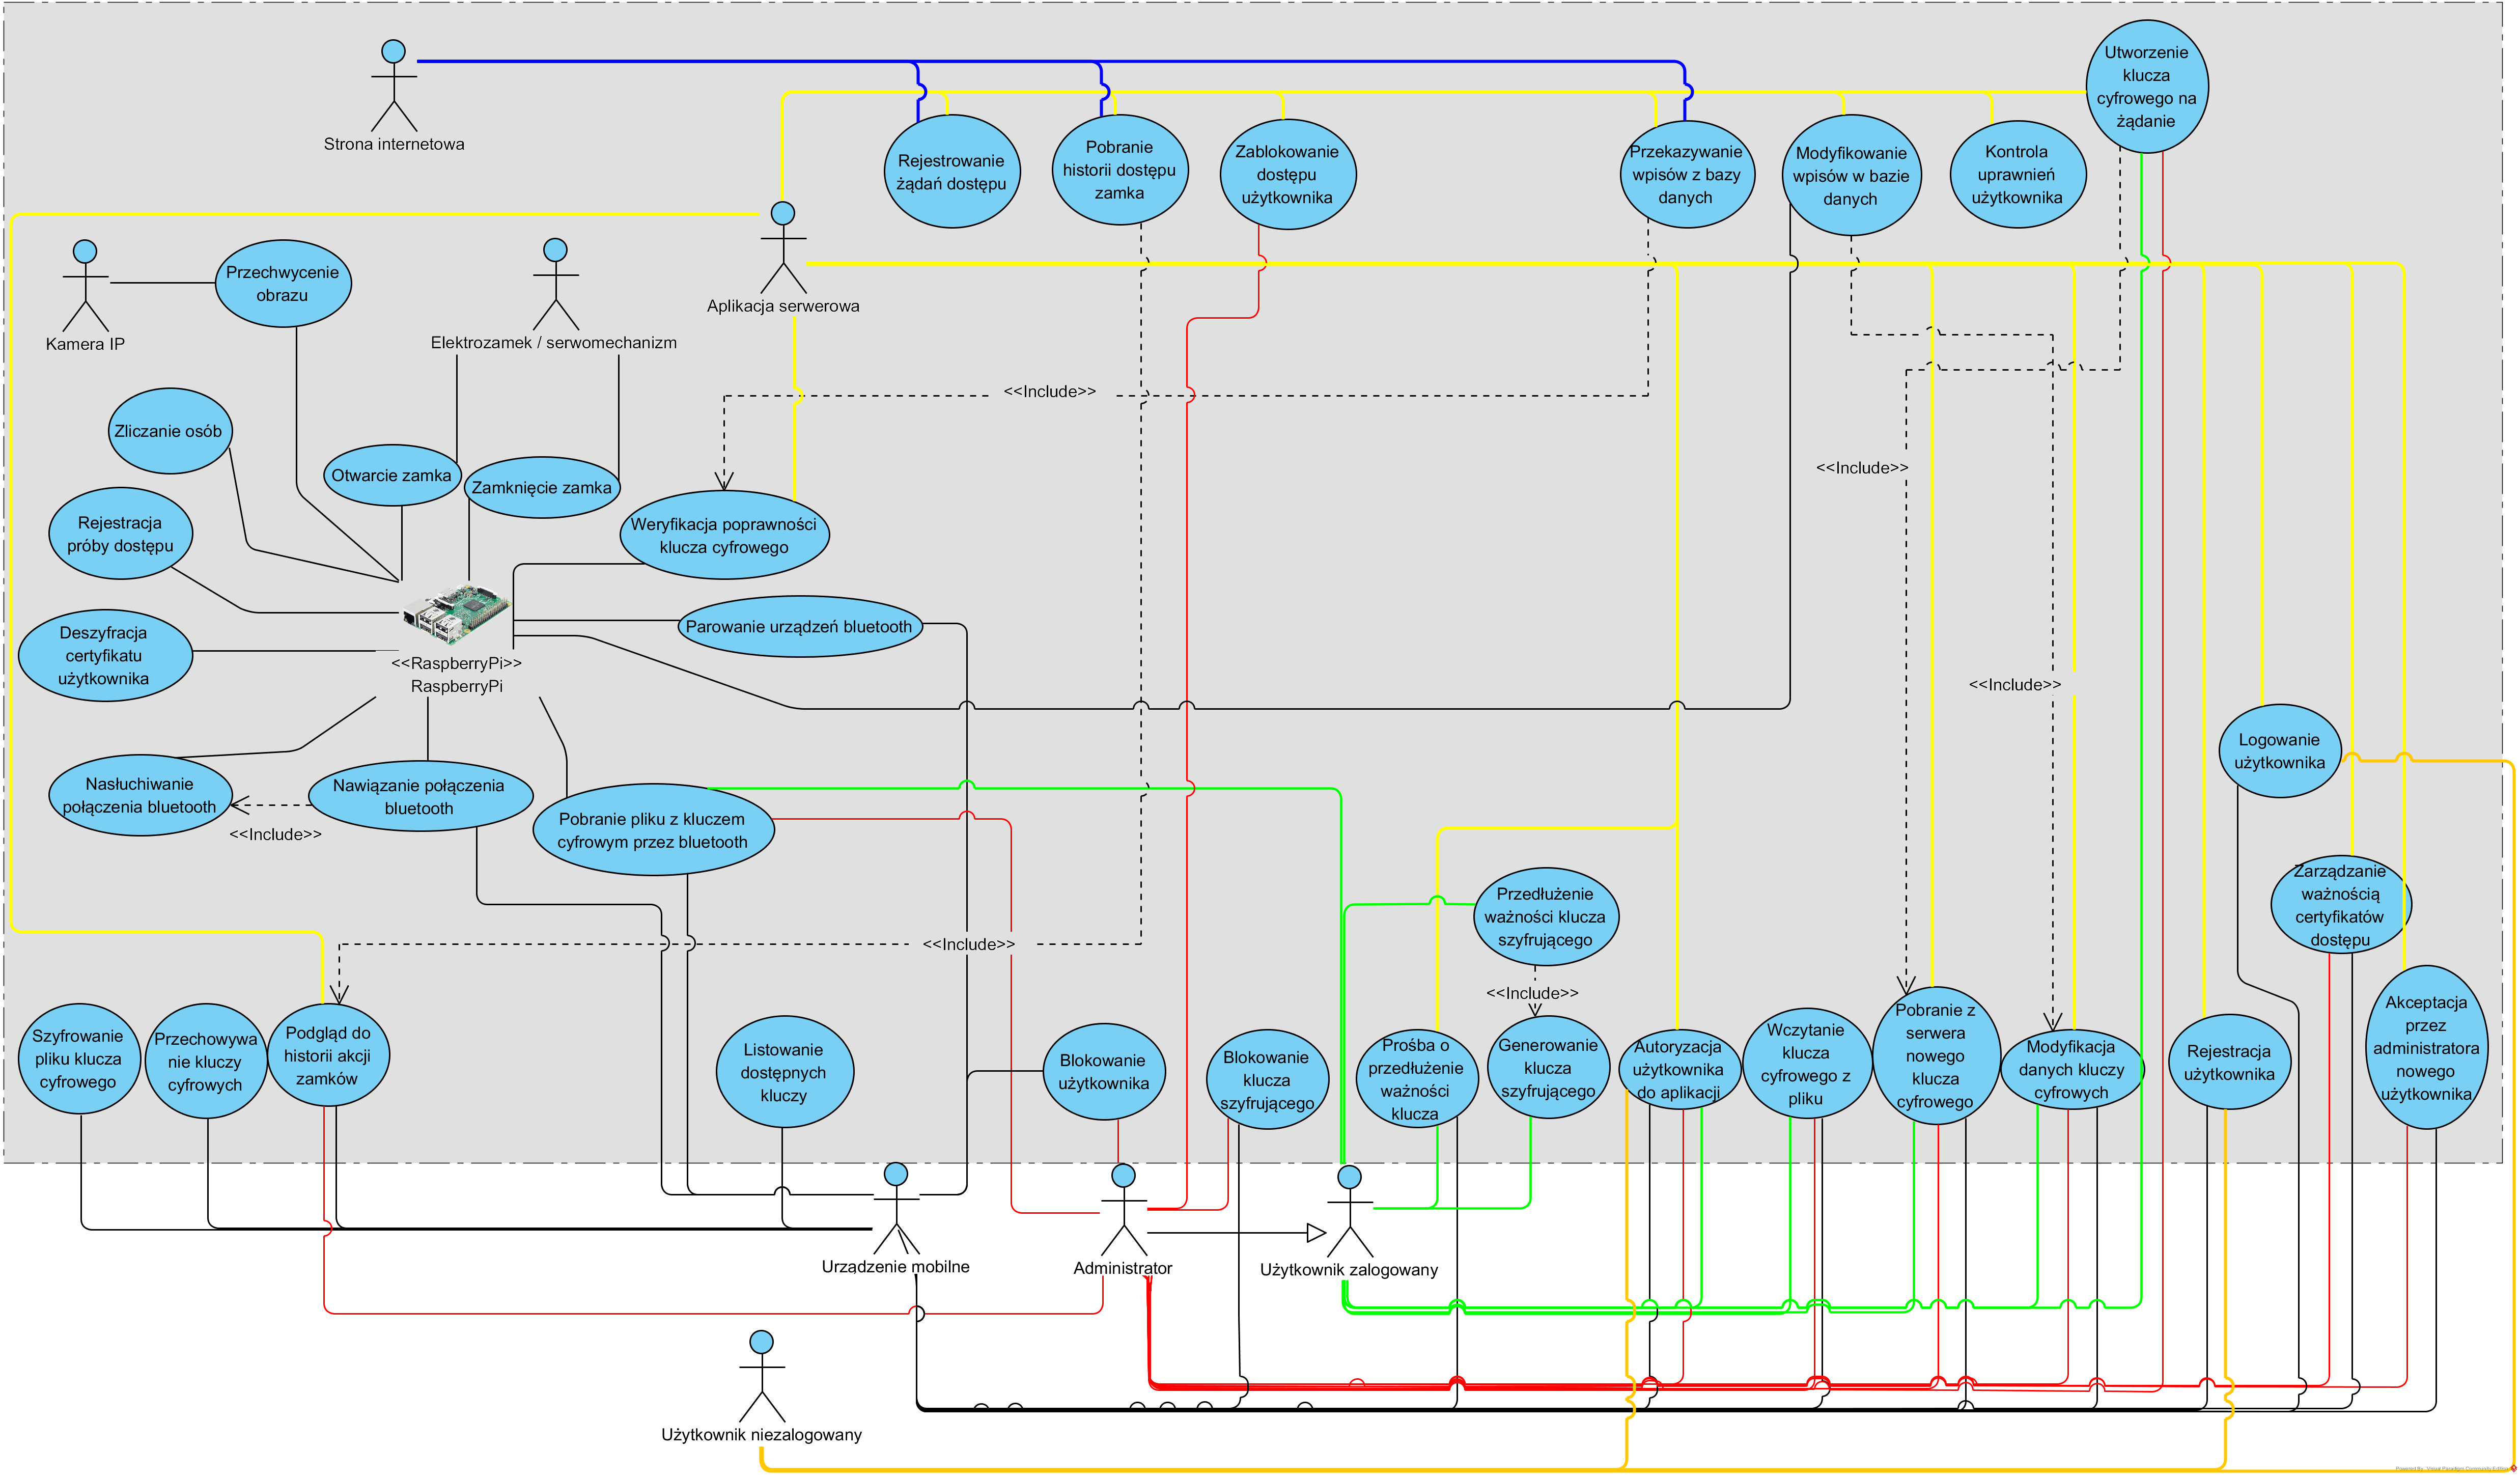
\includegraphics[width=24cm]{Obrazy/Diagram_przypadkow_uzycia.png}
\caption{Diagram przypadków użycia}
\label{diagram:diagram przypadków_użycia}
\end{figure}
\end{landscape}
\newpage
\subsubsection{Projekt bazy danych [Maciej Marciniak]} 
Baza danych będzie składać się z pięciu tabel:
\begin{itemize*}
\item {USERS} --- przechowuje dane użytkowników oraz dane niezbędne przy weryfikacji logowania,
\item {LOCKS} --- zawiera informacje na temat dostępnych w systemie zamków,
\item {ACCESS\_TO\_LOCKS} --- archiwizuje próby użycia certyfikatów,
\item {LOCKS\_KEYS} --- zawiera wszystkie klucze dostępowe użytkowników,
\item {WAIT\_LOCKS\_KEYS} --- przetrzymuje klucze dostępowe oczekujące na zatwierdzenie przez administratora.
\end{itemize*}

Wiersz tabeli USERS zawierać musi:
\begin{itemize*}
\item {ID\_USER} --- unikalny identyfikator (klucz główny) użytkownika składający się z 10 cyfr,
\item {LOGIN} --- unikalna nazwa użytkownika niezbędna podczas logowania, zawierająca nie więcej niż 255 znaków,
\item {PASSWORD} --- hasło zapisane w postaci skrótu, potrzebne do autoryzacji dostępu użytkownikowi,
\item {NAME} - imię użytkownika,
\item {SURNAME} --- nazwisko użytkownika,
\item {TOKEN} --- generowany ciąg pseudolosowy klucz sesji logowania,
\item  {ISACTIVATED} --- pole boolowskie oznaczające, czy dane konto jest zaakceptowane,
\item {IS\_ADMIN} --- pole boolowskie wskazujące czy dany użytkownik jest administratorem czy nie, (aktywowane) przez administratora.
\item {PUBLIC\_KEY} --- klucz publiczny użytkownika potrzebny do podpisu cyfrowego,
\item Serial\_number --- unikalny numer seryjny certyfikatu szyfrującego,
\item Validity\_period --- data, do której ważny jest certyfikat szyfrujący,
\item Version --- numer wersji certyfikatu szyfrującego,
\item Signature\_Algorithm\_Identifier --- identyfikator algorytmu szyfrującego,
\item Hash\_Algorithm --- identyfikator algorytmu funkcji skrótu.
\end{itemize*}

Klucz dostępowy składa się z:
\begin{itemize*}
\item {ID\_KEY} --- unikalny identyfikator (klucz główny) klucza dostępowego składający się z 10 cyfr,
\item {ID\_LOCK} --- klucz obcy do tabeli przechowującej dostępne zamki,
\item {ID\_USER} --- klucz obcy do tabeli przechowującej dane użytkownika, jest to pole służące do określenia kto utworzył klucz dostępu,
\item {LOCK\_KEY} --- unikalna wartość certyfikatu dostępu,
\item {FROM\_DATE} --- data, od której obowiązuje klucz,
\item {TO\_DATE} --- data, do której obowiązuje klucz,
\item {ISACTUAL} --- data wygaśnięcia klucza, jeśli równa TO, oznacza to że klucz utracił ważność z powodu czasu, jeśli różna oznacza, to że zablokowano z innego powodu ważność,
\item {MONDAY} --- słowne określenie, w których godzinach zostanie przyznany dostęp w poniedziałki,
\item {TUESDAY} --- słowne określenie, w których godzinach zostanie przyznany dostęp we wtorki,
\item {WEDNESDAY} --- słowne określenie, w których godzinach zostanie przyznany dostęp w środy,
\item {THURSDAY} --- słowne określenie, w których godzinach zostanie przyznany dostęp w czwartki,
\item {FRIDAY} --- słowne określenie, w których godzinach zostanie przyznany dostęp w piątki,
\item {SATURDAY} --- słowne określenie, w których godzinach zostanie przyznany dostęp w soboty,
\item {SUNDAY} --- słowne określenie, w których godzinach zostanie przyznany dostęp w niedziele,
\item {IS\_PERNAMENT} --- zmienna boolowska oznaczająca czy dostęp jest zawsze,
\item {NAME} - imię osoby, której dotyczy certyfikat,
\item {SURNAME} --- nazwisko osoby, której dotyczy certyfikat.
\end{itemize*}

\newpage
Zamek opisywany jest poprzez kolumny:
\begin{itemize*}
\item {ID\_LOCK} --- unikalny identyfikator (klucz główny) zamka składający się z 10 cyfr,
\item {NAME} --- unikalna nazwa zamka,
\item {MAC\_ADDRESS} --- adres fizyczny urządzenia sterującego zamkiem,
\item {LOCALIZATION} --- nieobowiązkowe pole opisujące fizyczne położenie zamka,
\item {People\_inside} --- wartość licznika osób znajdujących się wewnątrz pomieszczenia.
\end{itemize*}

W tabeli archiwizującej akcje na zamku znajdują się takie dane jak:
\begin{itemize*}
\item {ID} --- unikalny identyfikator (klucz główny) akcji wykonanej na certyfikacie składający się z 10 cyfr,
\item {ID\_KEY} --- klucz obcy do tabeli przechowującej klucze dostępowe, dzięki tej informacji możemy uzyskać dane o zamku, który został otwierany jak również do kogo należał klucz,
\item {DATE} --- dokładna data z godziną użycia klucza dostępowego,
\item {ACCESS} --- binarna flaga informująca czy dostęp został przyznany czy odmówiony.
\end{itemize*}

Tabela WAIT\_LOCKS\_KEYS składa się z:
\begin{itemize*}
\item {ID\_KEY} --- unikalny identyfikator (klucz główny) oczekującego certyfikatu,
\item{ID\_LOCK} --- klucz obcy do tabeli LOCKS, oznacza zamek, do którego jest zgłaszana prośba dostępu,
\item {ID\_USER} --- klucz obcy do tabeli USERS, oznacza użytkownika, który zgłasza prośbę o dostęp do zamka.
\end{itemize*}

Diagramy bazy danych odpowiednio encji i relacji przedstawione zostały na Rys \ref{diagram:diagram encji} i Rys. \ref{diagram:diagram relacji}\cite{BD}.  

\begin{figure}[!h]
\centering
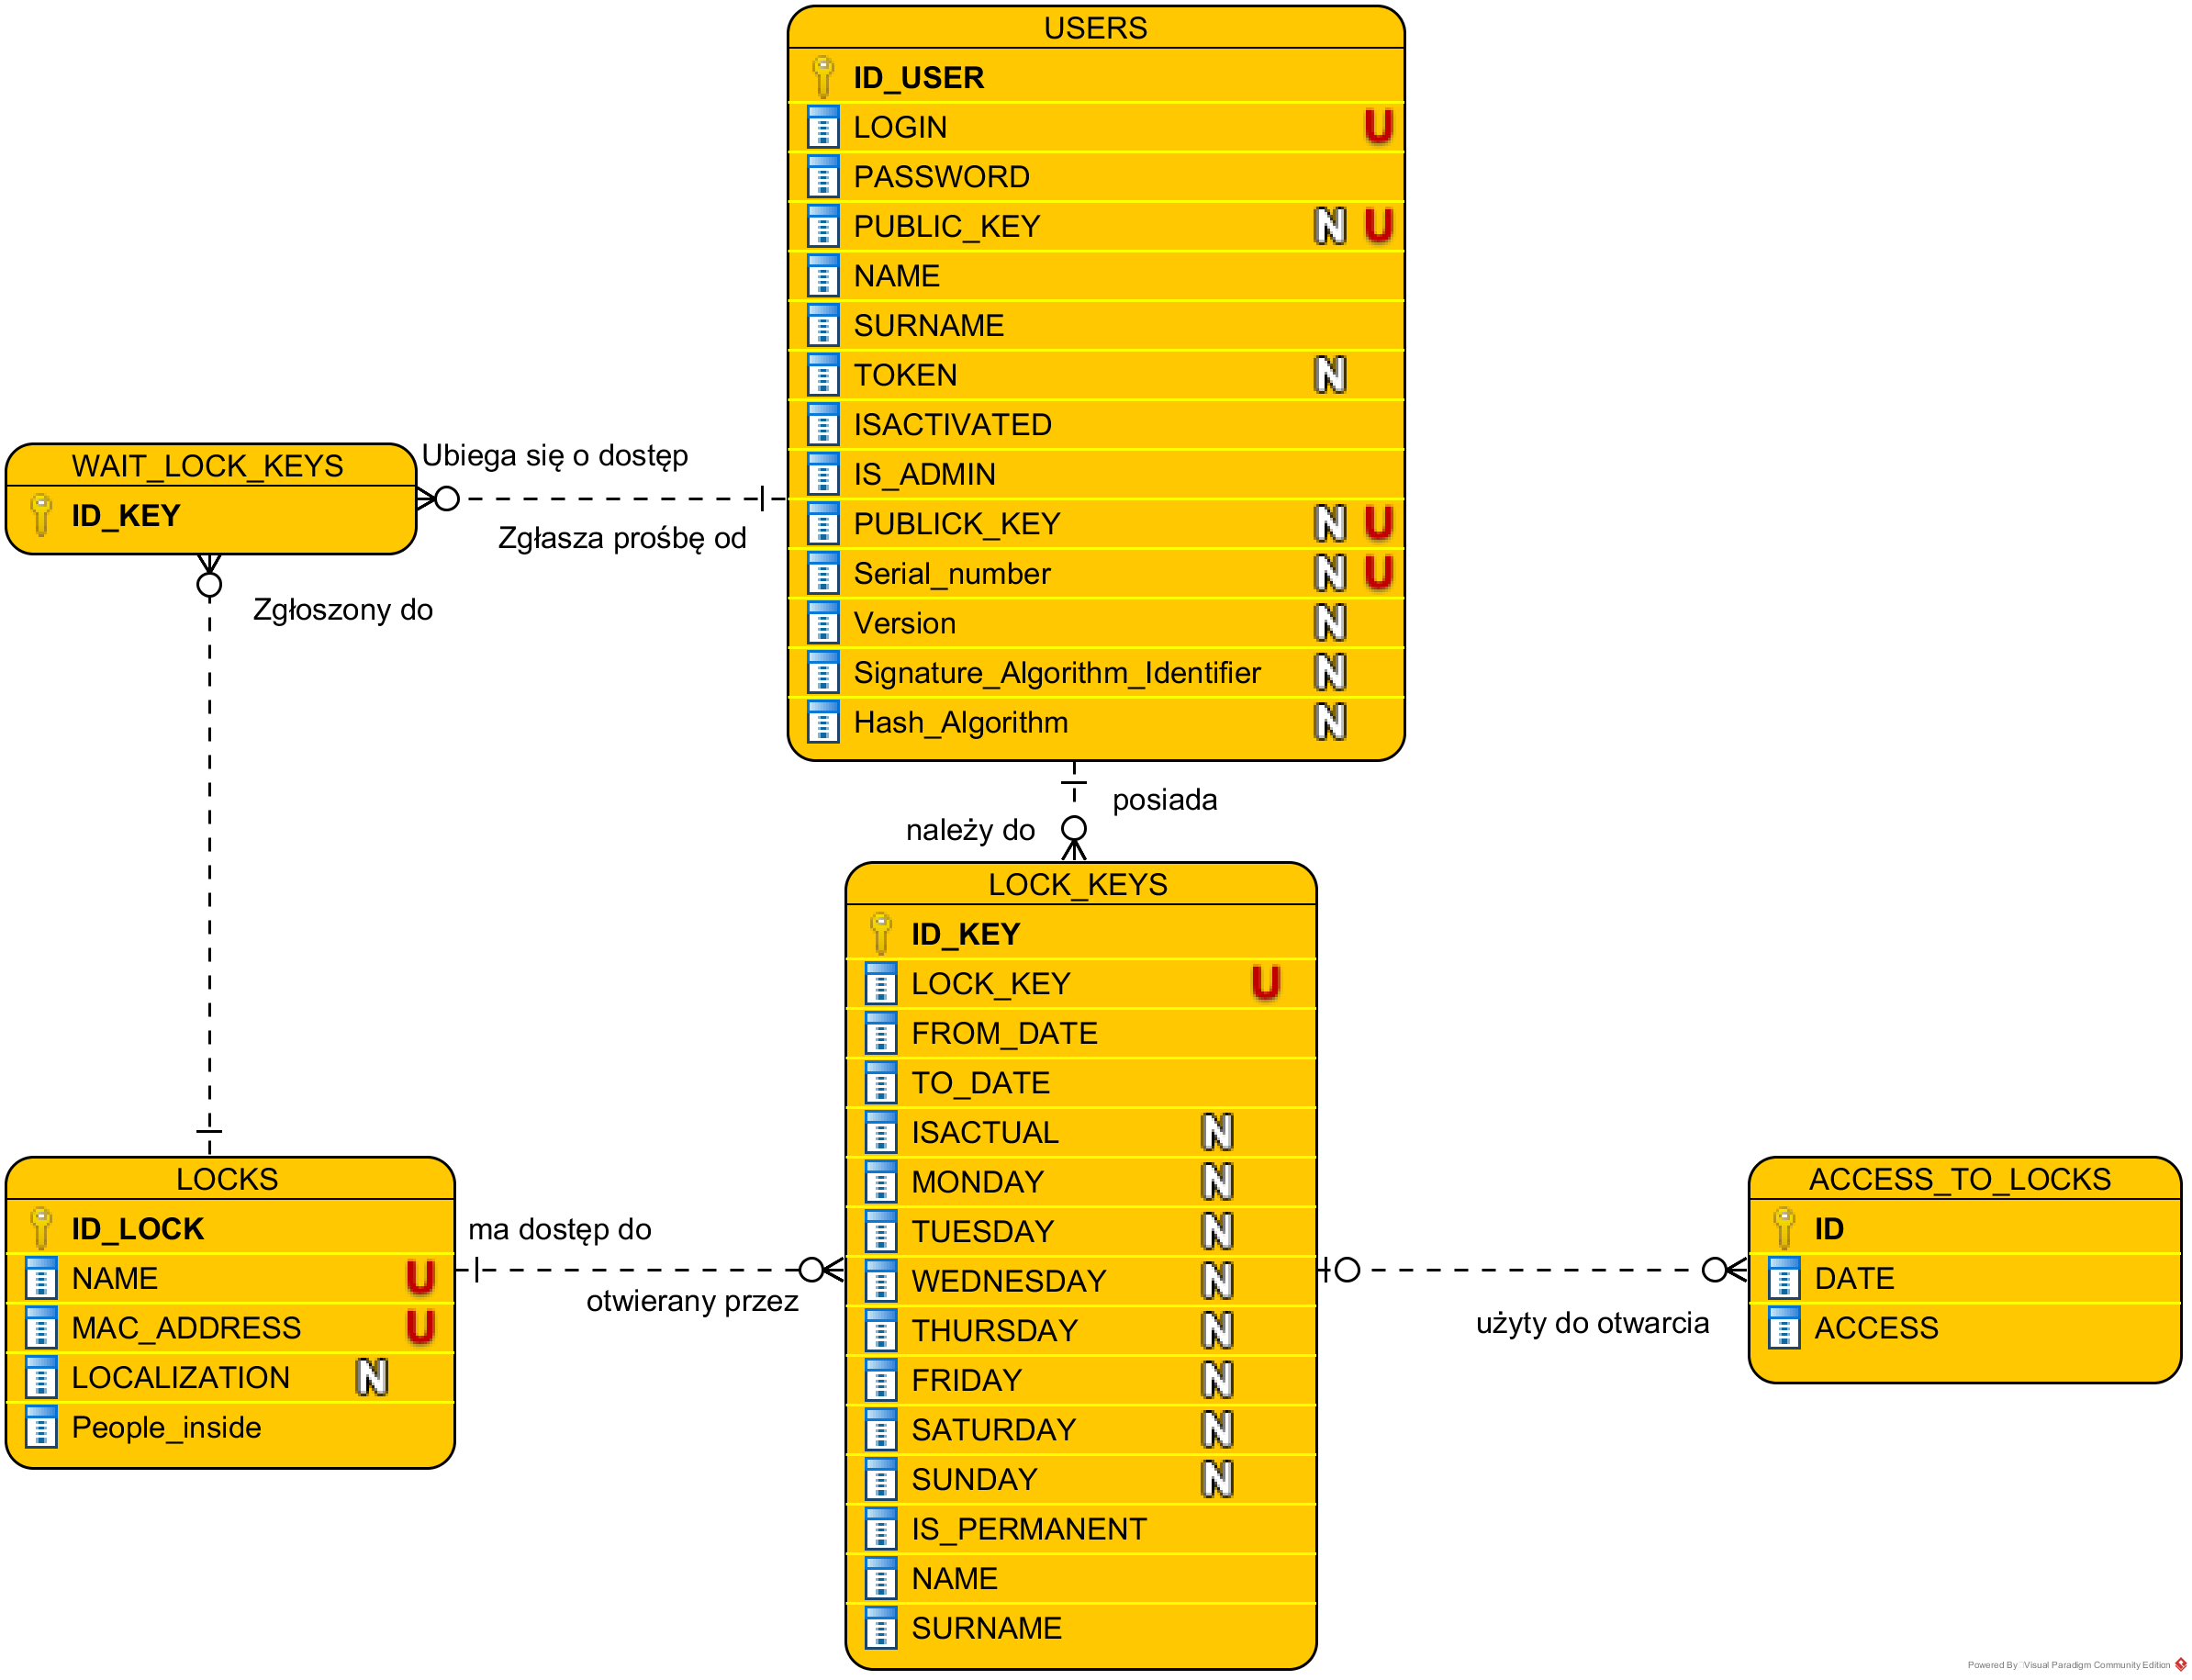
\includegraphics[width=13cm]{Obrazy/Diagram_encji.png}
\caption{Diagram encji bazy danych}
\label{diagram:diagram encji}
\end{figure}
\newpage
\begin{figure}[!h]
\centering
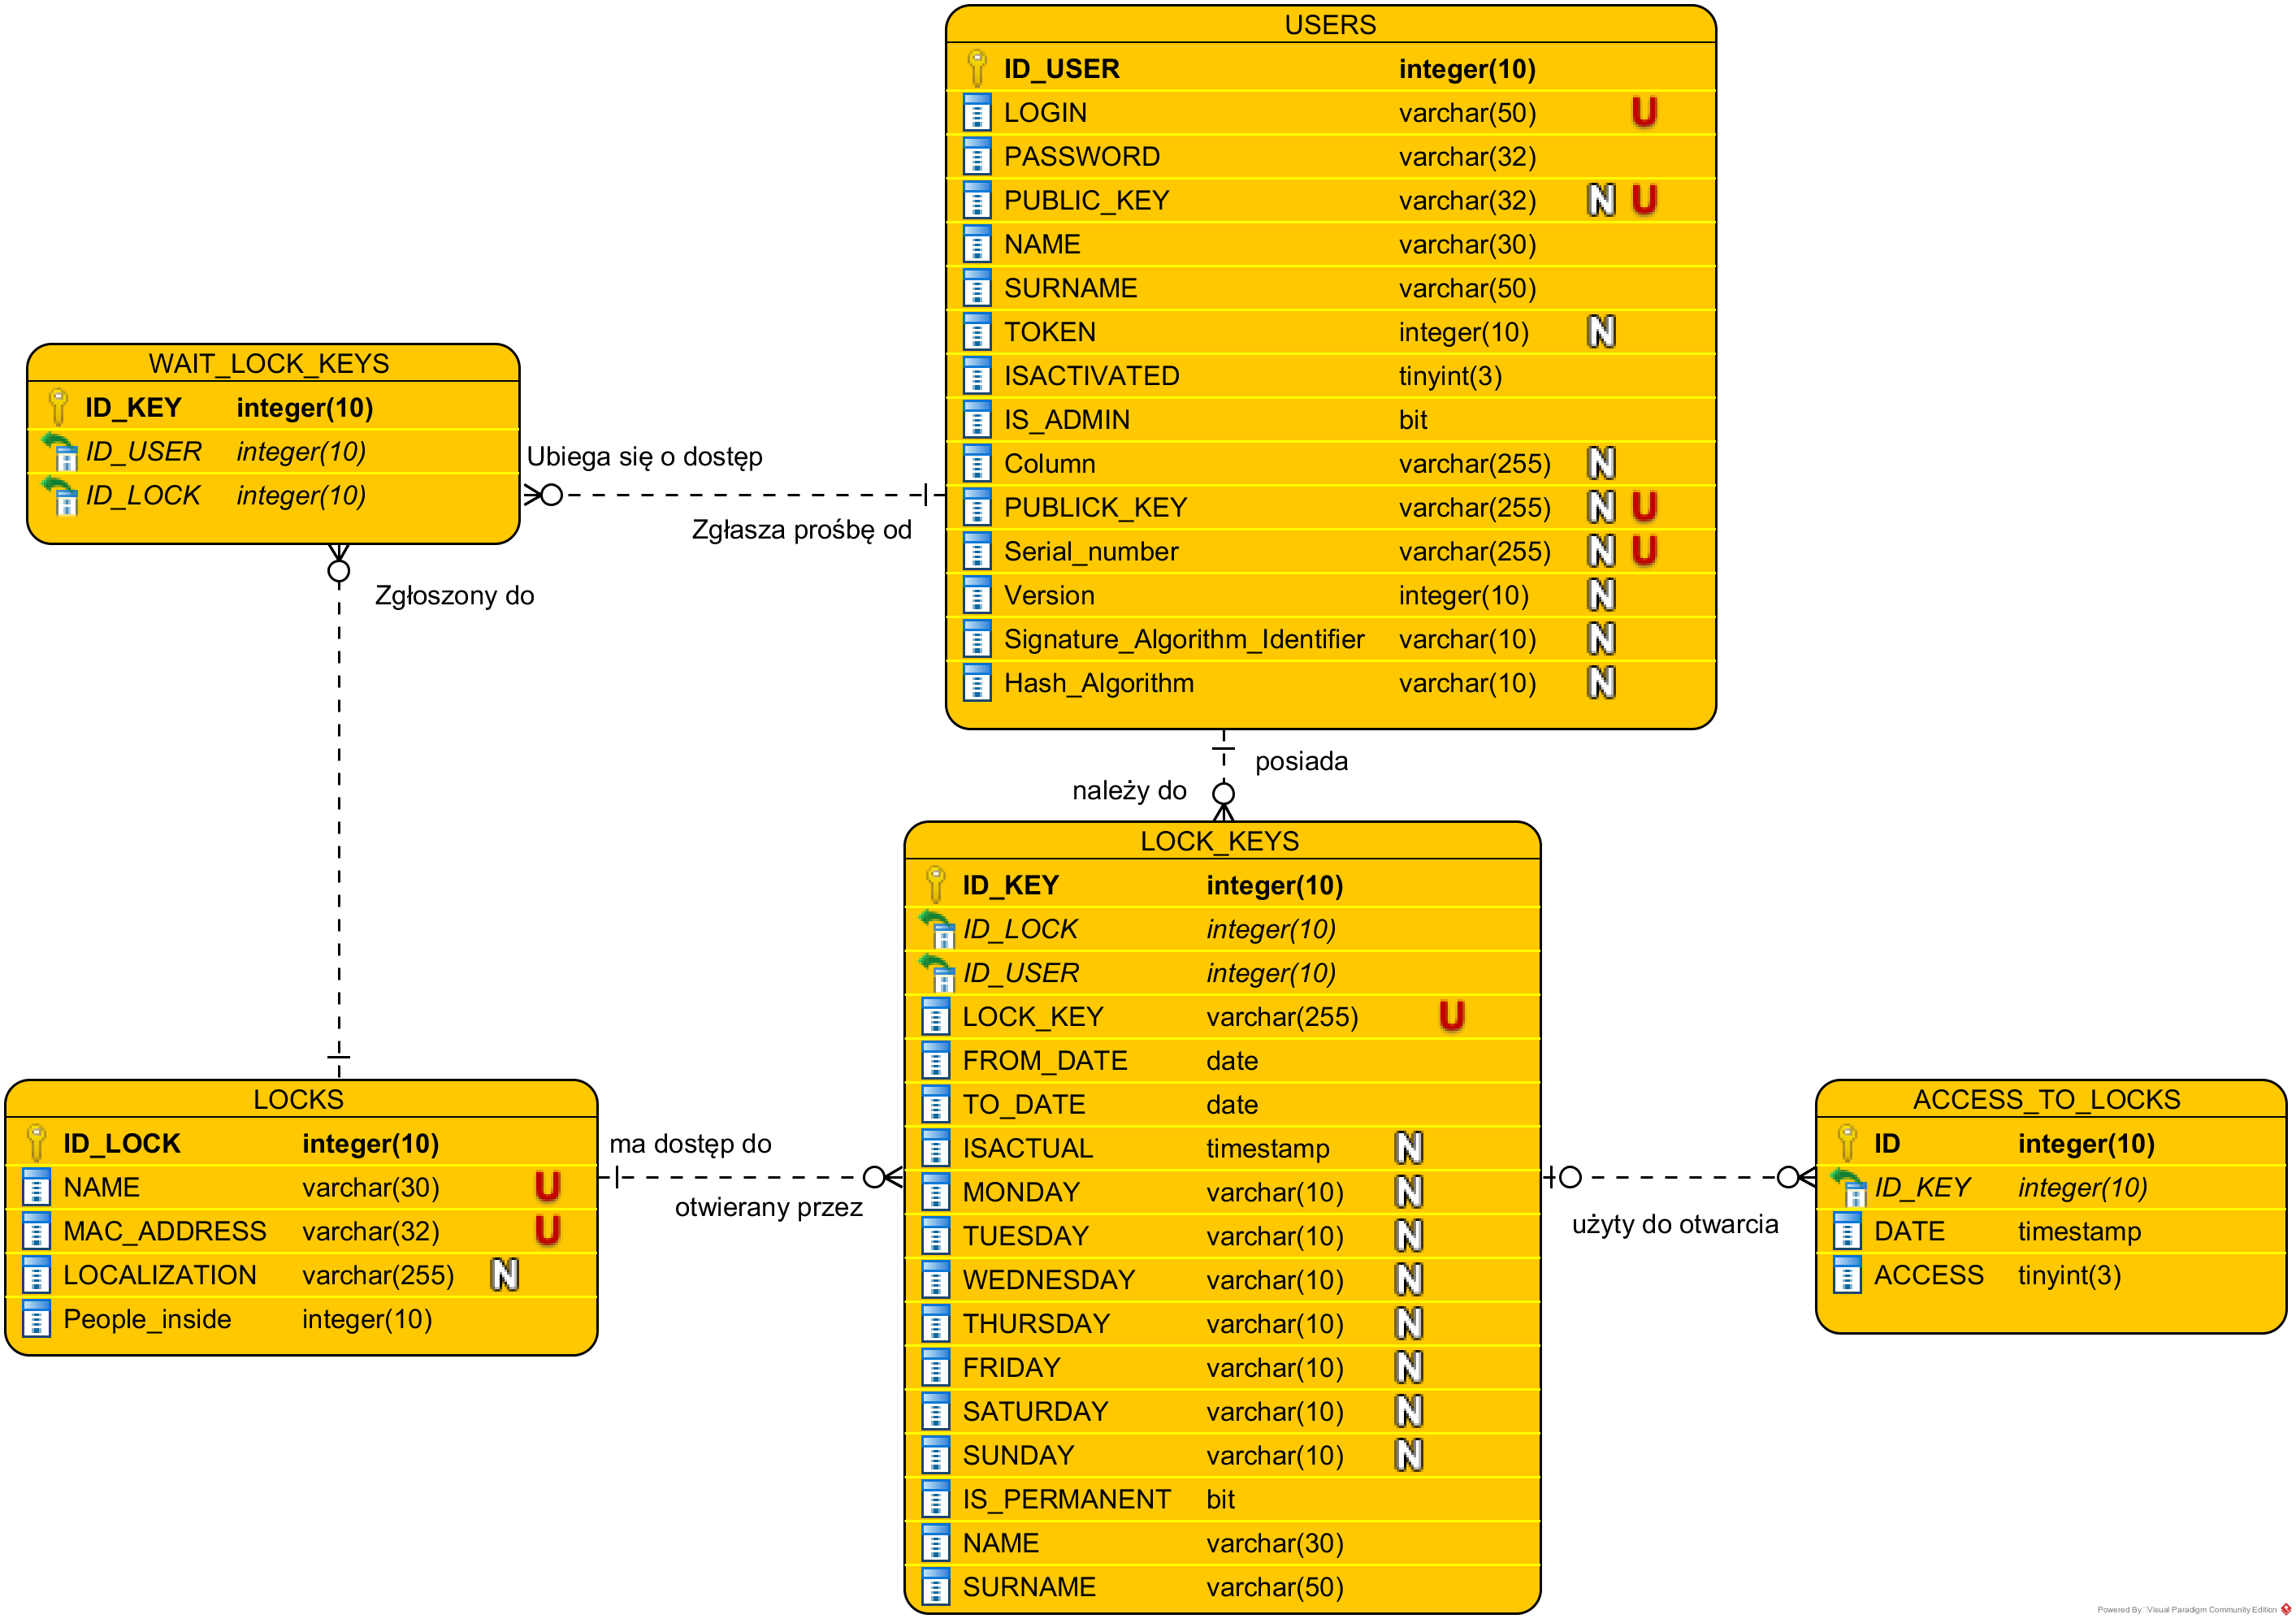
\includegraphics[width=13cm]{Obrazy/Diagram_relacji.png}
\caption{Diagram relacji bazy danych}
\label{diagram:diagram relacji}
\end{figure}
\newpage

\subsubsection{Diagramy klas}\label{sec:diagramy klas}
Rozdział \ref{sec:diagramy klas} przedstawia struktury danych potrzebne do zrealizowania projektu. Jeżeli diagramy posiadają ze sobą więzi, np. jedna klasa używa obiektów drugiej, wtedy zostają połączone relacjami różnego typu. Połączenia przedstawione jako przerywane linie oznaczają relację \textit{use}, to znaczy, są sporadycznie używane pomiędzy sobą, lecz nie są w stałym użyciu. Drugą relacją znajdującą się na schematach jest linia ciągła zakończona rombem, oznaczająca relację ścisłą (klasy mają pomiędzy sobą wspólne obiekty i są używane w częsty sposób). Najsilniejszym z przedstawianych związków jest relacja dziedziczenia, przedstawiana jako linia z zakończonym trójkątnym grotem. Dziedziczenie oznacza przejęcie obiektów klasy przez inną strukturę.
\paragraph*{Aplikacja mobilna [Damian Filipowicz]}
Aplikacja mobilna składa się z szeregu klas napisanych w 2 językach: Kotlin oraz Java. Ponadto klasy te~zostały podzielone na 5 kategorii (Rys. \ref{Schemat ogólny diagramu klas dla Aplikacji mobilnej}) takich jak:

\begin{itemize*}
\item API 
(Rys. \ref{Diagram klas dla paczki api}) 
---  które przechowuje klasy odpowiedzialne za funkcje wykorzystywane w wielu miejscach systemu. W paczce znajdują się klasy odpowiedzialne między innymi za odczyt oraz zapis do pliku, komunikacje HTTPS, czy wykorzystywanie SharedPreferences w aplikacji ,
\item Navigation 
(Rys. \ref{Diagram klas dla paczki navigations}) 
--- są to klasy odpowiedzialne za generowanie nawigacji w aplikacji mobilnej. Paczka znajdują się 4 klasy,
\item Adapters
(Rys. \ref{Diagram klas dla paczki adapters}) 
--- w którym są przechowywane klasy adapter wykorzystywane w systemie do wyświetlania danych.
\end{itemize*}

\begin{figure}[ht!]
\centering
\vspace{-0.6cm}
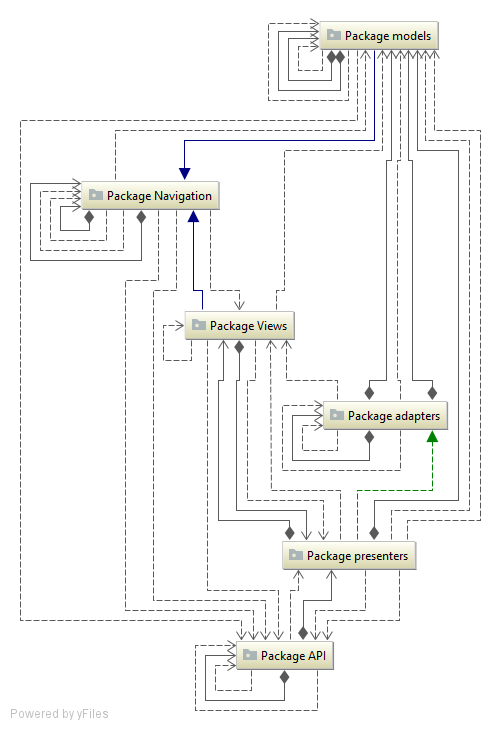
\includegraphics[width=9cm]{Obrazy/AM_DK_ALL}
\caption{Schemat ogólny diagramu klas dla Aplikacji Mobilnej}
\label{Schemat ogólny diagramu klas dla Aplikacji mobilnej}
\end{figure}
\newpage
\begin{figure}[ht!]
\centering
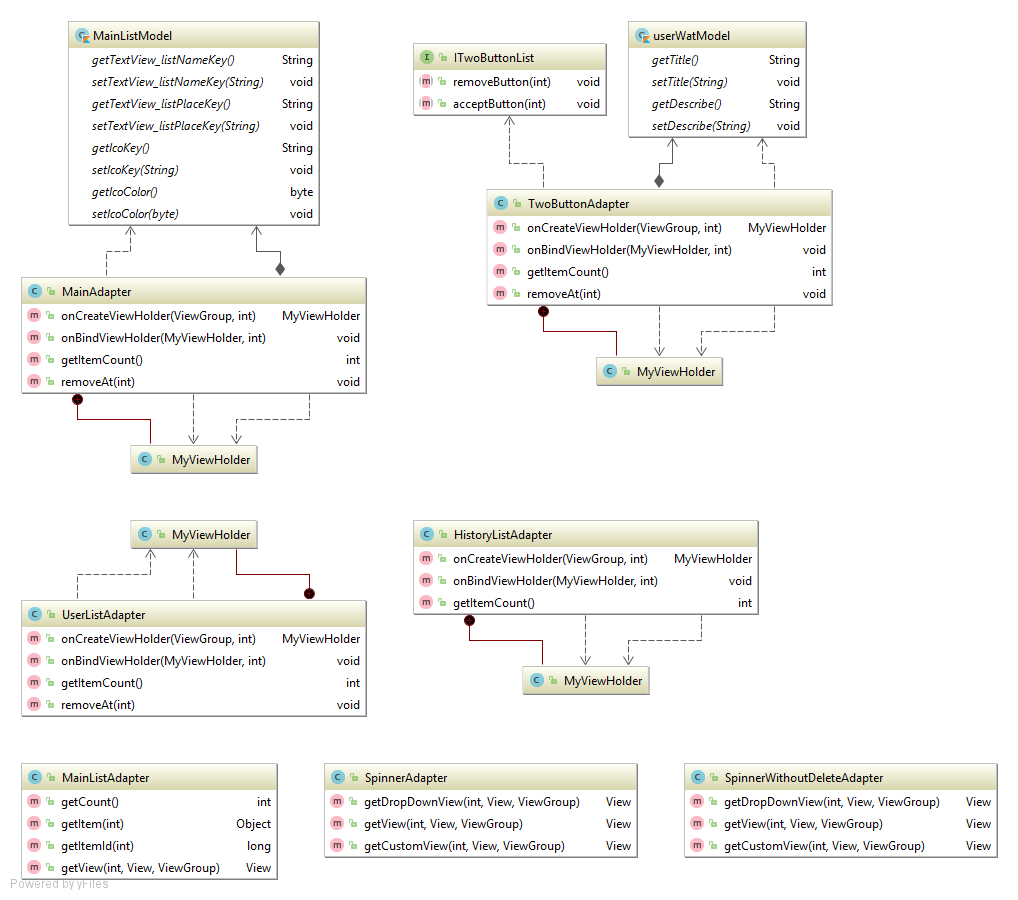
\includegraphics[width=16cm]{Obrazy/AM_DK_adapter}
\caption{Diagram klas dla paczki adapters}
\label{Diagram klas dla paczki adapters}
\end{figure}
\newpage
\begin{figure}[ht!]
\centering
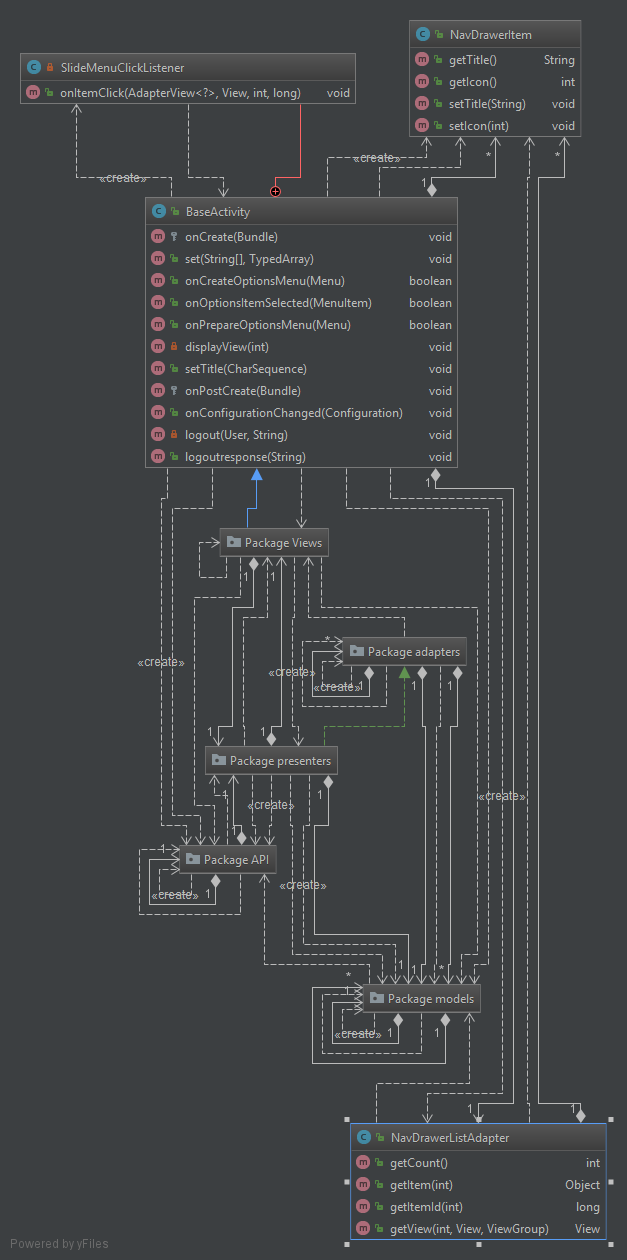
\includegraphics[width=16cm]{Obrazy/AM_DK_navigation}
\caption{Diagram klas dla paczki navigations}
\label{Diagram klas dla paczki navigations}
\end{figure}

Oprócz tych wymienionych wyżej są dodatkowo 3 kategorie implementujące wzorzec architektoniczny Model-View-Presenter i są to odpowiednio:
\begin{itemize*}
\item Model (Rys. \ref{Diagram klas dla paczki models}) 
--- przechowujący klasy modele odpowiedzialne za przechowywanie danych. Każda z klas która jest powiązana z odpowiednim widokiem   w nazwie na początku ma nazwę widoku a na końcu~ma słowo Model,   
\item View 
(Rys. \ref{Diagram klas dla paczki views}) 
--- przechorowujący klasy widoków odpowiedzialne za generowanie widoków w aplikacji. Każda z klas która jest powiązana z odpowiednim widokiem   w nazwie na początku ma nazwę widoku, a~na~końcu ma słowo Activity, 
\item Presenter
(rysunek \ref{Diagram klas dla paczki presenters}) 
--- przechowujący klasy presenter odpowiedzialne za interakcje pomiędzy modelami oraz widokami. Każda z klas, która jest powiązana z odpowiednim widokiem w nazwie na początku ma nazwę widoku, a na końcu ma słowo Presenter\cite{And}.
\end{itemize*}
\newpage
\begin{figure}[ht!]
\centering
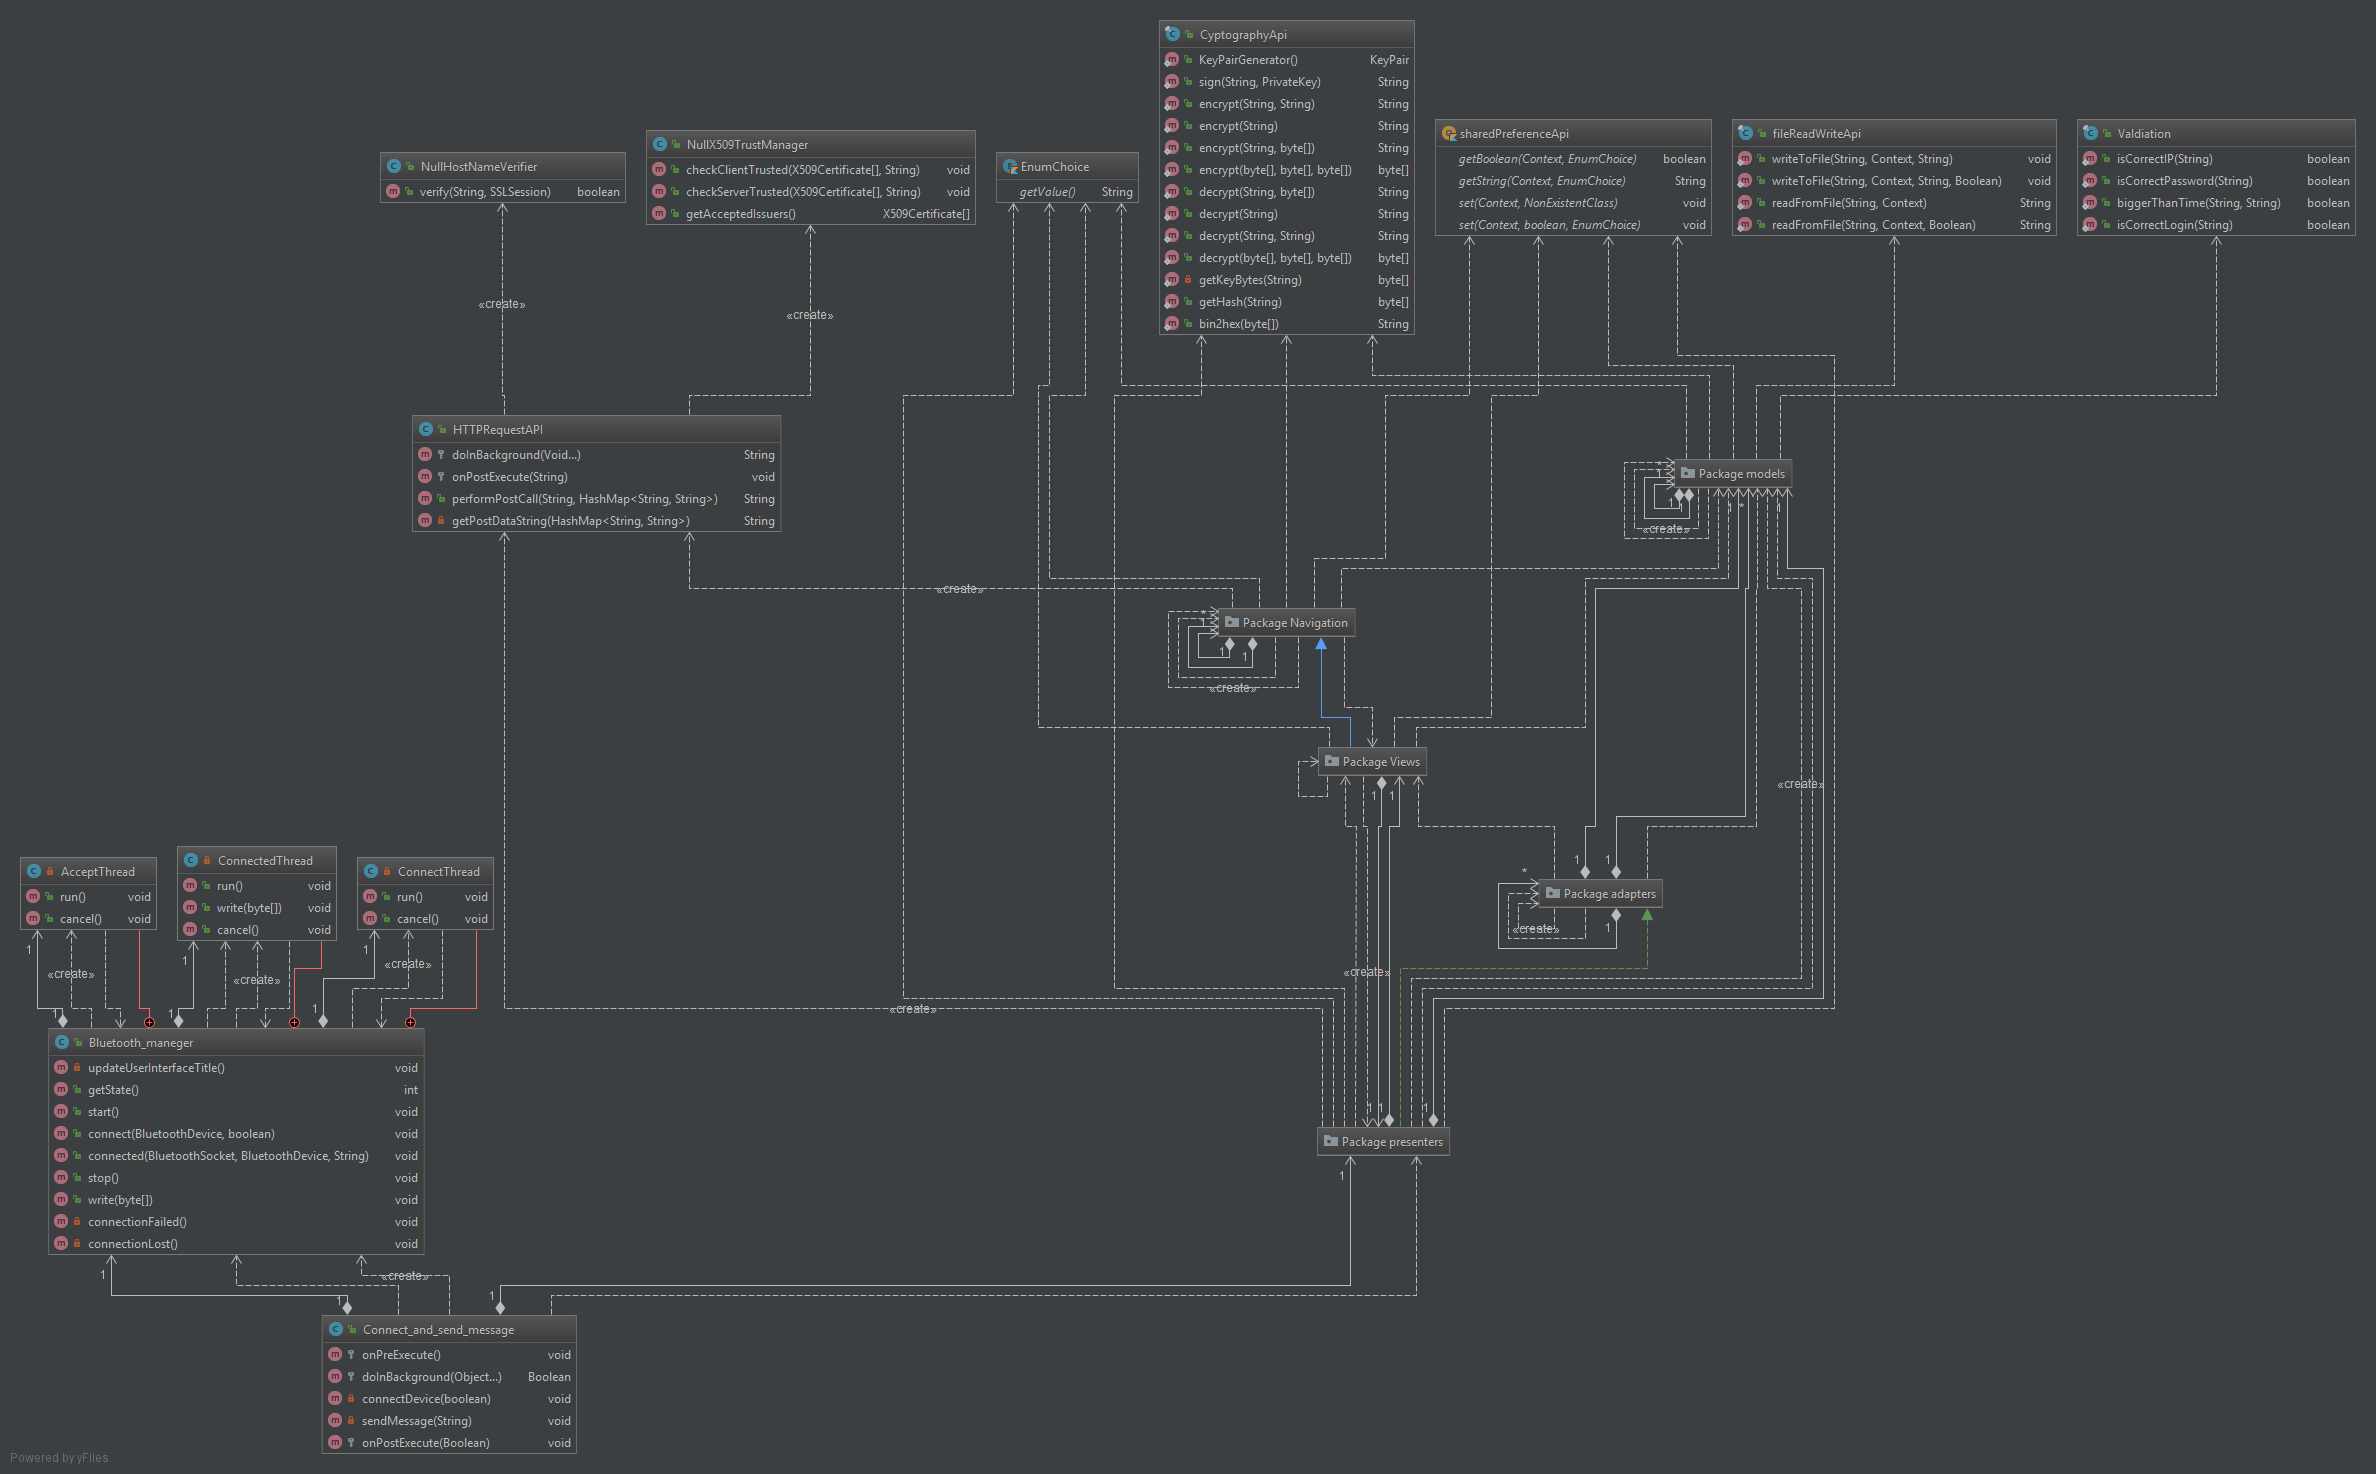
\includegraphics[width=15cm]{Obrazy/AM_DK_api}
\caption{Diagram klas dla paczki api}
\label{Diagram klas dla paczki api}
\end{figure}
\newpage

\newpage
\begin{figure}[ht!]
\centering
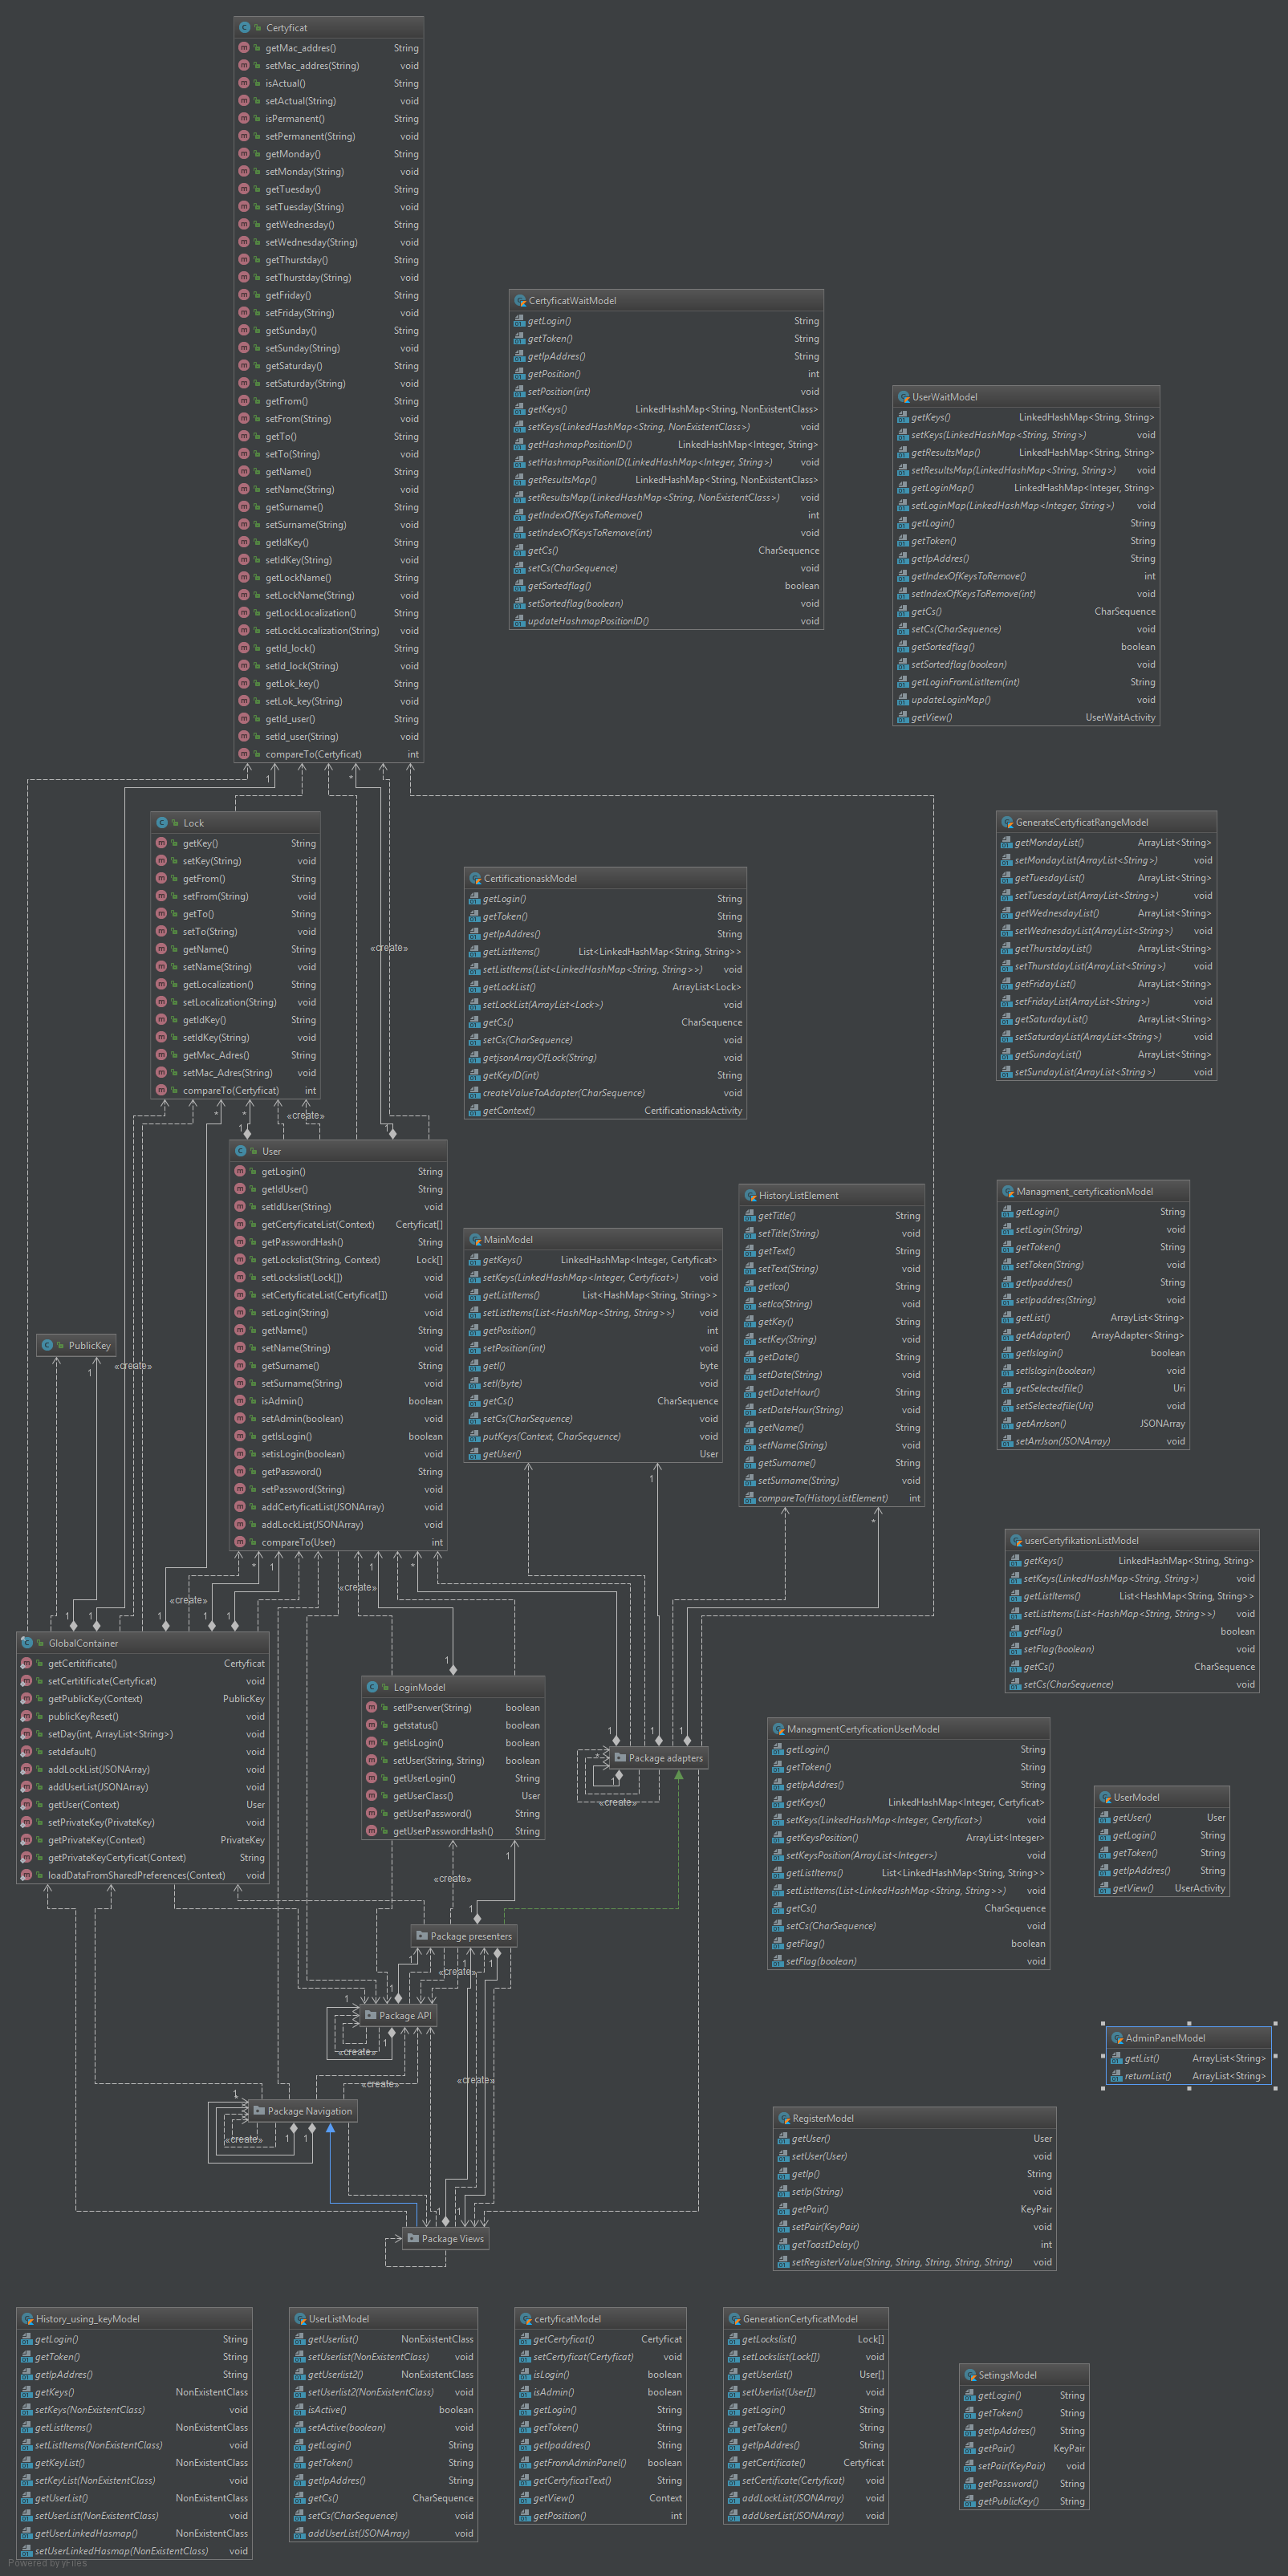
\includegraphics[width=16cm]{Obrazy/AM_DK_model}
\caption{Diagram klas dla paczki models}
\label{Diagram klas dla paczki models}
\end{figure}

\newpage
\begin{figure}[ht!]
\centering
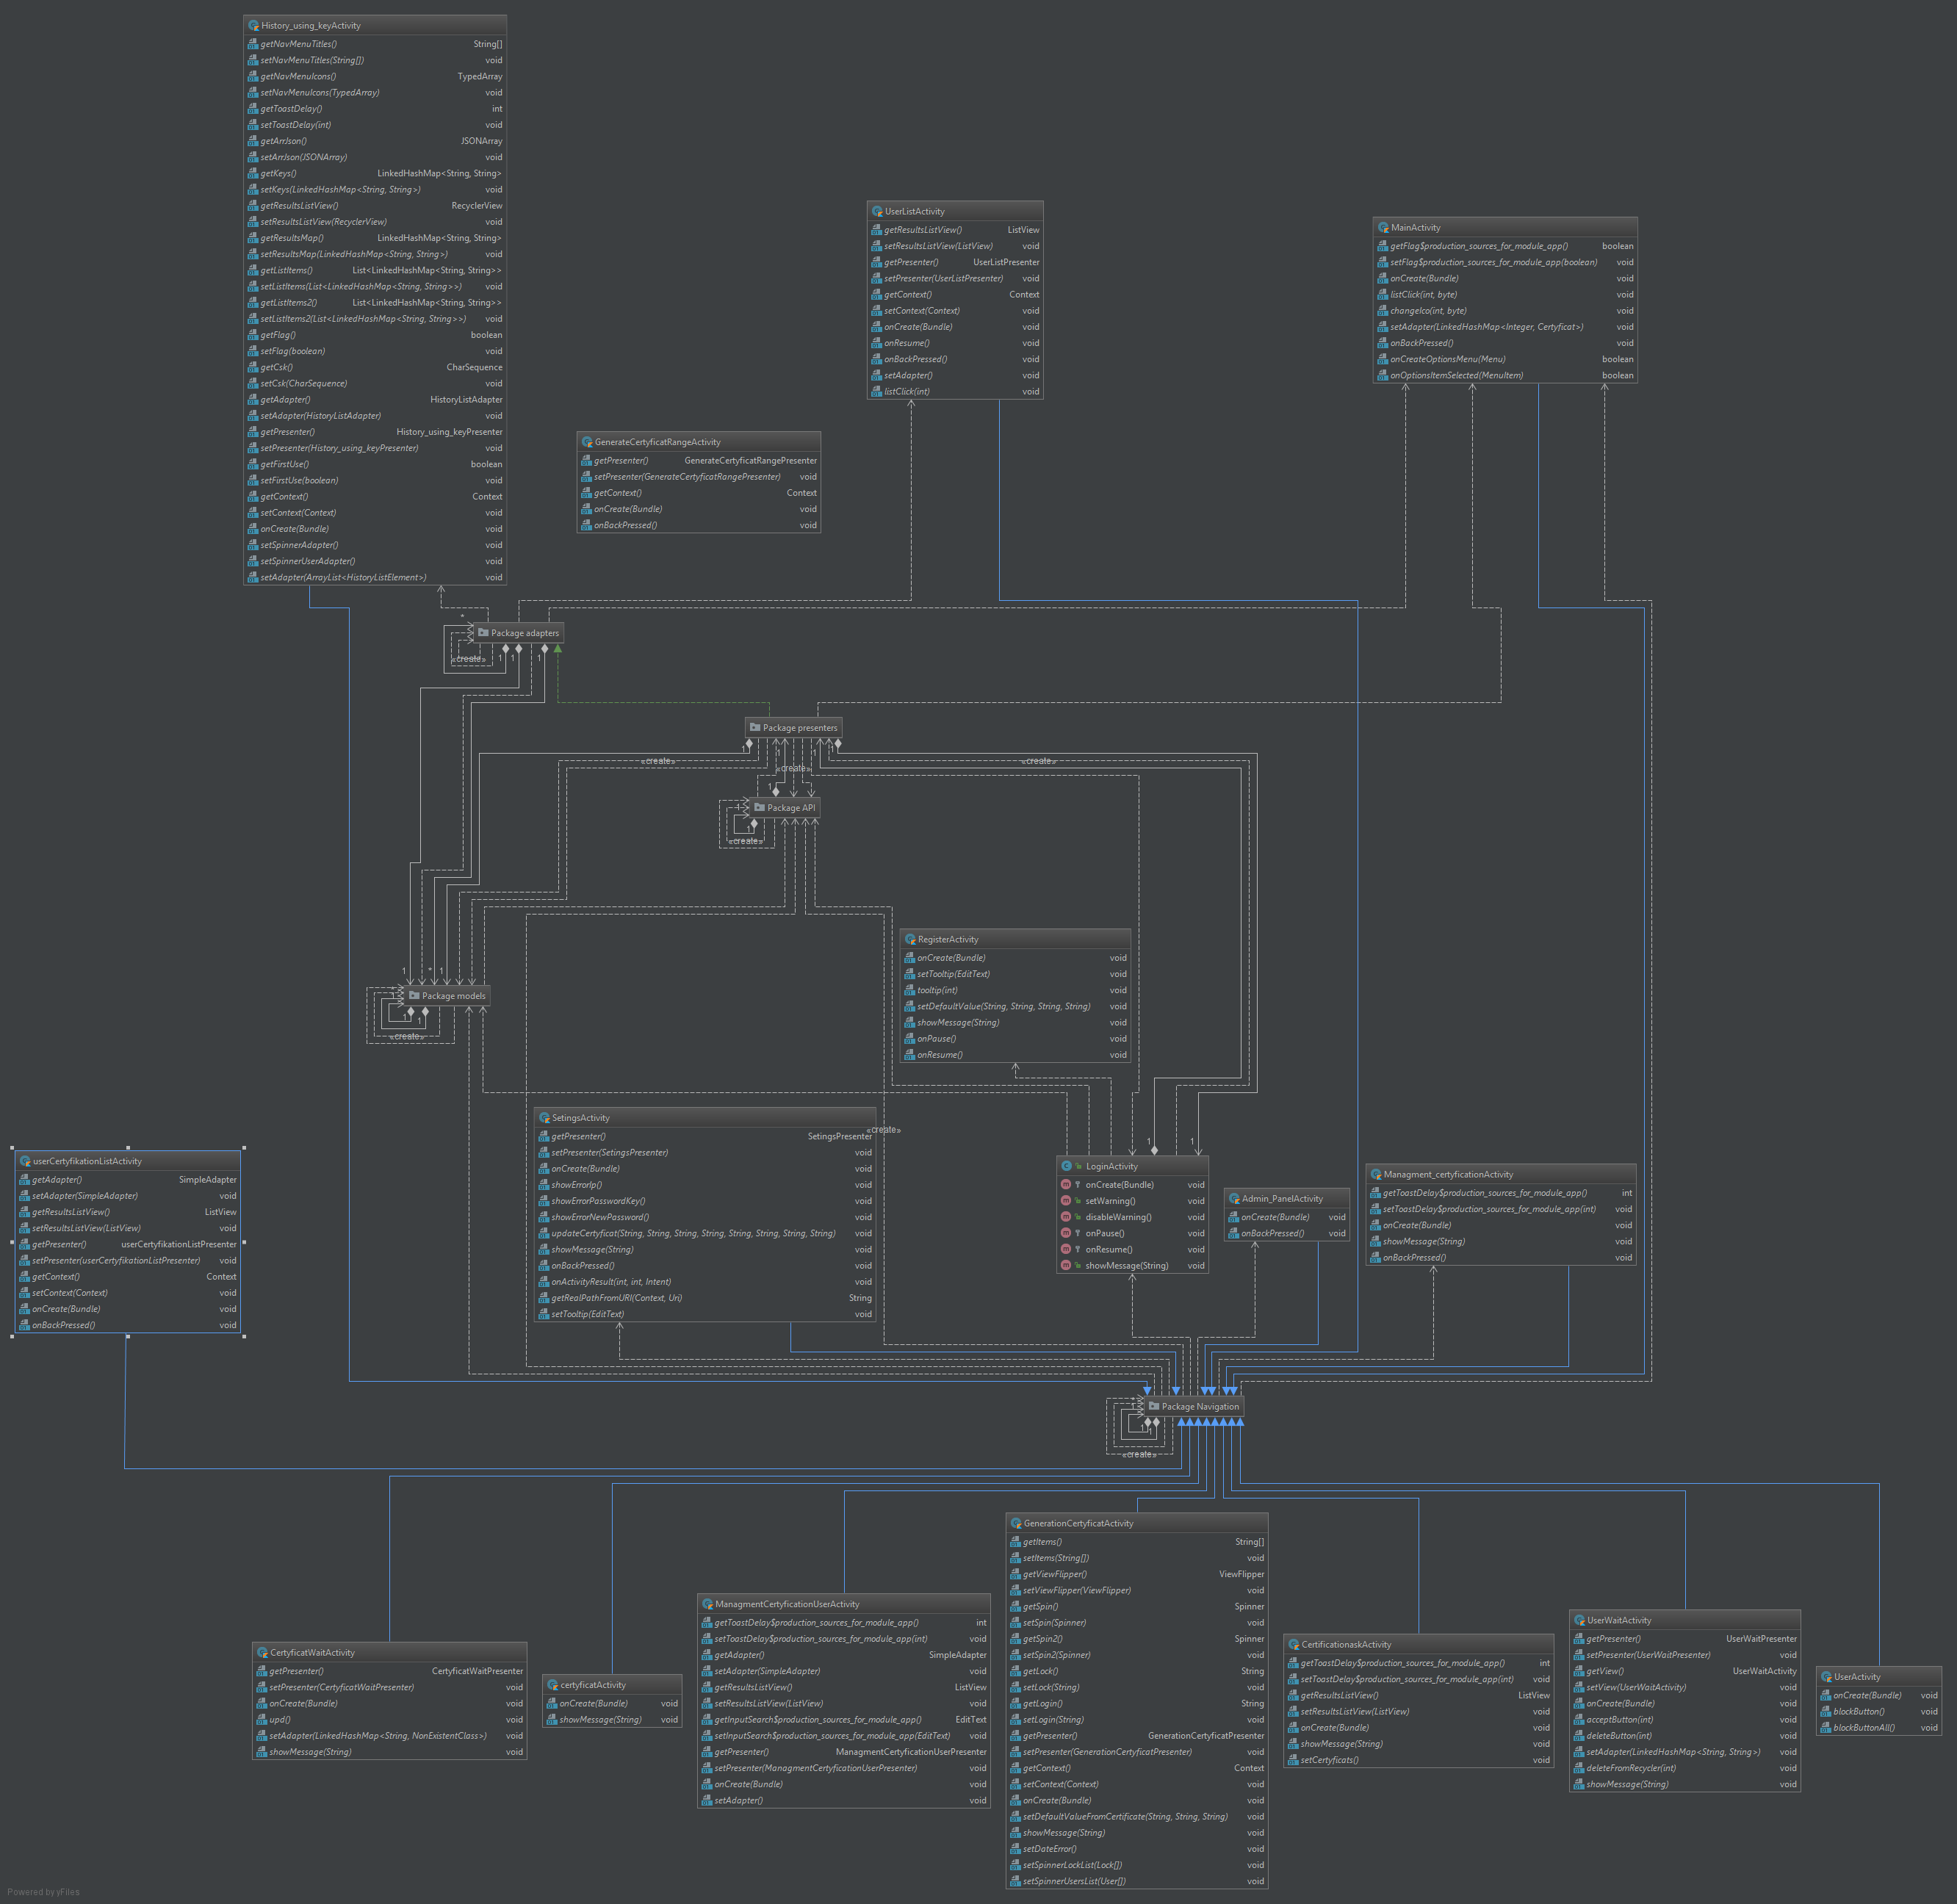
\includegraphics[width=16cm]{Obrazy/AM_DK_view}
\caption{Diagram klas dla paczki views}
\label{Diagram klas dla paczki views}
\end{figure}
\newpage

\begin{figure}[ht!]
\centering
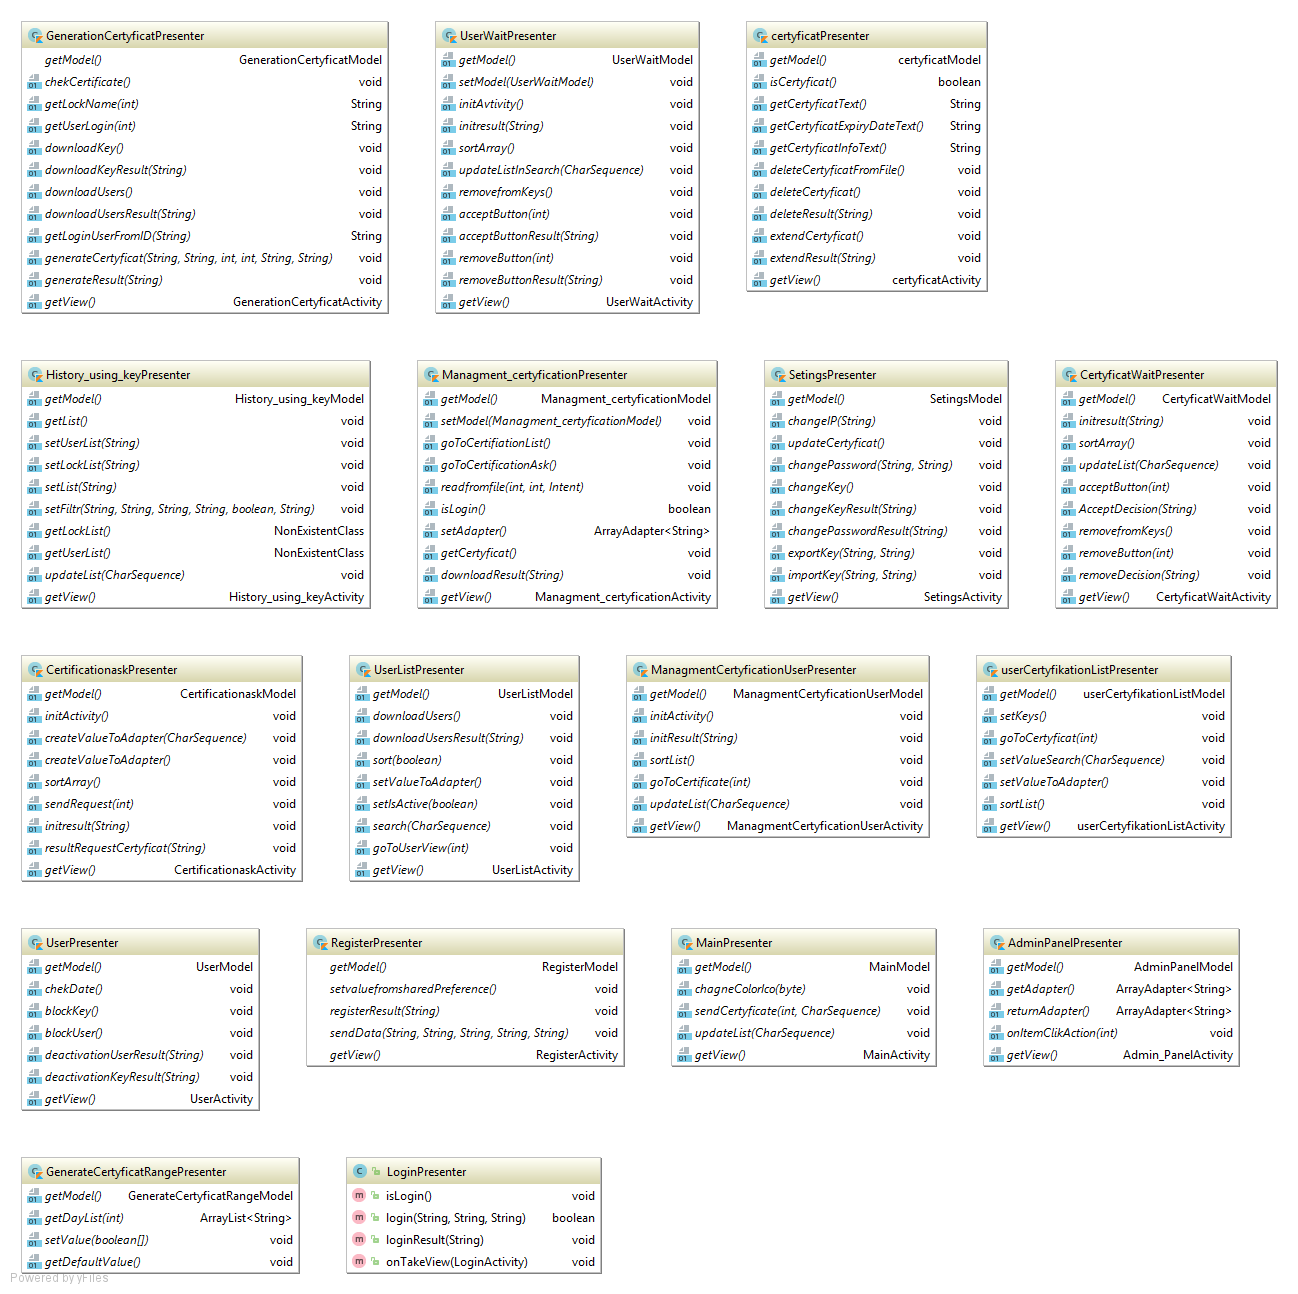
\includegraphics[width=16cm]{Obrazy/AM_DK_presenter}
\caption{Diagram klas dla paczki presenters}
\label{Diagram klas dla paczki presenters}
\end{figure}
\newpage

\paragraph*{Aplikacja serwera [Maciej Marciniak]}
Diagram klas znajdujący się na Rys. \ref{diagram:Diagram_klas_aplikacji_serwerowej} przedstawia klasy i metody potrzebne do realizacji projektu. Klasa Views przechowuje funkcje wykonujące akcje na bazie danych, zaś klasa URLs odpowiada za wskazanie pod jakim adresem URL znajduje się konkretna funkcja. Nazwy oraz budowę klas narzuca framework Django. Każda nazwa funkcji odpowiada nazwie URLa oraz opisuje jaką funkcję ma pełnić.

\paragraph*{Urządzenie sterujące [Maciej Marciniak]}
Zaprojektowane klasy, które mają zostać zaimplementowane w urządzeniu sterującym znajdują się \linebreak na~Rys.~\ref{diagram:Diagram_klas_urzadzenia_sterujacego}. Klasa Main jest głównym elementem programu. Ma być tutaj wywołana funkcja ''main'' (język Python nie wymaga funkcji niesocjalizującej charakterystycznej dla innych języków programowania). Obiekty klasy Certificate i CertificatePKI odpowiednio przechowywać mają dane certyfikatów dostępowych i szyfrujących. Metoda w Main Compare\_PKI\_Certificate porównywać ma klucze szyfrujące, czy są identyczne. Klasa Servo zarządzać ma fizycznym zamkiem przy drzwiach, uniwersalnie dla serwomechanizmu oraz elektrozamka. Funkcja Open ma mieć na celu ustawienie zamka w stanie otwartym, zaś Close analogicznie zamkniętym. 

\begin{figure}[!h]
\centering
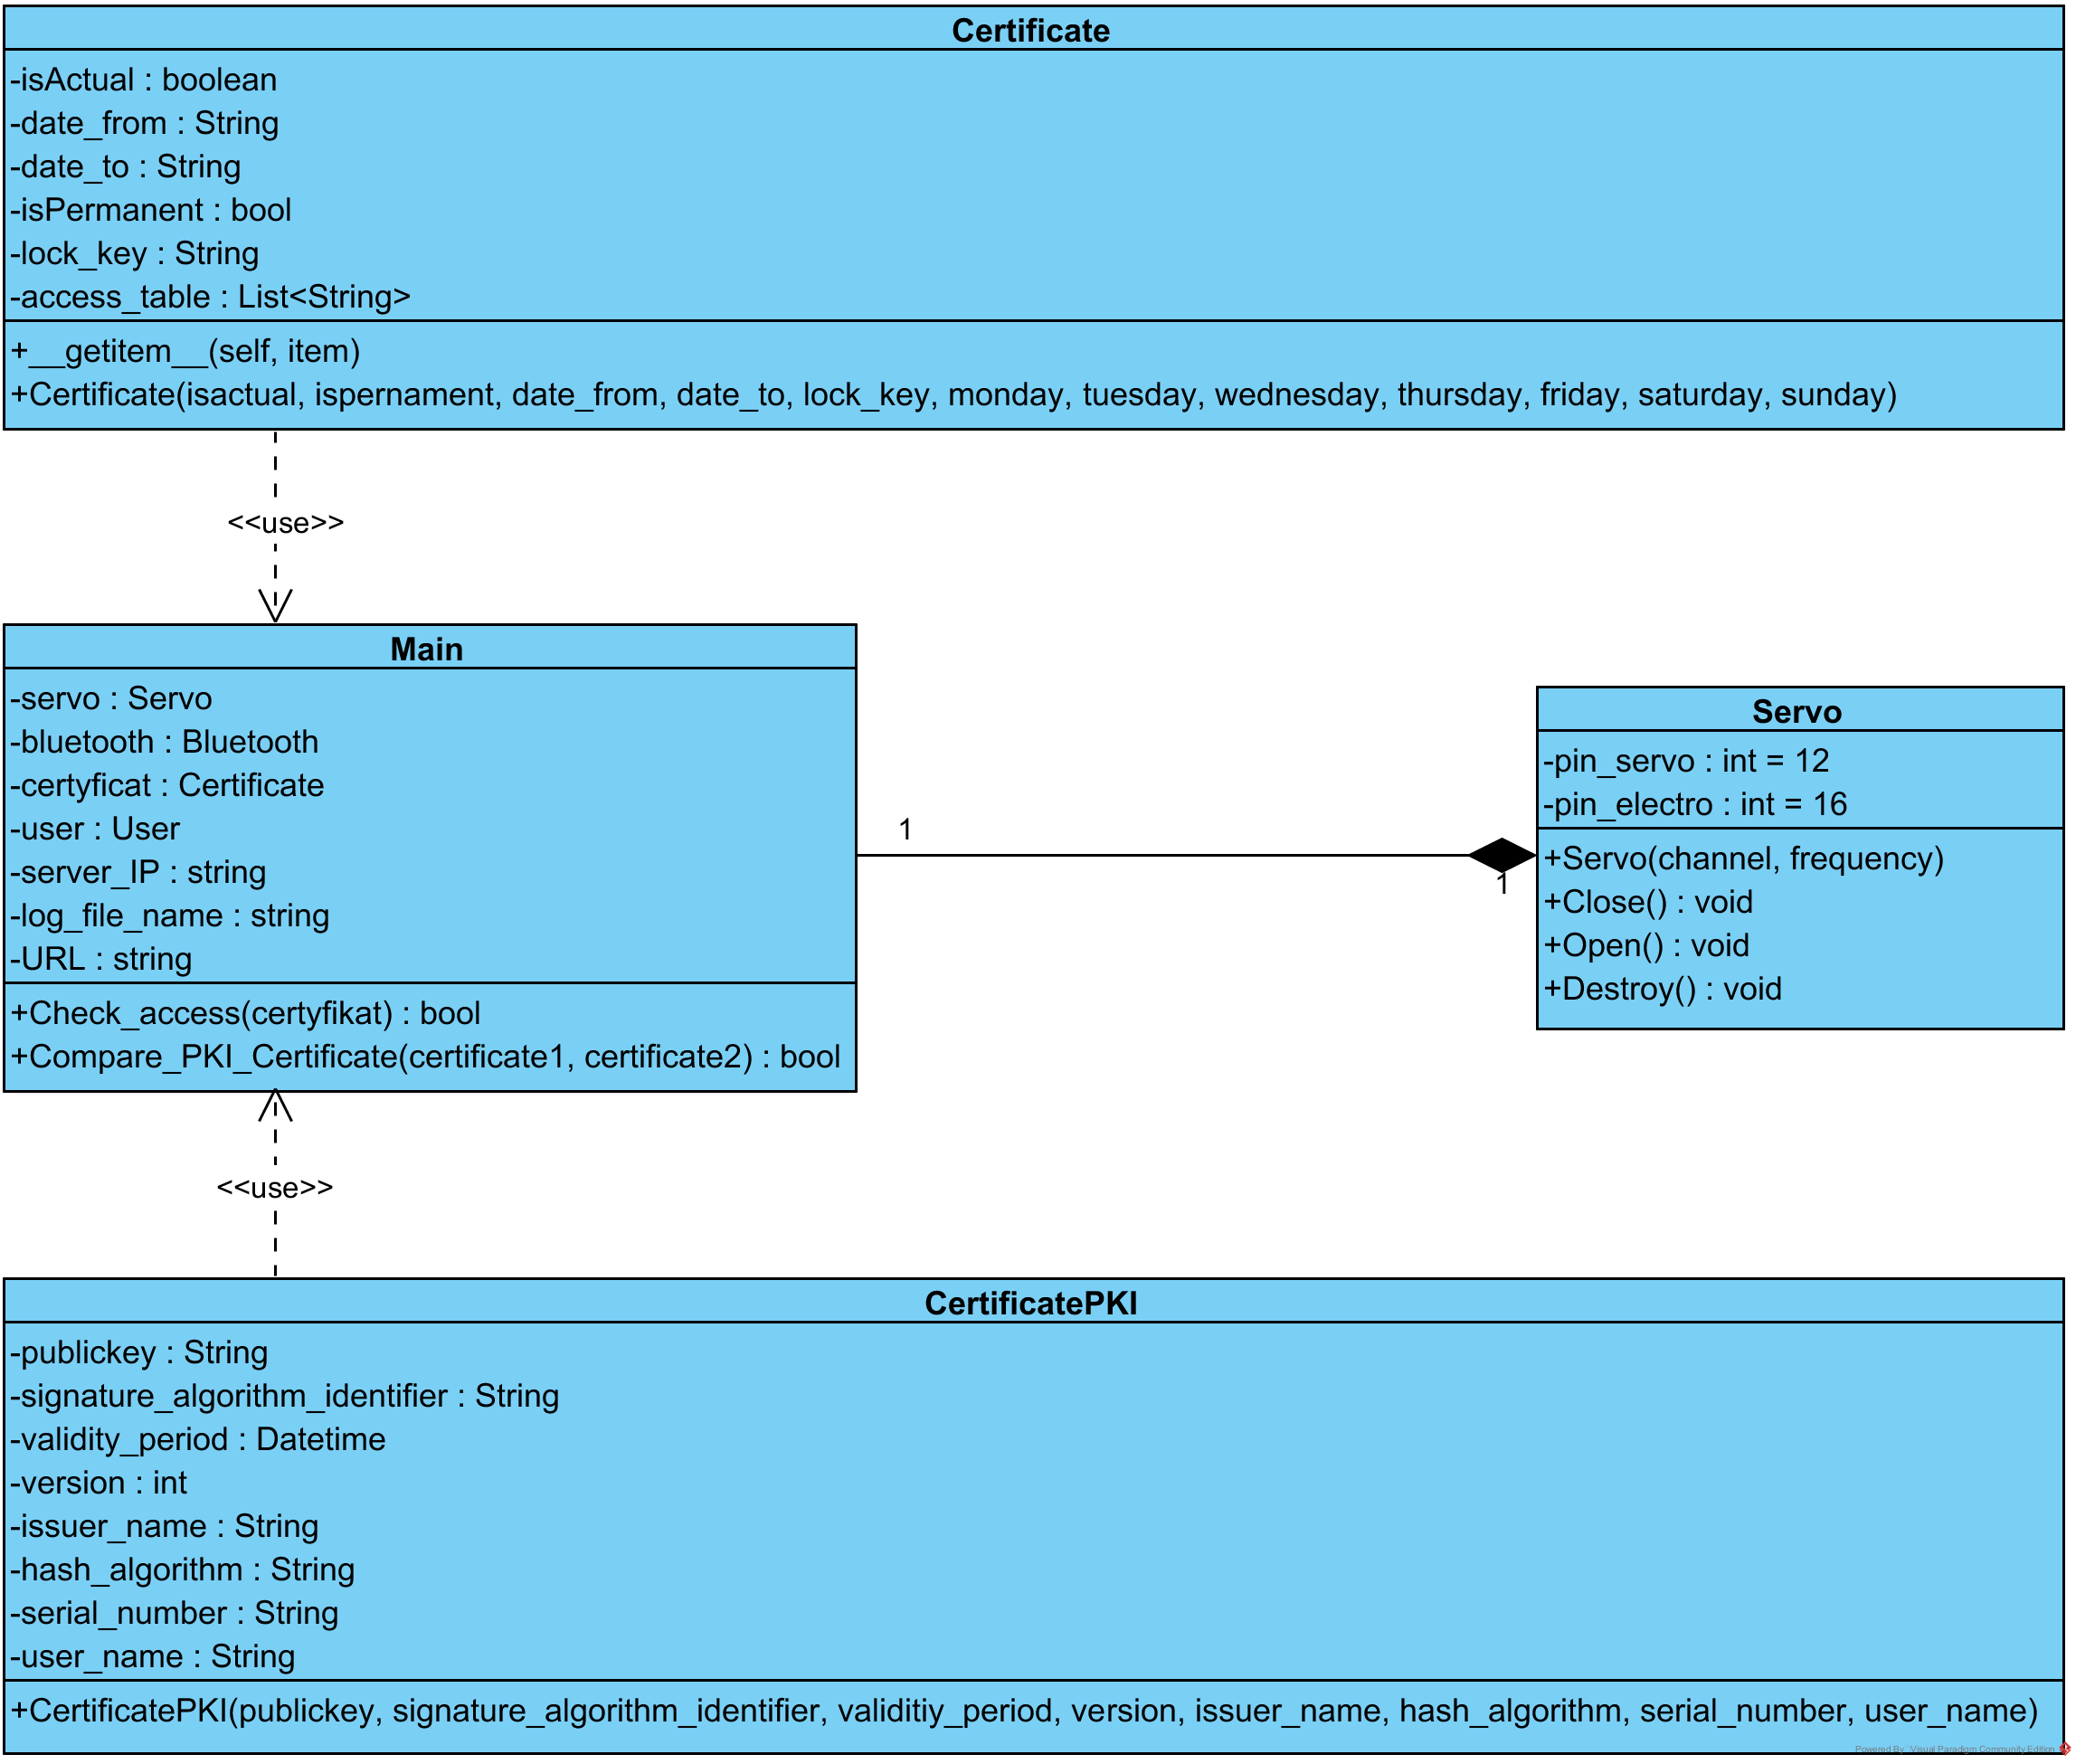
\includegraphics[width=16cm]{Obrazy/Diagram_klas_urzadzenie_sterujace.png}
\caption{Diagram klas urządzenia sterującego}
\label{diagram:Diagram_klas_urzadzenia_sterujacego}
\end{figure}

\begin{landscape}
\begin{figure}[!h]
\centering
\vspace{2.5cm}
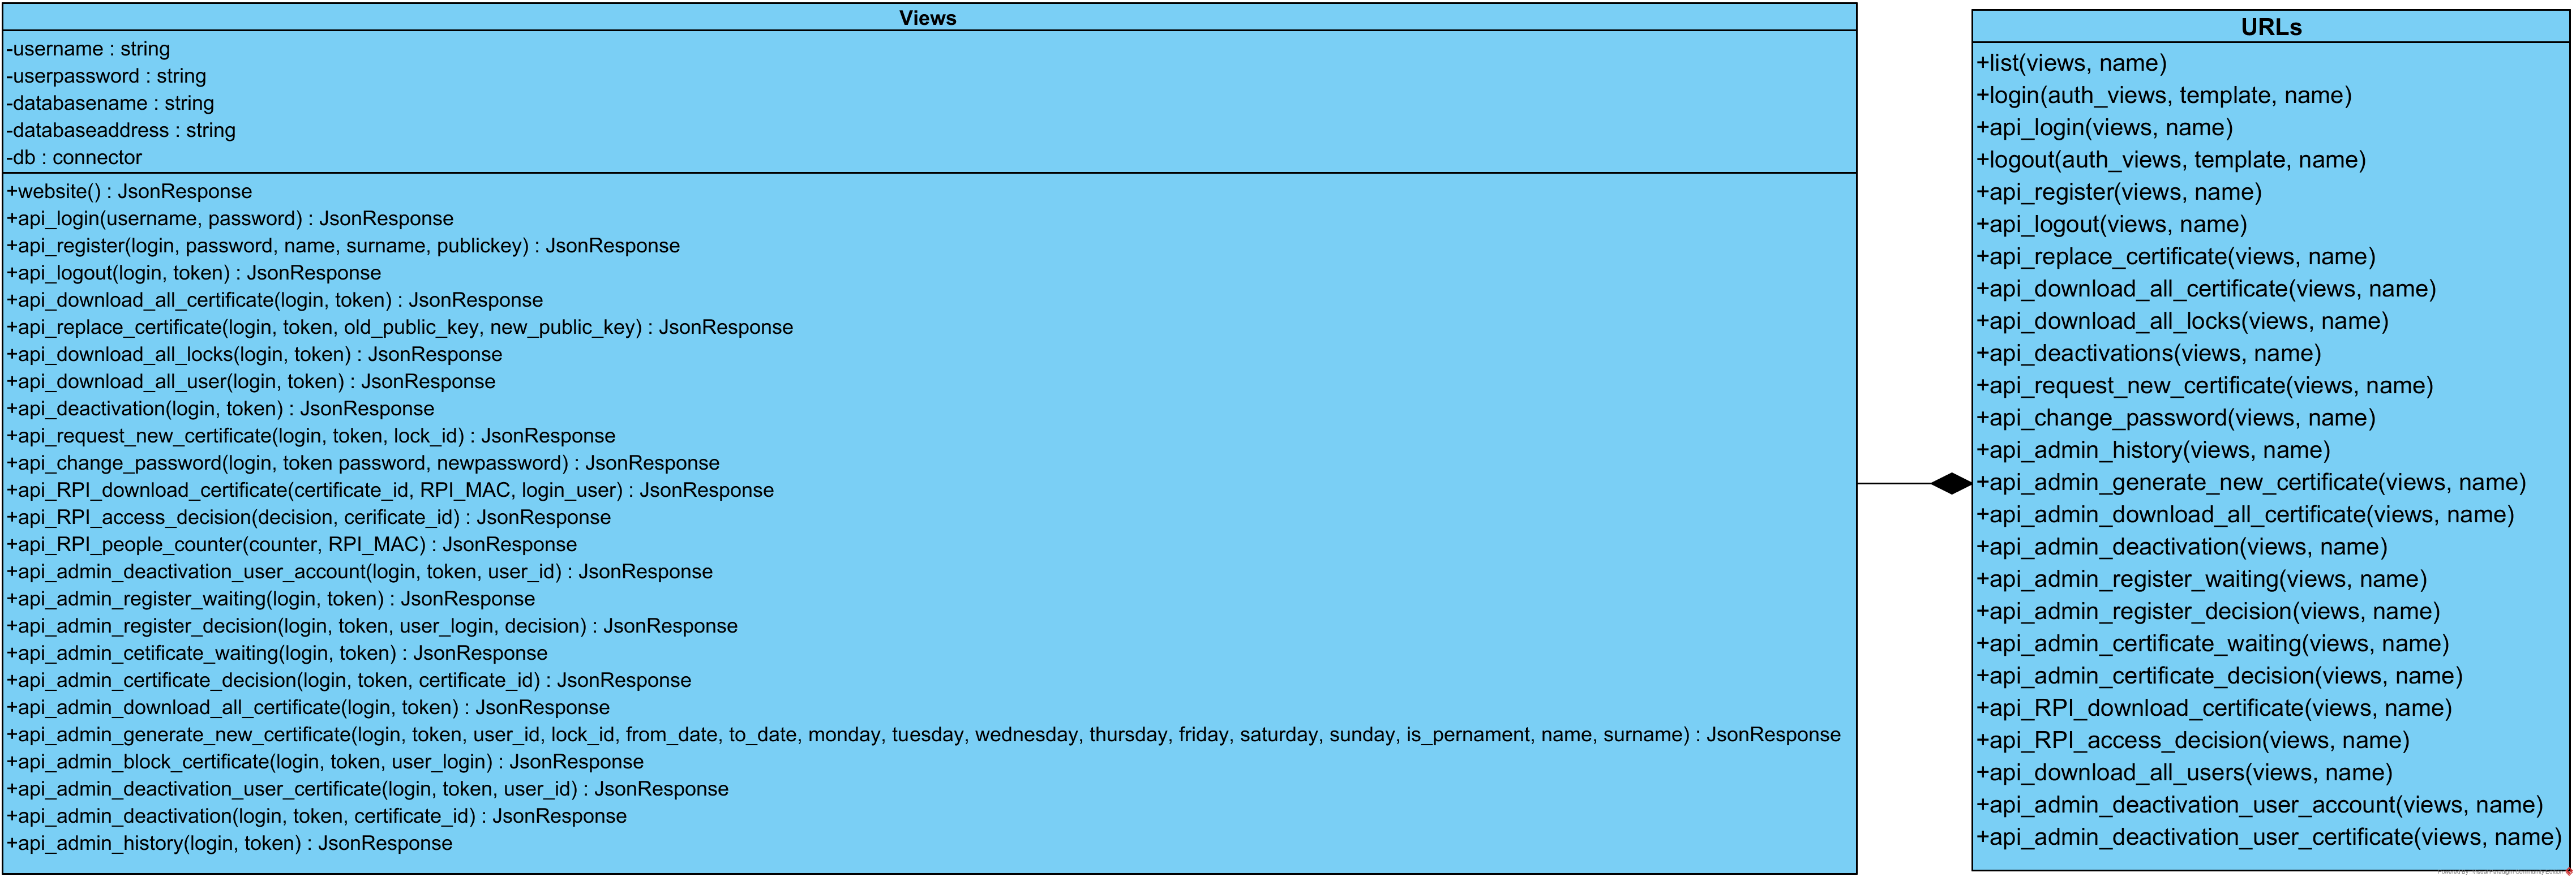
\includegraphics[width=24cm]{Obrazy/Diagram_klas_aplikacja_serwerowa.png}
\caption{Diagram klas aplikacji serwerowej}
\label{diagram:Diagram_klas_aplikacji_serwerowej}
\end{figure}
\end{landscape}

\paragraph*{Moduł zliczania osób [Maciej Marciniak]}
Moduł zliczania osób ze względu na swoją funkcjonalność i wykorzystanie biblioteki Open-CV nie wymaga tworzenia specjalnych klas, ani wyszczególnienia konkretnych metod. Jedyną możliwością jest wyodrębnienie klas, przechowujących zliczane osoby znajdujące się w obiektywie kamery. Klasa dla konkretnej osoby ma~posiadać metody do aktualizacji współrzędnych danej osoby oraz określające, czy przesuwa się w górę, czy w dół granicy obiektywu. Zmienne ''x'' i ''y'' przechowywać mają współrzędne osoby, ''donę'' oznaczać ukończenie śledzenia osoby, ''state'' obecny stan, a ''age'' i ''max\_age'' określać mają jak długo dany obiekt ma być namierzany.
\begin{figure}[!h]
\centering
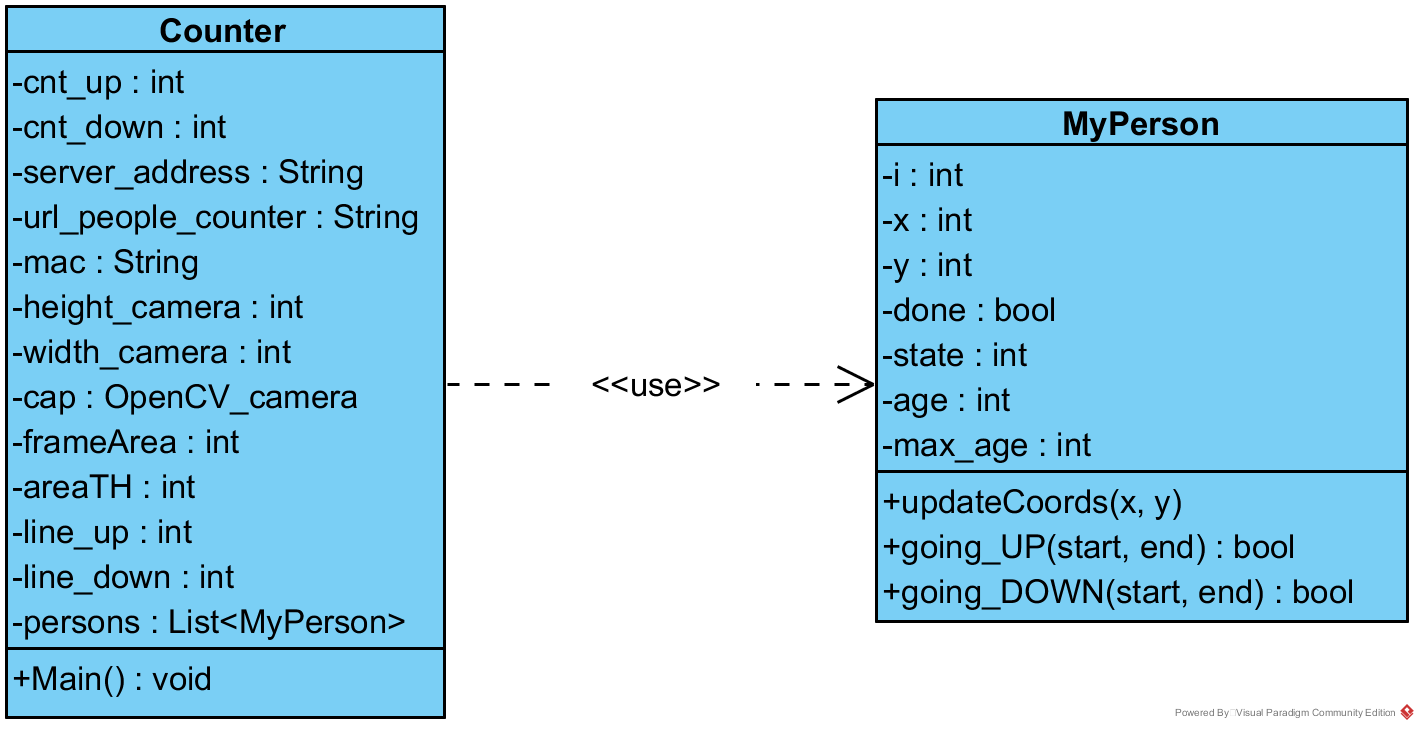
\includegraphics[width=12.5cm]{Obrazy/Diagram_klas_modul_zliczania_osob.png}
\caption{Diagram klas modułu zliczania osób}
\label{diagram:Diagram_klas_modul_zliczania_osob}
\end{figure}

\subsection{Schemat elektryczny systemu [Maciej Marciniak]}\label{sec:Schemat elektryczny zamka}
Urządzenie sterujące jest jedynym fizycznym elementem projektowanym w~tej~pracy  dyplomowej. Uproszczony schemat instalacji elektrycznej przedstawiony został na Rys. \ref{schemat:schemat elektryczny systemu}. Centrum modułu jest mikrokomputer \linebreak Raspberry Pi 3, zasilane z uniwersalnego gniazda USB. Zatem układ zasilany może być z komputera lub z zasilacza o napięciu 5V i minimalnym prądzie 1A. Urządzenie zostało zaprojektowane w taki sposób, aby można było podłączyć serwomechanizm i/lub elektrozamek. Umożliwia to dowolną konfigurację sprzętu według potrzeb i~możliwości danych drzwi. 

Zasilanie elektrozamka realizowane jest z zasilacza 12V będącego w stanie podać dużą wartość prądu. Wysokie wymagania związane są z trudem wprawienia zapadki elektrozamka w ruch, ponieważ w tego typu urządzeniach często znajdują się elektromagnesy niewielkich rozmiarów. Ze względu na wyższe napięcie zasilania zamka niż dostarczane przez Raspberry Pi, wymagane jest użycie tranzystora kluczującego prąd z zasilacza. Zdecydowano użyć elementu o oznaczeniu BD137-16 ze względu na swój niewielki koszt oraz wysoki prąd przewodzenia. Układ związany z serwomechanizmem jest zgodny z parametrami mikrokomputera, dlatego zasilanie oraz sterowanie prowadzone jest bezpośrednio z niego.

Piny sterujące urządzeniami w zamku są uzależnione od pełnionych w Raspberry Pi funkcji. Sterowanie elektrozamkiem możliwe jest przy użyciu niemal każdego pinu, ze względu na brak wymagań specjalistycznego sterowania, za to serwomechanizm wymaga zastosowania sygnału PWM, który musi być obsługiwany przez konkretny GPIO (w tym wypadku takim pinem jest GPIO\_18)\cite{RP3}.
\newpage
\begin{figure}[!h]
\centering
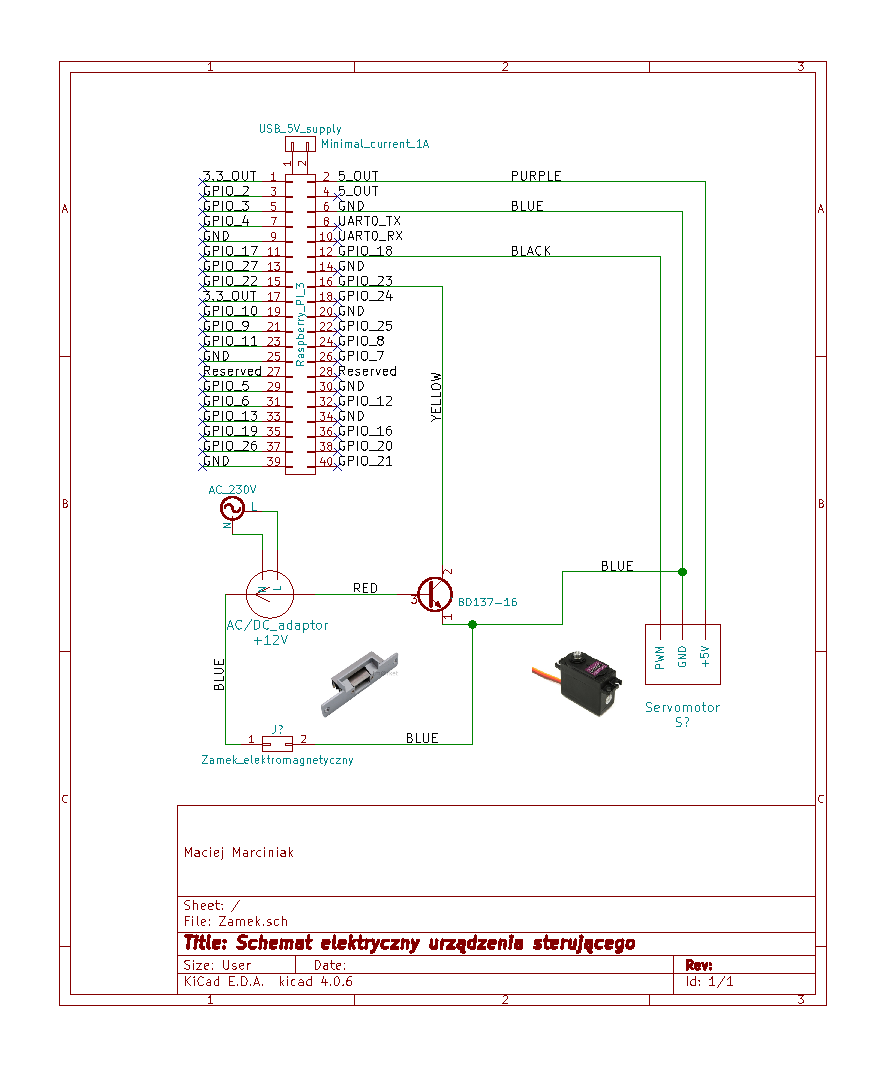
\includegraphics[width=17cm]{Obrazy/Schemat_elektryczny.pdf}
\caption{Schemat elektryczny systemu}
\label{schemat:schemat elektryczny systemu}
\end{figure}
\newpage

\subsection{Komunikacja modułów systemu z aplikacją  serwera [Maciej Marciniak]}\label{Komunikacja serwer}
Tworząc aplikację serwerową należy zapewnić możliwość komunikację (tak zwane API), która pozwoli na interakcję z zasobami zarządzanymi przez serwer. Przedstawiany system udostępniać powinien usługi dla~urządzenia sterującego, w~tym również modułu zliczającego osoby oraz dla aplikacji mobilnej. Ze względu na~odległości mogące dzielić systemy od siebie, zdecydowano, jako interfejs komunikacji sieć Internetową z użyciem bezpiecznego protokołu Https. 
\subsubsection{Komunikaty HTTPRequest pomiędzy urządzeniem sterującym a serwerem}
Komunikacja pomiędzy urządzeniem sterującym, a serwerem powinna  zapewniać możliwość weryfikacji poprawności certyfikatów dostępowych oraz szyfrujących w celu potwierdzenia tożsamości użytkownika oraz zdecydowaniu, czy dana osoba ma przydzielony dostęp do pomieszczenia o danej porze dnia. Dodatkowo serwer powinien udostępniać API do wpisywania liczby osób w~pomieszczeniu oraz wpisujące do bazy danych, czy dostęp został przyznany, czy nie. Wykaz wymaganych API znajduje się w Tabeli \ref{tab:http_raspberry}.
\subsubsection{Komunikaty HTTPRequest pomiędzy aplikacją mobilną a serwerem}
Aplikacja mobilna powinna posiadać podstawowe operacje użytkowników, takie jak logowanie, rejestracja, wylogowanie, dodatkowo powinny zostać udostępnione funkcje związane z zarządzaniem konta jak i certyfikatami dostępowymi. Funkcjonalności powiązane z operacjami na koncie to zmiana hasła, wymiana certyfikatu szyfrującego, możliwość blokowania konta. Funkcja zarządzającymi certyfikatami dostępowymi są generowanie nowych kluczy, blokowanie ich, aktywowanie. API powinno być dedykowane dla dwóch rodzajów użytkowników zwykłego oraz z uprawnieniami administratora. Właściwości funkcji drugiego typu konta powinny dodatkowo udostępniać podgląd w historię używania poszczególnych zamków oraz edycję wszystkich parametrów kont użytkownika zwykłego. Wykaz zaprojektowanego API znajduje się w Tabeli \ref{tab:http_mobilne}\cite{programowanie_aplikacji_webowych}.
\begin{longtable}[!ht]{|m{4cm}|m{4.5cm}|m{3.9cm}|m{2.8cm}|} 
\caption{Tabela komunikatów HTTP dla Raspberry Pi}
\label{tab:http_raspberry}\\
\hline
Adres URL & Parametry & Odpowiedź & Opis \\ \hline
/api/RPI/download/\-certificate/ & certificate\_id --- identyfikator certyfikatu, \newline RPI\_MAC --- adres MAC urządzenia, \newline login\_user --- login użytkownika & ''data'': dict\_all\_certificate, \newline ''public\_key'': public\_key \tablinia ''data'': ''invalid'' & Pobranie certyfikatu użytkownika \\ \hline
/api/RPI/access\_decision/ & certificate\_id --- identyfikator certyfikatu \newline decision --- informacja o odmowie/akceptacji dostępu & ''status'': ''ok'' \tablinia ''data'': ''invalid'' & Informacja do serwera o statusie otwierania zamka \\ \hline
/api/RPI/people\_counter/ & counter --- liczba osób w pomieszczeniu, \newline RPI\_MAC --- adres MAC urządzenia & ''status'': ''ok'' \tablinia ''data'': ''Invalid'' & Ustawienie licznika osób w pomieszczeniu \\ \hline
\end{longtable}

\begin{landscape}
\begin{longtable}[!ht]{|m{5cm}|m{6.5cm}|m{5cm}|m{5.5cm}|} 
\caption{Tabela komunikatów HTTP dla urządzenia mobilnego}
\label{tab:http_mobilne}\\
\hline
Adres URL & Parametry & Odpowiedź & Opis \\ \hline
/api/login/ & username --- login użytkownika, \newline password --- hasło użytkownika & ''status'': ''ok'', ''token'': token \tablinia ''status'':''ERROR~\mbox{PASSWORD}'', ''token'': ''invalid'' \tablinia ''status'': ''not activated'', \newline ''token'': ''invalid'', \tablinia ''status'': ''blocked'', \newline''token'': ''invalid'' & Logowanie użytkownika do aplikacji \\ \hline
/api/register/ & login --- login użytkownika, \newline password --- hasła użytkownika, \newline name --- imię użytkownika, \newline surname -- nazwisko użytkownika, \newline publickey --- klucz publiczny użytkownika & ''status'': 'ERROR'' \tablinia ''status'': ''REGISTER OK'' & Rejestracja nowego użytkownika do aplikacji \\ \hline
/api/logout/ & login --- login użytkownika, \newline token --- klucz sesji logowania & ''status'': ''logout'' \tablinia ''status'': ''invalid'' & Wylogowanie użytkownika z aplikacji \\ \hline
/api/download/all\_certifacate/ & login --- login użytkownika, \newline token --- klucz sesji logowania & ''data'': dict\_all\_certificate \tablinia ''status'': ''invalid'' & Pobranie wszystkich dostępnych certyfikatów użytkownika \\ \hline
/api/download/all\_locks/ & login --- login użytkownika, \newline token --- klucz sesji logowania & ''data'': dict\_all\_locks \tablinia ''status'': ''invalid'' & Pobranie listy wszystkich dostępnych zamków w systemie \\ \hline
/api/download/all\_user/ & login --- login użytkownika, \newline token --- klucz sesji logowania & ''data'': dict\_all\_users \tablinia ''status'': ''invalid'' & Pobranie listy wszystkich użytkowników systemu \\ \hline
/api/deactivation/ & login --- login użytkownika, \newline token --- klucz sesji logowania, \newline certificate\_id --- identyfikator certyfikatu do usunięcia & ''status'': ''ok'' \tablinia ''status'': ''invalid'' & Usunięcie dostępu do certyfikatu \\ \hline
/api/request\_new\_certificate/ & login --- login użytkownika, \newline token --- klucz sesji logowania, \newline lock\_id --- identyfikator zamka & ''status'': ''ok'' \tablinia ''status'': ''invalid'' & Wnioskowanie o nowy certyfikat \\ \hline
/api/change\_password/ & login --- login użytkownika, \newline token --- klucz sesji logowania, \newline newpasswd --- nowe hasło użytkownika & ''status'': ''ok'' \tablinia ''status'': ''invalid'' & Zmiana hasła użytkownika \\ \hline
/api/replace\_certificate/ & login --- login użytkownika, \newline token --- klucz sesji logowania, \newline old\_public\_key --- obecny klucz publiczny użytkownika, \newline new\_public\_key --- nowy klucz publiczny użytkownika & ''status'': ''ok'', \newline ''data'': dict\_certificate \tablinia ''status'': ''invalid'' & Wymiana certyfikatu szyfrującego na żądanie użytkownika \\ \hline
/api/admin/history/ & login --- login użytkownika, \newline token --- klucz sesji logowania & ''data'': dict\_history \tablinia ''status'': ''invalid'' & Pobranie historii użycia zamków w systemie (administrator) \\ \hline
/api/admin/download/\linebreak all\_certificate/ & login --- login użytkownika, \newline token --- klucz sesji logowania & ''data'': dict\_all\_certificate \tablinia ''status'': ''invalid'' & Pobranie wszystkich certyfikatów z systemu (administrator)\\ \hline
/api/admin/deactivation/ & login --- login użytkownika, \newline token --- klucz sesji logowania, \newline certificate\_id --- identyfikator certyfikatu do usunięcia & ''status'': ''ok'' \tablinia ''status'': ''invalid'' & Usunięcie dostępu do certyfikatu (administrator) \\ \hline
/api/admin/register\_waiting/ & login --- login użytkownika, \newline token --- klucz sesji logowania & ''status'': ''ok'' \tablinia ''status'': ''invalid'' & Pobranie listy oczekujących użytkowników na zaakceptowanie rejestracji \\ \hline
/api/admin/register\_decision/ & login --- login użytkownika, \newline token --- klucz sesji logowania, \newline user\_login --- login użytkownika, którego dotyczy decyzja, \newline decision --- decyzja True/False dotycząca akceptacji rejestracji & ''status'': ''ok'' \tablinia ''status'': ''invalid'' & Podjęcie decyzji przez administratora dotycząca rejestracji użytkownika o danym loginie \\ \hline
/api/admin/certificate\_waiting/ & login --- login użytkownika, \newline token --- klucz sesji logowania & ''status'': ''ok'' \tablinia ''status'': ''invalid'' & Pobranie listy oczekujących certyfikatów na zaakceptowanie \\ \hline
/api/admin/certificate\_decision/ & login --- login użytkownika, \newline token --- klucz sesji logowania, \newline certificate\_id --- identyfikator certyfikatu, którego dotyczy decyzja & ''status'': ''ok'' \tablinia ''status'': ''invalid'' & Podjęcie decyzji przez administratora dotycząca przyjęcia \\ \hline
/api/admin/\-generate\_new\_certificate/ & login --- login użytkownika, \newline token --- klucz sesji logowania, \newline user\_id --- identyfikator użytkownika, \newline lock\_id --- identyfikator zamka, \newline from\_date --- data od której obowiązuje certyfikat, \newline to\_date --- data do której obowiązuje certyfikat, \newline monday...sunday --- 7 parametrów oznaczjacych zakresy godzin w poszczególnych dniach tygodnia, \newline is\_pernament --- czy dostęp jest ciągły, \newline name --- imię użytkownika certyfikatu, \newline surname --- nazwisko użytkownika certyfikatu & ''status'': ''ok'' \tablinia ''status'': ''invalid'' & Generowanie nowego certyfikatu (administrator) \\ \hline
/api/admin/\-deactivation\_user\_accout/ & login --- login użytkownika, \newline token --- klucz sesji logowania, \newline user\_id --- identyfikator użytkownika, którego konto ma zostać zablokowane & ''status'': ''ok'' \tablinia ''status'': ''invalid'' & Zablokowanie konta wybranego użytkownika (administrator) \\ \hline
/api/admin/deactivation\-\_user\_certificate/ & login --- login użytkownika, \newline token --- klucz sesji logowania, \newline user\_id --- identyfikator użytkownika, którego certyfikat szyfrujący ma zostać zablokowany & ''status'': ''ok'' \tablinia ''status'': ''invalid'' & Zablokowanie certyfikatu szyfrującego wybranego użytkownika (administrator) \\ \hline
\end{longtable}
\end{landscape}
\newpage
\subsection{Interfejs komunikacji pomiędzy urządzeniem sterującym i aplikacją mobilną [Maciej Marciniak]}
W rozdziale \ref{Komunikacja serwer} opisano dwie ścieżki komunikacji urządzeń z serwerem, trzecią opcją jest komunikacja pomiędzy urządzeniem sterującym, a aplikacją mobilną. W tym wypadku nie jest istotna duża odległość komunikacji, wręcz jest niewskazana. Odpowiednim interfejsem, zapewniającym szybką i uniwersalną transmisję jest moduł bluetooth, w który wersja mikrokomputera Raspberry Pi 3 jest wyposażona. 

Komunikacja pomiędzy urządzeniami polega tylko na przesyle podpisanych cyfrowo certyfikatów dostępowych. Format przesyłanych danych jest w postaci: \\
\begin{minipage}[t]{8cm}
<id~certyfikatu>;\\<login~użytkownika>;\\<sygnatura~klucza~dostępowego>;\\<certyfikat~szyfrujący~w~postaci~JSONa>
\end{minipage} 

\subsection{Interfejs graficzny systemu [Damian Filipowicz]}\label{sec:Projekt interfejsu graficznego}
Jednym z dwóch modułów posiadających w systemie interfejs graficzny jest aplikacja mobilna, drugim zaś strona internetowa. Aplikacja mobilna zawierać powinna wszystkie funkcjonalności systemu z wykorzystaniem czytelnego interfejsu użytkownika. Strona internetowa  ma mieć na celu interakcję tylko z administratorem systemu, dlatego nie są stawiany wysoki priorytet estetyczny. Nominalną wielkością ekranu braną pod uwagę przy projektowaniu interfejsu graficznego dla aplikacji mobilnej będzie ekran o wielkości 5 in. Motywacją takiego wyboru jest rozkład popularności ekranów dla urządzeń mobilnych w 2017 roku. Jak widać na załączonym rysunku (rys. \ref{rys:prognoza}) wielkość ekranu 5,0 jest pierwszą znaczącą wielkością dla urządzeń mobilnych.
\begin{figure}[ht!]
\centering
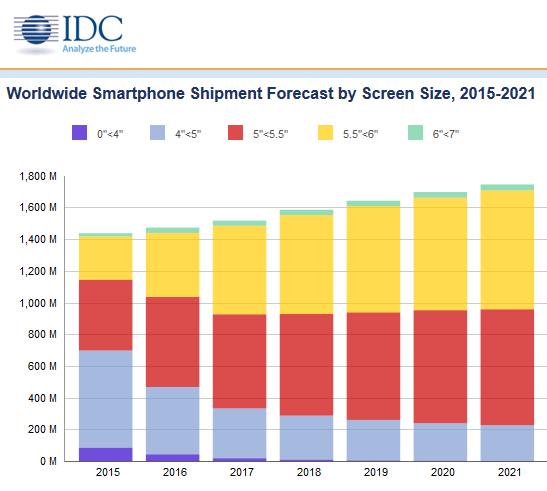
\includegraphics[width=13cm]{Obrazy/porowananie}
\caption{Prognoza trendów wielkości ekranów dla urządzeń mobilnych na przestrzeni lat 2015-2021\cite{Prognoza android}}
\label{rys:prognoza}
\end{figure}

\subsubsection{Widoki aplikacji mobilnej}
\paragraph*{Panel logowania użytkownika}
Widok umożliwiać będzie zalogowanie się użytkownika do systemu poprzez podanie loginu, hasła oraz adres IP serwera w odpowiednie pola, a następnie kliknięcie w przycisk ''ZALOGUJ SIĘ”. Samo pole hasła będzie maskowane. Jeśli nie posiada się konta, zostanie utworzona możliwość  utworzenia konta poprzez przycisk ''ZAREJESTRUJ SIĘ”. (Rys. \ref{rys:panel_logowania_pionowo})

\begin{figure}[ht!]
\begin{minipage}{0.45\textwidth}
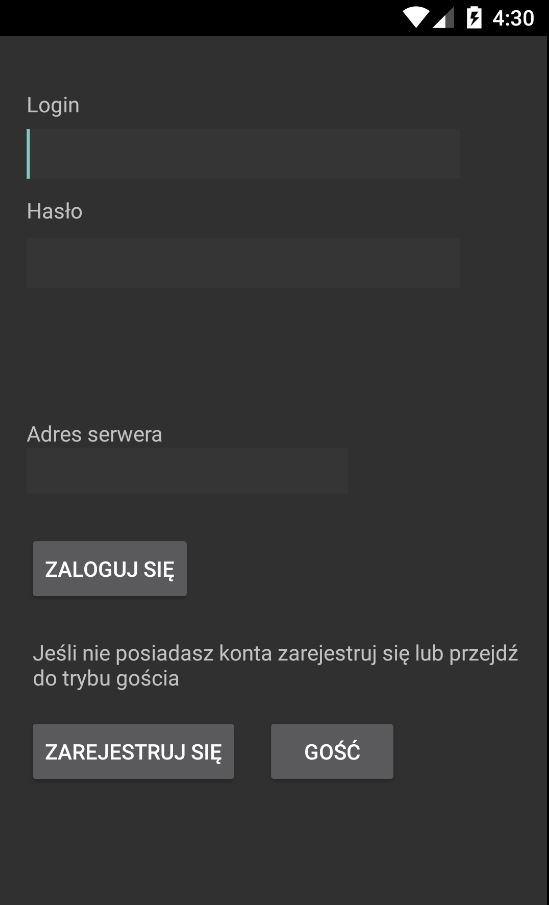
\includegraphics[width=\textwidth]
{Obrazy/logowanie_uzytkownika_pionowo}
\caption{Panel logowania użytkownika}
\label{rys:panel_logowania_pionowo}
\end{minipage}
\hspace{0.1\textwidth}
\begin{minipage}{0.45\textwidth}
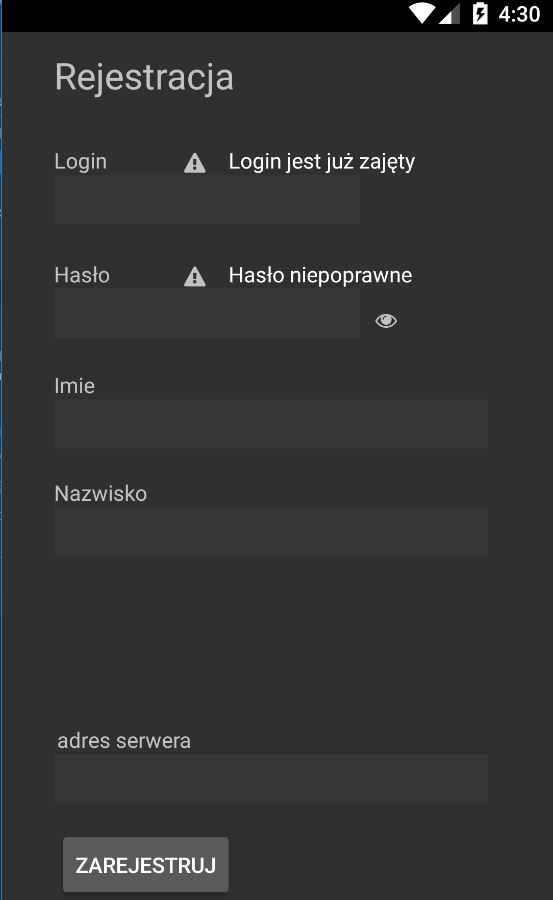
\includegraphics[width=\textwidth]{Obrazy/rejestracja_uzytkownika_pionowo}
\caption{Panel logowania użytkownika }
\label{rys:panel_rejestracji_pionowo}
\end{minipage}
\end{figure}

\paragraph*{Panel rejestracji użytkownika}
Panel rejestracji służyć będzie do utworzenie nowego użytkownika poprzez podanie loginu, hasła, imienia i nazwiska użytkownika oraz adresu IP serwera do którego chcemy się zarejestrować. Pole z hasłem będzie maskowane wraz z możliwością odkrywania hasła przy pomocy ikonki oko Po upewnieniu się, że wszystkie dane są poprawne, aby zakończyć proces rejestracji, trzeba będzie kliknąć przycisk ''ZAREJESTRUJ”. (Rys. \ref{rys:panel_rejestracji_pionowo})

\newpage
\paragraph*{Panel listy zamków}
Widok listy dostępnych zamków przedstawia listę nazw zamków do jakich dany użytkownik ma dostęp. Ułatwieniem będzie możliwość sortowania wyników i wyszukiwanie po nazwach. Kliknięcie w nazwę zamka spowoduje otwarcie zamka. Zmiana koloru\footnote{ Opisy znaczeń poszczególnych kolorów oraz symboli opisane są w rozdziale \ref{Symbolika ikon}} ikon zamków sygnalizować będzie status zamka. (Rys. \ref{rys:panel_listy_dostepnych_zamkow_pionowo})

\begin{figure}[ht!]
\begin{minipage}{0.45\textwidth}
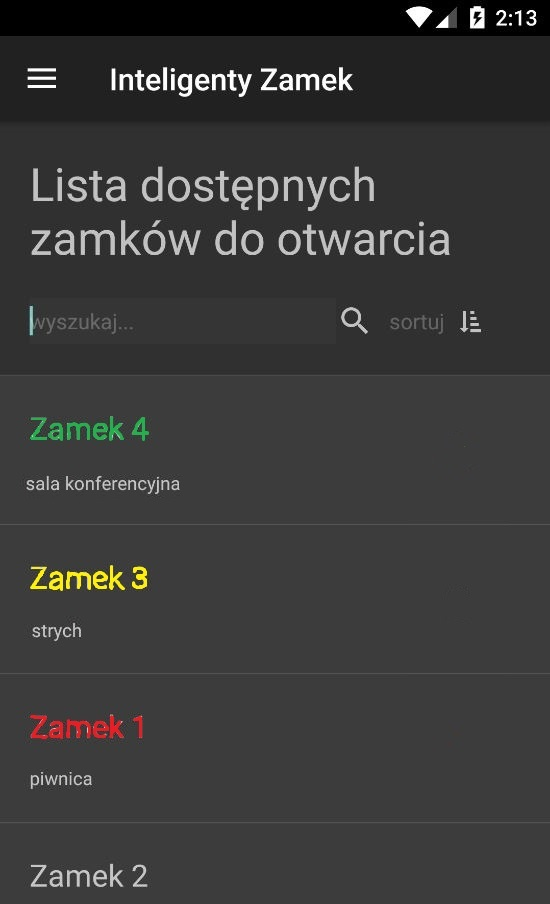
\includegraphics[width=\textwidth]
{Obrazy/lista_dostepnych_zamkow_pionowo}
\caption{Lista dostępnych zamków}
\label{rys:panel_listy_dostepnych_zamkow_pionowo}
\end{minipage}
\hspace{0.1\textwidth}
\begin{minipage}{0.45\textwidth}
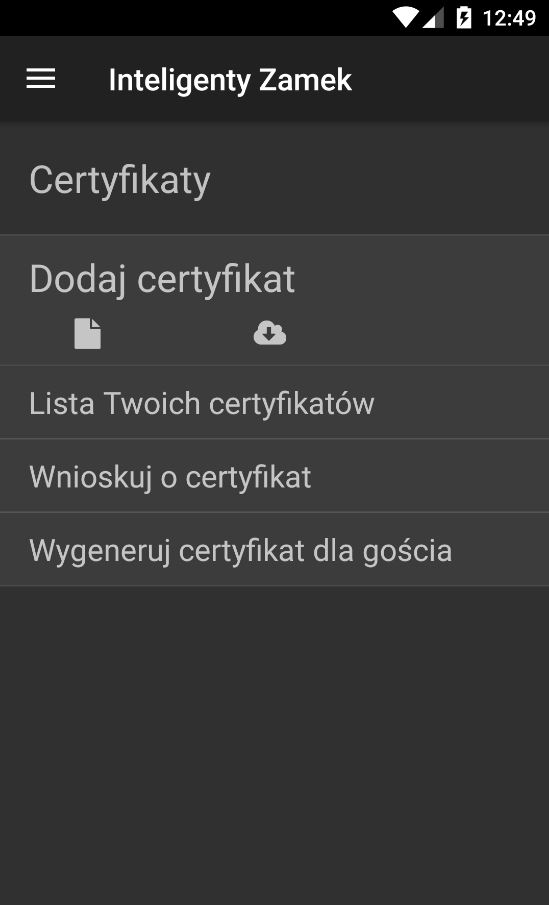
\includegraphics[width=\textwidth]{Obrazy/zarzadzaj_certyfikatami_pionowo}
\caption{Panel zarządzania certyfikatami }
\label{rys:panel_zarządzania_certyfikatami_pionowo}
\end{minipage}
\end{figure}

\paragraph*{Panel zarządzania certyfikatami}
Panel zarządzania certyfikatami umożliwi wybór funkcji dodania certyfikatu. Kolejne pozycje to lista posiadanych certyfikatów oraz wysłanie wniosku o utworzenie nowego certyfikatu  (Rys. \ref{rys:panel_zarządzania_certyfikatami_pionowo})
\newpage

\paragraph*{Panel boczny}
Panel boczny pozwalać będzie na szybkie przełączanie pomiędzy widokami. Chowany zostanie po lewej stronie ekranu. Umożliwi przechodzenie odpowiednio do listy zamków, zarządzania certyfikatami, panelu administracyjnego oraz ustawień. Ostatnia pozycja spowoduje wylogowanie z aplikacji. Pnanel ten w zależnośći od uprawnień użytkownika możę posiadać lub nie pole z panelem administraotra (Rys. \ref{rys:panel_boczny_pionowo} i \ref{rys:panel_boczny_pionowo2})

\begin{figure}[ht!]
\begin{minipage}{0.45\textwidth}
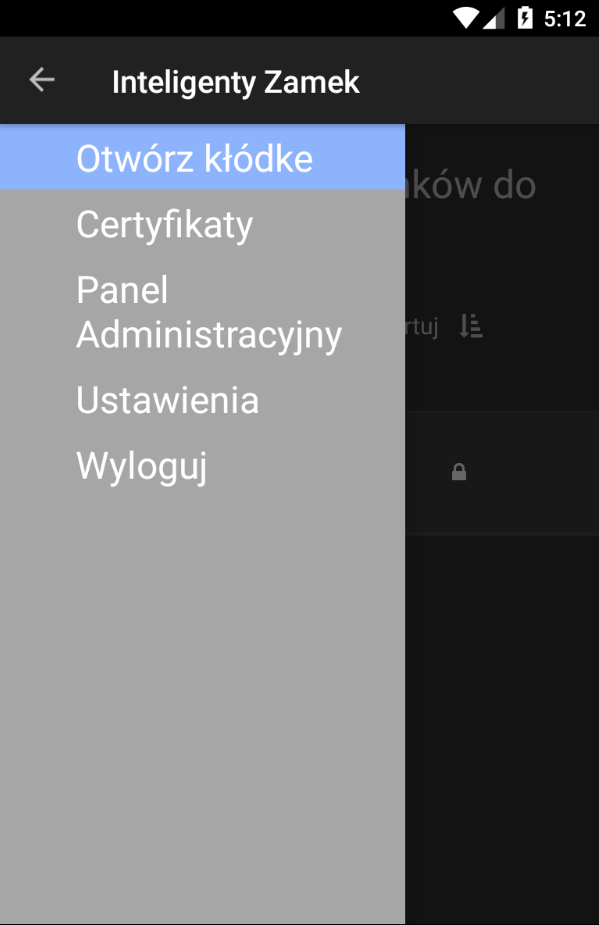
\includegraphics[width=\textwidth]
{Obrazy/panel_boczny_pionowo}
\caption{Panel boczny z uprawnieniami administratora}
\label{rys:panel_boczny_pionowo}
\end{minipage}
\hspace{0.1\textwidth}
\begin{minipage}{0.45\textwidth}
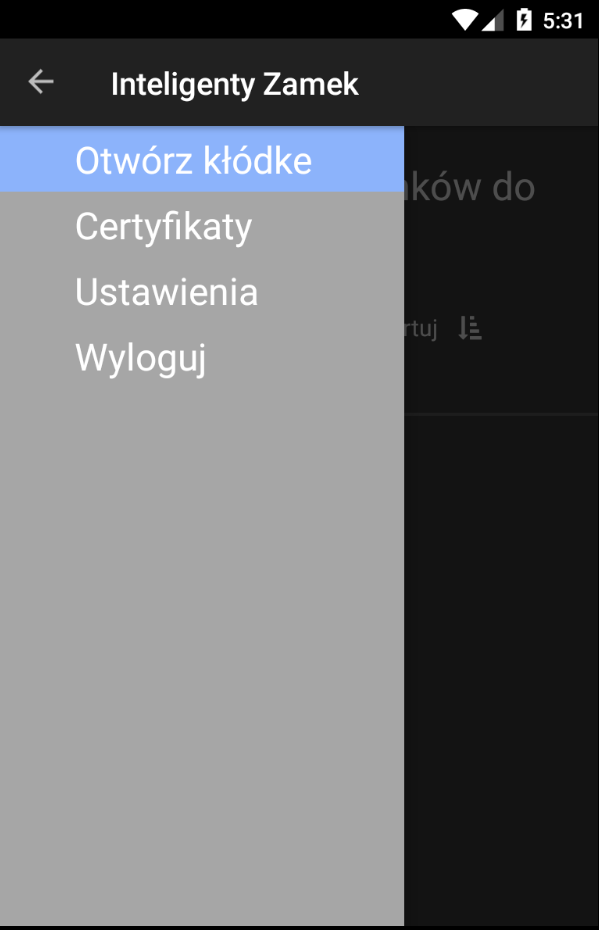
\includegraphics[width=\textwidth]{Obrazy/panel_boczny_pionowo2}
\caption{Panel boczny bez uprawnieni administratora}
\label{rys:panel_boczny_pionowo2}
\end{minipage}
\end{figure}
\newpage

\paragraph*{Panel listy certyfikatów}
Panel listy certyfikatów, będzie listą aktualnych certyfikatów należących do użytkownika. Kliknięcie w dany certyfikat przeniesie do widoku szczegółowego związanego z operacjami na tym certyfikacie. (Rys. \ref{rys:panel_listy_certyfikatów_pionowo} )

\begin{figure}[ht!]
\begin{minipage}{0.45\textwidth}
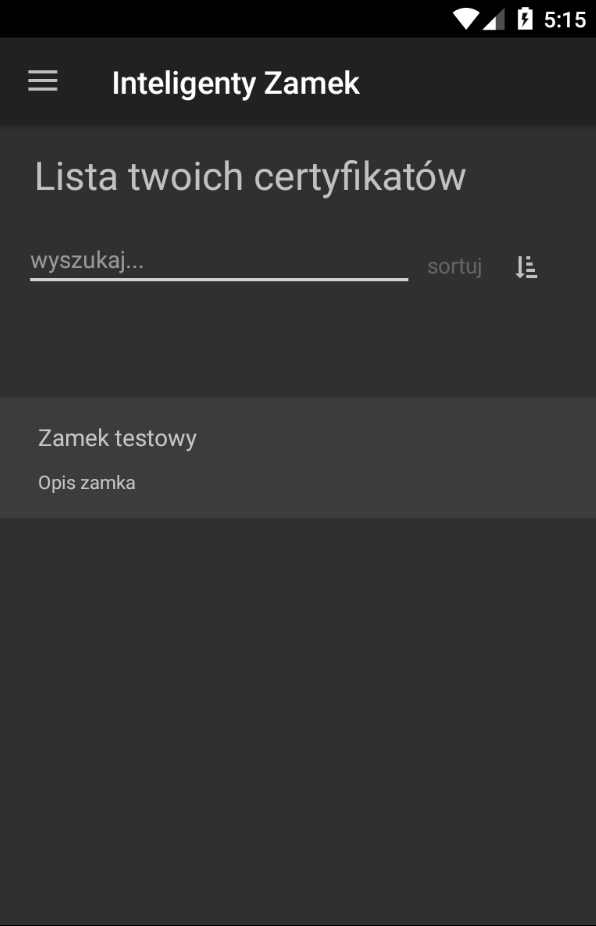
\includegraphics[width=\textwidth]
{Obrazy/lista_certyfikatow_pionowo}
\caption{Panel listy certyfikatów}
\label{rys:panel_listy_certyfikatów_pionowo}
\end{minipage}
\hspace{0.1\textwidth}
\begin{minipage}{0.45\textwidth}
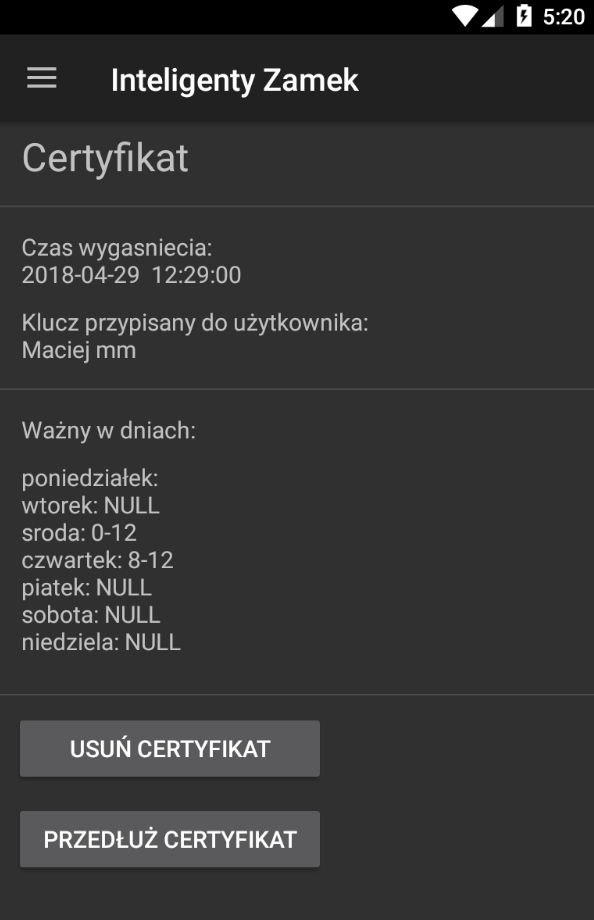
\includegraphics[width=\textwidth]{Obrazy/certyfikat_pionowo}
\caption{Panel certyfikatu }
\label{rys:panel_certyfikatu_pionowo}
\end{minipage}
\end{figure}

\paragraph*{Panel certyfikatu}
Panel certyfikatu zawierać będzie informacje o dacie wygaśnięcia, którego zamku dotyczy oraz w jakim czasie przyznaje dostęp. Na dole dostępne będą dwa przyciski pozwalające usunąć certyfikat lub wysłać prośbę o~przedłużenie ważności. W zależności od tego, czy użytkownik ma uprawnienia administratora przycisk przedłuż certyfikat albo wyśle zgłoszenie do serwera (dla użytkownika bez uprawnieni administratora) albo przeniesie do~panelu generowania certyfikatu (dla użytkownika o uprawnieniach administratora) (Rys. \ref{rys:panel_certyfikatu_pionowo})
\newpage

\paragraph*{Panel wnioskowania o certyfikat}
Panel wnioskowania o certyfikat polegać będzie na wybraniu z listy wszystkich zamków, konkretnego do~którego chcemy uzyskać dostęp i wysłaniu wniosku o przydzielenie dostępu. (Rys. \ref{rys:panel_wnioskowania_o_certyfikat_pionowo})

\begin{figure}[ht!]
\begin{minipage}{0.45\textwidth}
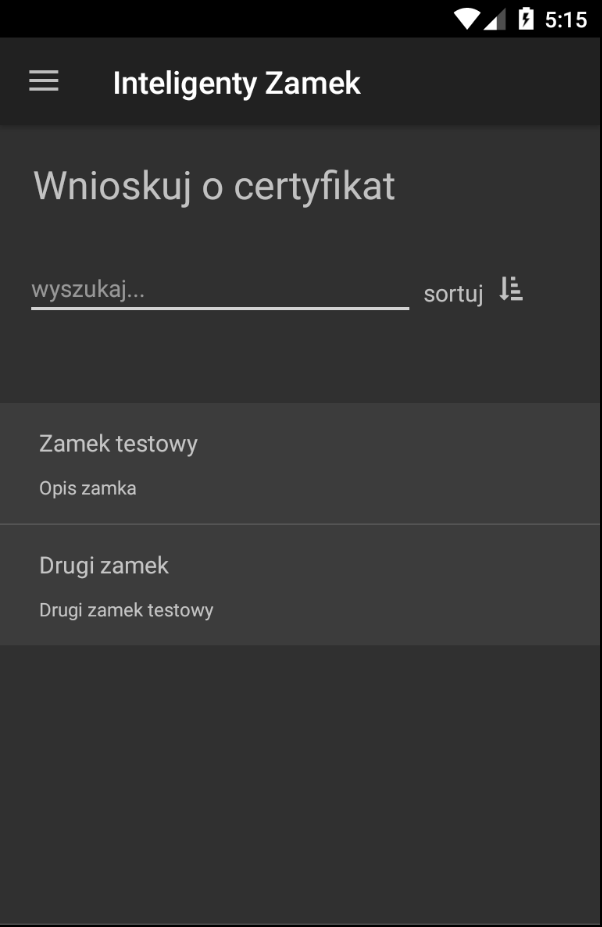
\includegraphics[width=\textwidth]
{Obrazy/wnioskuj_o_certyfikat_pionowo}
\caption{Panel wnioskowania o certyfikat }
\label{rys:panel_wnioskowania_o_certyfikat_pionowo}
\end{minipage}
\hspace{0.1\textwidth}
\begin{minipage}{0.45\textwidth}
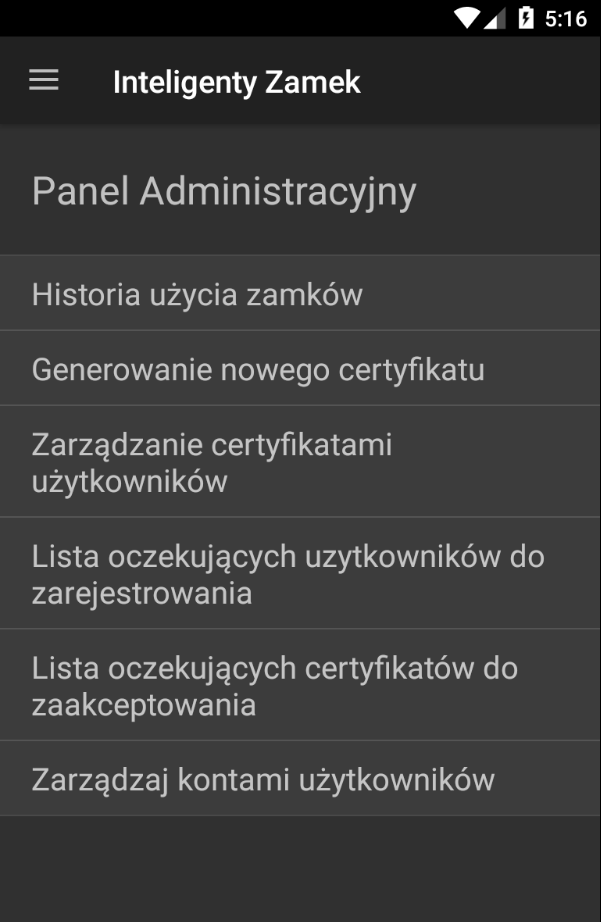
\includegraphics[width=\textwidth]{Obrazy/panel_administracyjny_pionowo}
\caption{Panel administratora}
\label{rys:panel_administracyjny_pionowo}
\end{minipage}
\end{figure}

\paragraph*{Panel administratora}
W panelu administratora znajdować się będzie 6 przycisków do administrowania systemem zamków:
\begin{itemize*}
\item ,,Historia użycia zamków''
\item ,,Generowanie nowego certyfikatu'',
\item ,,Zarządzanie certyfikatami użytkowników'',
\item ,,Lista oczekujących użytkowników do zarejestrowania'',
\item ,,Lista oczekujących certyfikatów do zaakceptowania'',
\item ,,Zarządzanie kontami użytkowników''.
\end{itemize*}

Po kliknięciu każdego przycisku przejdzie się do nowego odpowiadającego widoku. (Rys. \ref{rys:panel_administracyjny_pionowo})

\newpage

\paragraph*{Panel historii użycia zamków}
Panel historii użycia zamków składać się będzie z~rozwijanej listy, filtrowania historii składającej się z~elementów, takich jak lista dostępnych zamków, lista dostępnych użytkowników, data podług której następuje filtracja oraz checkbox do zaznaczania czy tylko były nieautoryzowane próby. By uzyskać daną filtrację trzeba będzie nacisnąć przycisk filtruj. Oprócz panelu do filtrowania znajdzie się również sama historia gdzie wyświetlany jest rodzaj próby otwarcia, data oraz przez kogo była ta próba podjęta. (Rys. \ref{rys:panel_historii_uzycia_zamka_pionowo} i \ref{rys:panel_historii_uzycia_zamka_pionowo2})

\begin{figure}[ht!]
\begin{minipage}{0.45\textwidth}
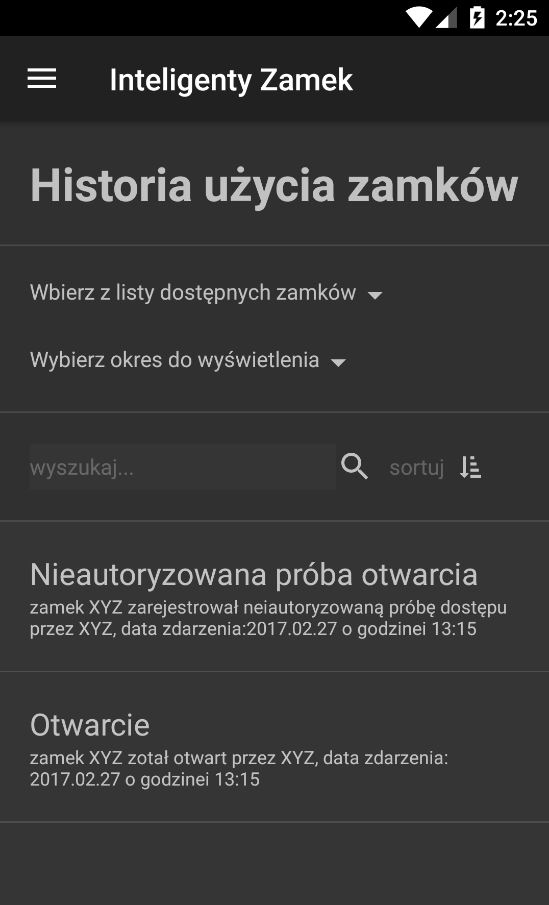
\includegraphics[width=\textwidth]{Obrazy/historia_zamkow_pionowo}
\caption{Panel historii użycia zamków (filtr)}
\label{rys:panel_historii_uzycia_zamka_pionowo}
\end{minipage}
\hspace{0.1\textwidth}
\begin{minipage}{0.45\textwidth}
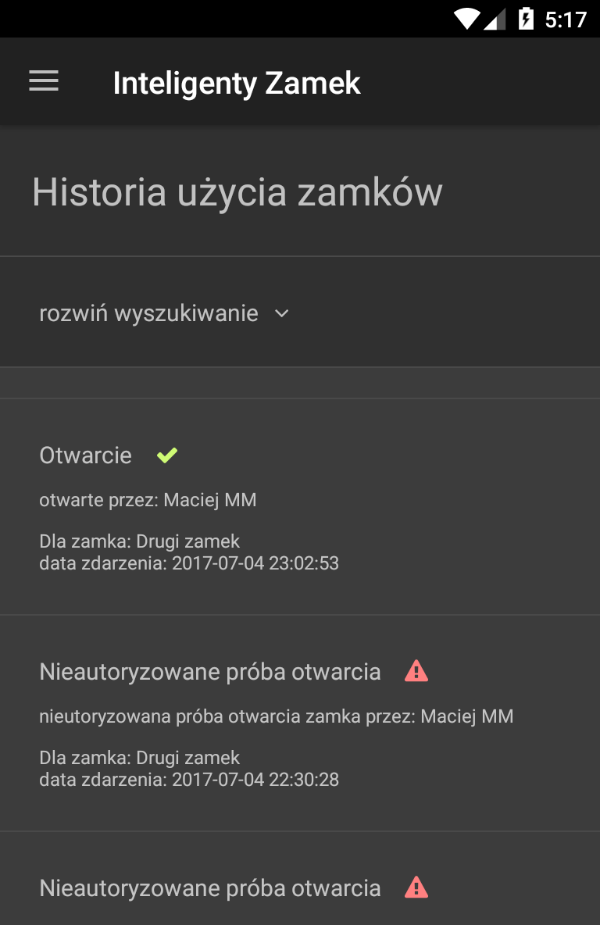
\includegraphics[width=\textwidth]{Obrazy/historia_zamkow_pionowo2}
\caption{Panel historii użycia zamków (historia)}
\label{rys:panel_historii_uzycia_zamka_pionowo2}
\end{minipage}
\end{figure}
\newpage

\paragraph*{Panel generowania nowego certyfikatu (administrator)}
Panel generowanie nowego certyfikatu (administrator) będzie służył do tworzenia nowych certyfikatów przez administratora. W pierwszych polach podaje się imię i nazwisko kogo dotyczy certyfikat.Następnie wybierane jest użytkownik (login) oraz zamek z rozwijanej listy. W dalszej części wybierane jest zakres dat w których certyfikat ma być ważny. Potem widać przycisk o nazwie ''zakres obowiązywania certyfikatów'', który przekierowuje do widoku odpowiedzialnego za to w jakich godzinach dla danych dni tygodni certyfikat udziela dostępu (Rys.~\ref{rys:panel_generowanie_nowego_klucza_gosc_admin_pioniowo}, \ref{rys:panel_generowanie_nowego_klucza_admin_pionowo2} i 
\ref{rys:panel_wyboru_zakresu_certyfikatu})

\vspace{-0.3cm}
\begin{figure}[ht!]
\begin{minipage}{0.35\textwidth}
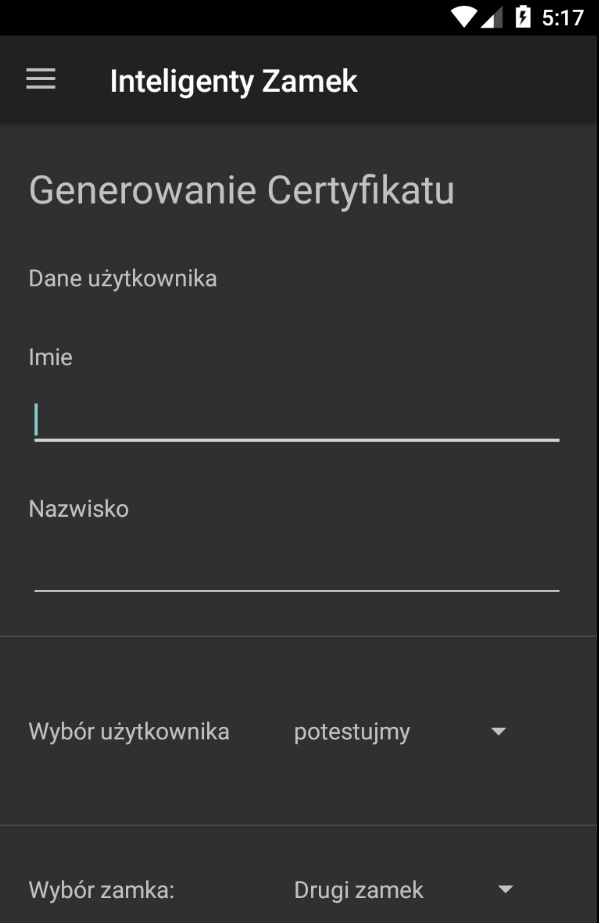
\includegraphics[width=\textwidth]{Obrazy/generowanie_nowego_klucza_gosc_admin_pioniowo}
\caption{Panel generowania nowego klucza cz. 1 }
\label{rys:panel_generowanie_nowego_klucza_gosc_admin_pioniowo}
\end{minipage}
\hspace{0.3\textwidth}
\begin{minipage}{0.35\textwidth}
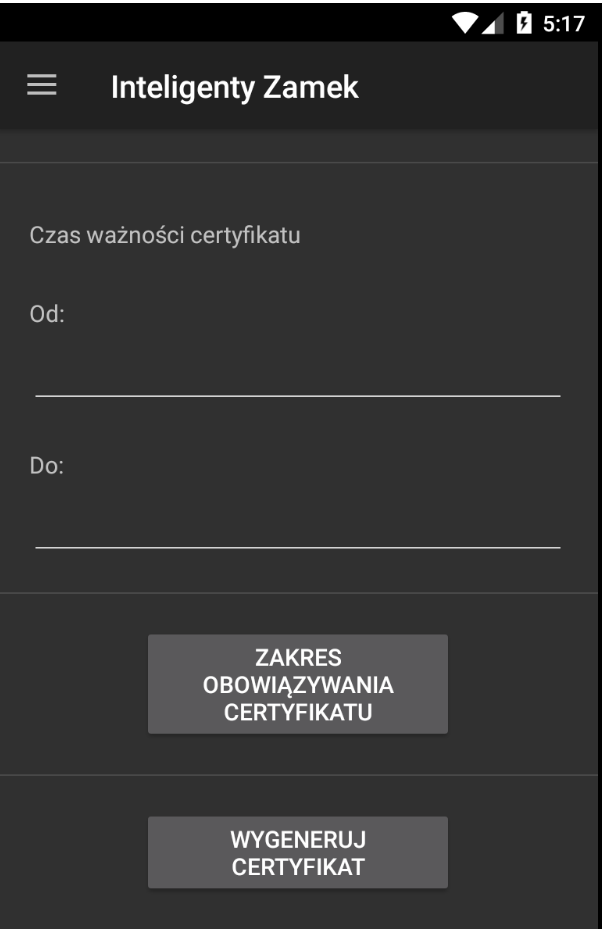
\includegraphics[width=\textwidth]{Obrazy/generowanie_nowego_klucza_admin_pionowo2}
\caption{Panel generowania nowego klucza cz. 2}
\label{rys:panel_generowanie_nowego_klucza_admin_pionowo2}
\end{minipage}
\end{figure}
\vspace{-0.55cm}
\begin{figure}[ht!]
\center
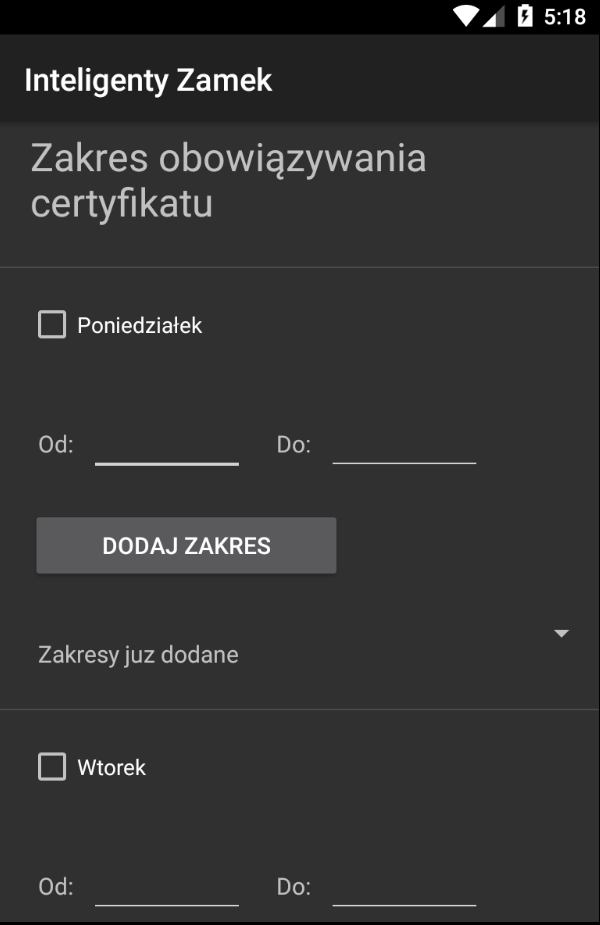
\includegraphics[width=5.8cm]{Obrazy/generowanie_nowego_klucza_uzytkownik_zalogowany_admin_pioniowo}
\caption{Panel generowania nowego klucza cz. 3}
\label{rys:panel_wyboru_zakresu_certyfikatu}
\end{figure}
\newpage

\paragraph*{Panel zarządzania certyfikatami~(administrator)}
Panel zarządzania certyfikatami użytkowników (administrator) będzie widokiem tylko wszystkich aktywnych certyfikatów w systemie. Administrator klikając na pozycję przejdzie do panelu certyfikatu opisanego wyżej. Tam może usunąć dostęp lub go przedłużyć. Ułatwieniem jest możliwość wyboru typu sortowania. (Rys. \ref{rys:panel_lista_certyfikatow_administrator_pionowo})

\begin{figure}[ht!]
\begin{minipage}{0.45\textwidth}
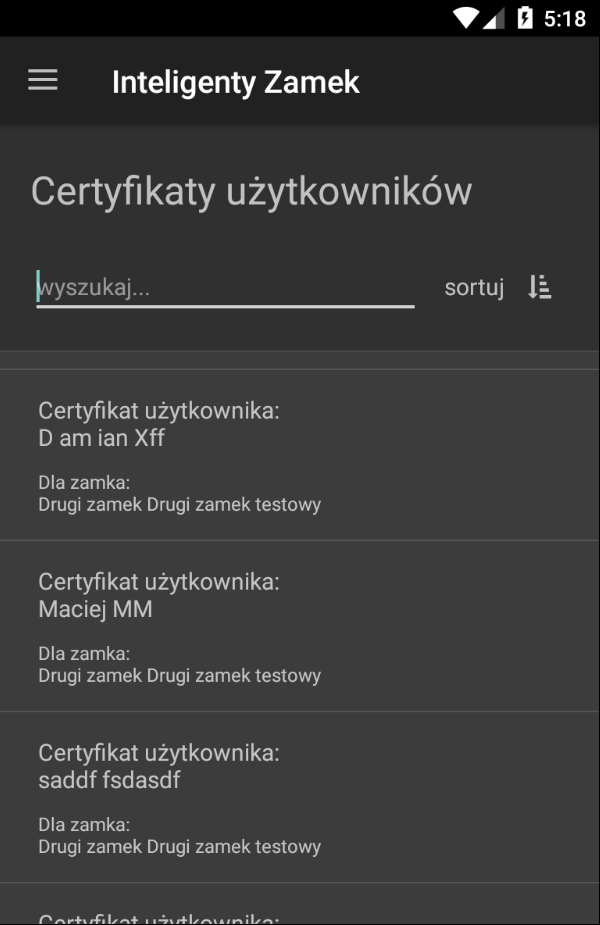
\includegraphics[width=\textwidth]{Obrazy/lista_certyfikatow_administrator_pionowo}
\caption{Panel zarządzania certyfikatami (administrator) }
\label{rys:panel_lista_certyfikatow_administrator_pionowo}
\end{minipage}
\hspace{0.1\textwidth}
\begin{minipage}{0.45\textwidth}
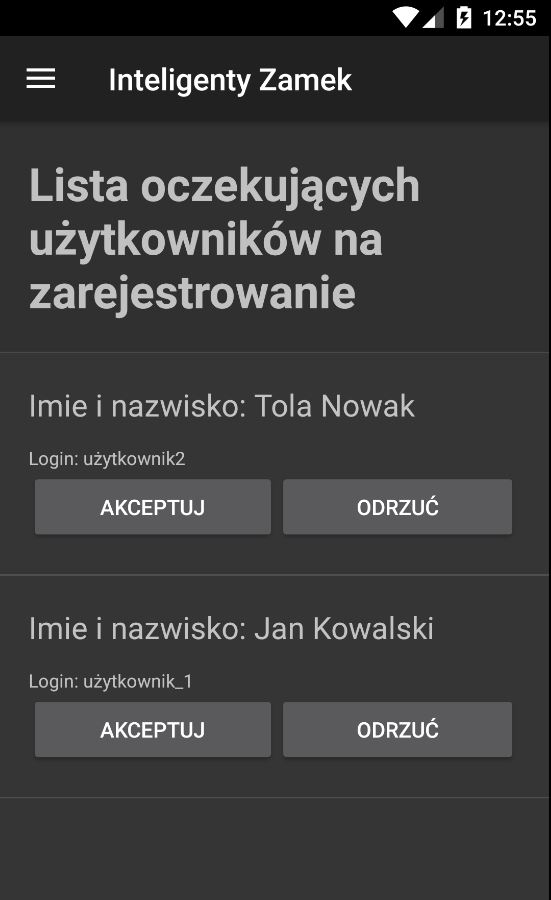
\includegraphics[width=\textwidth]{Obrazy/lista_oczekujacych_uzytkownikow_pionowo}
\caption{Panel listy oczekujących użytkowników }
\label{rys:panel_lista_oczekujacych_uzytkownikow_pionowo}
\end{minipage}
\end{figure}

\paragraph*{Panel~listy~oczekujących~użytkowników~do~rejestracji}
Panel listy oczekujących użytkowników będzie listą wszystkich gości, którzy ubiegają się o zarejestrowanie. Po kliknięciu w odpowiednią pozycję pojawiają się dwie opcję: ''AKCEPTUJ” lub ''ODRZUĆ”.  (Rys. \ref{rys:panel_lista_oczekujacych_uzytkownikow_pionowo} )
\newpage

\paragraph*{Panel~listy~oczekujących~certyfikatów do~wygenerowania}
Panel listy oczekujących certyfikatów będzie listą wszystkich certyfikatów, które ubiegającyh się o akceptację administratora. Po kliknięciu w odpowiednią pozycję pojawią się dwie opcję: ''AKCEPTUJ” lub ''ODRZUĆ”.  (Rys. \ref{rys:panel_lista_oczekujacych_certyfikatow_pionowo} )

\begin{figure}[ht!]
\begin{minipage}{0.45\textwidth}
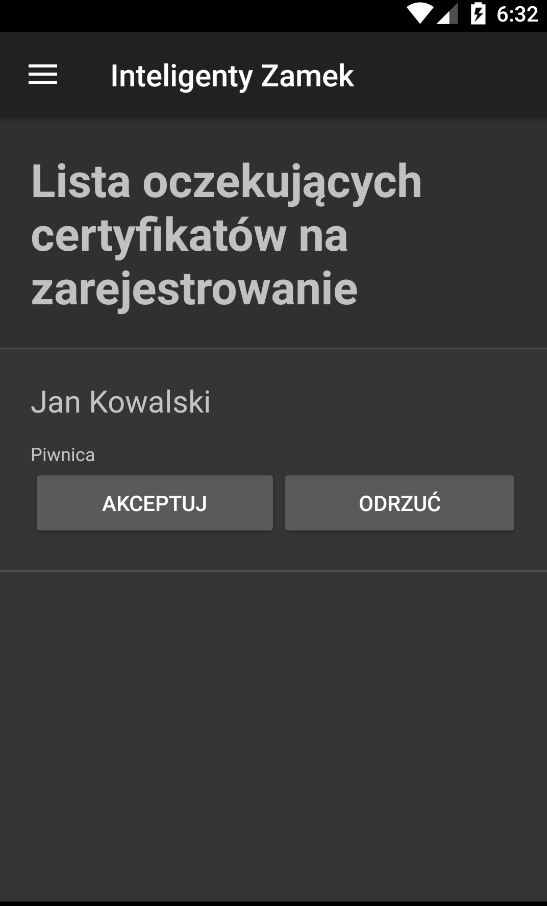
\includegraphics[width=\textwidth]{Obrazy/lista_oczekujacych_certyfikatow_pionowo}
\caption{Panel listy oczekujących certyfikatów }
\label{rys:panel_lista_oczekujacych_certyfikatow_pionowo}
\end{minipage}
\hspace{0.1\textwidth}
\begin{minipage}{0.45\textwidth}
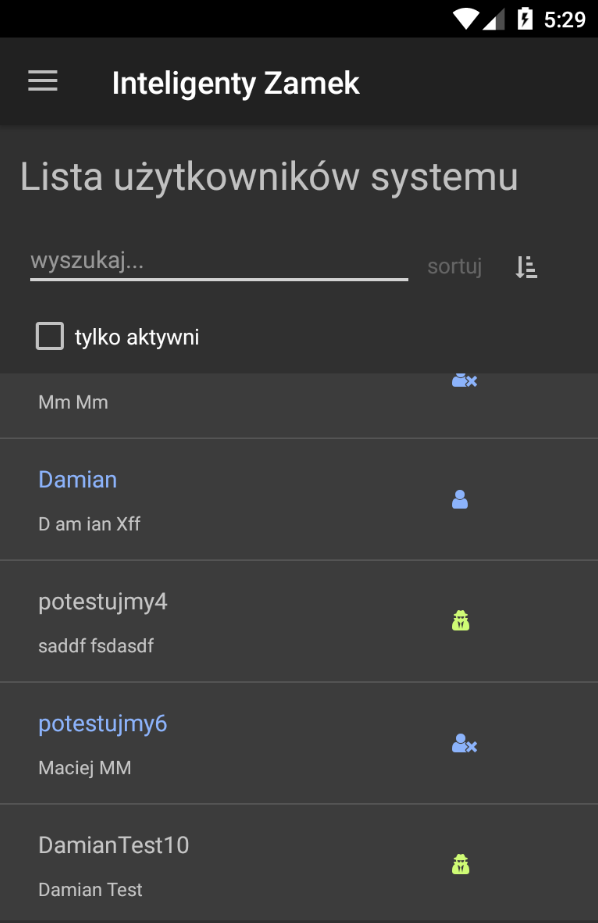
\includegraphics[width=\textwidth]{Obrazy/zarzadzanie_kontami}
\caption{Panel zarządzania kontami użytkowników}
\label{rys:panel_Zarządzania_Kontami}
\end{minipage}
\end{figure}

\paragraph*{Panel zarządzania kontami użytkowników}
Panel ten służyć będzie do zarządzania kontami użytkowników. Wyświetli on listę użytkowników systemu wraz z z oznaczeniami czy jest on aktyny bądź zablokowany oraz czy ma ważny klucz szyfrujący (Rys. \ref{rys:panel_Zarządzania_Kontami})

\newpage

\paragraph*{Panel ustawień konta}
W panelu ustawień użytkownik będzie mógł zmienić hasło do swojego konta. Wymaga podania starego hasła, a następnie nowego. Ponadto w panelu tym będzie podgląd certyfikatu szyfrującego wraz z możliwością wygenerowania nowego oraz zmianę adresu ip serwera  (Rys. \ref{rys:panel_ustawienia_pionowo} i \ref{rys:panel_ustawienia_pionowo2} i \ref{rys:panel_ustawienia_pionowo3}).

\begin{figure}[ht!]
\begin{minipage}{0.35\textwidth}
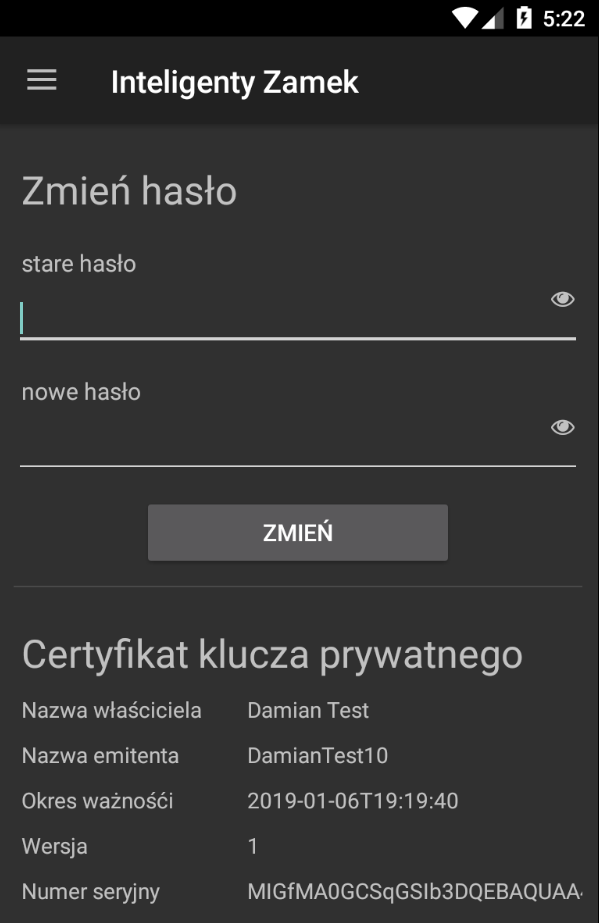
\includegraphics[width=\textwidth]{Obrazy/ustawienia_1}
\caption{Panel generowania nowego klucza cz. 1 }
\label{rys:panel_ustawienia_pionowo}
\end{minipage}
\hspace{0.3\textwidth}
\begin{minipage}{0.35\textwidth}
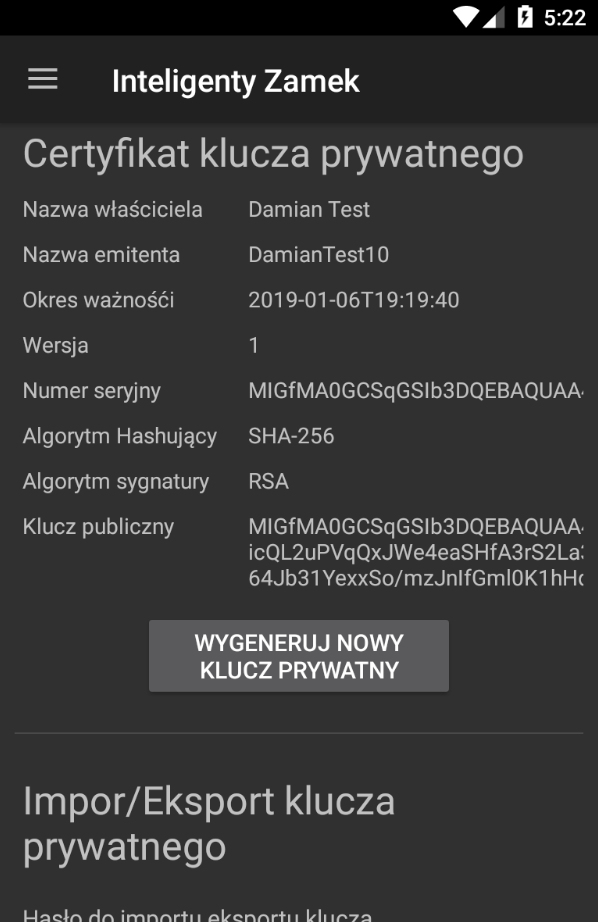
\includegraphics[width=\textwidth]{Obrazy/ustawienia_2}
\caption{Panel generowania nowego klucza cz. 2}
\label{rys:panel_ustawienia_pionowo2}
\end{minipage}
\end{figure}
\begin{figure}[ht!]
\centering
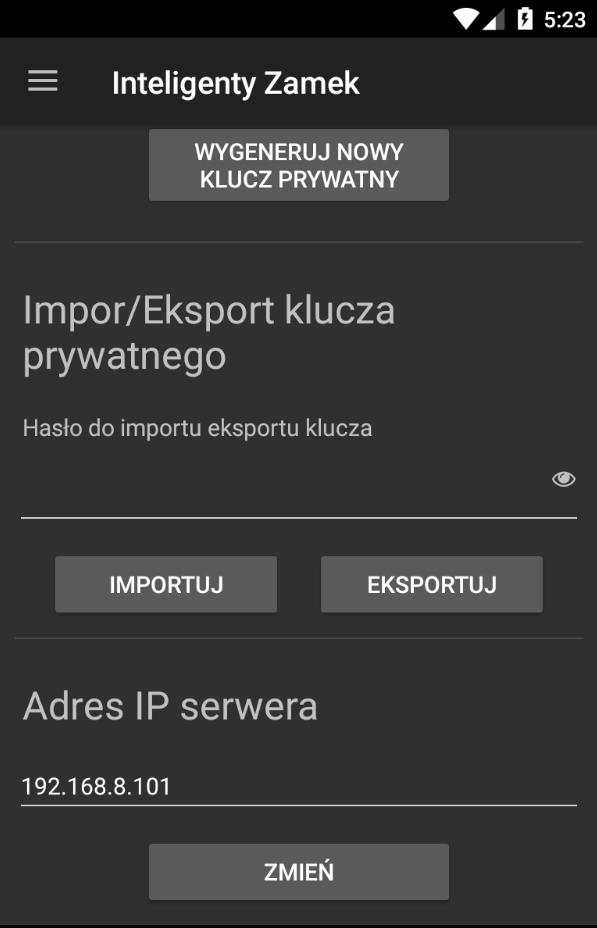
\includegraphics[width=6cm]
{Obrazy/ustawienia_3}
\caption{Panel ustawień konta (adres ip)}
\label{rys:panel_ustawienia_pionowo3}
\end{figure}
\newpage

\subsubsection{Widoki strony internetowej systemu}
Strona internetowa posiadać powinna dwa widoki, jeden widok logowania  (Rys. \ref{rys:strona_1}, w którym administrator musi wpisać login oraz hasło. W drugim widoku mamy listę historii otwarcia zamków  (Rys. \ref{rys:strona_2}) wraz z zaznaczeniem kolorystycznym które pokazuje czy była to próba autoryzowana.

\begin{figure}[ht!]
\centering
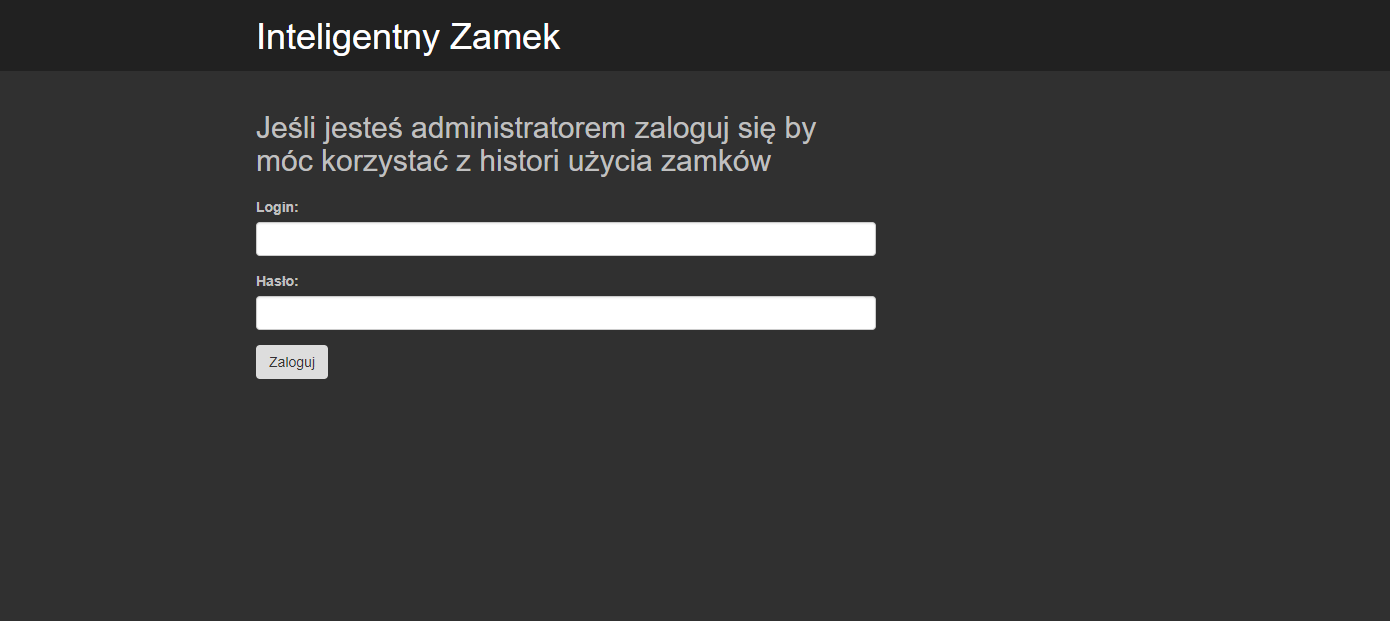
\includegraphics[width=16cm,height=10cm,keepaspectratio]
{Obrazy/strona_logowanie}
\caption{Strona logowania}
\label{rys:strona_1}
\end{figure}

\begin{figure}[ht!]
\centering
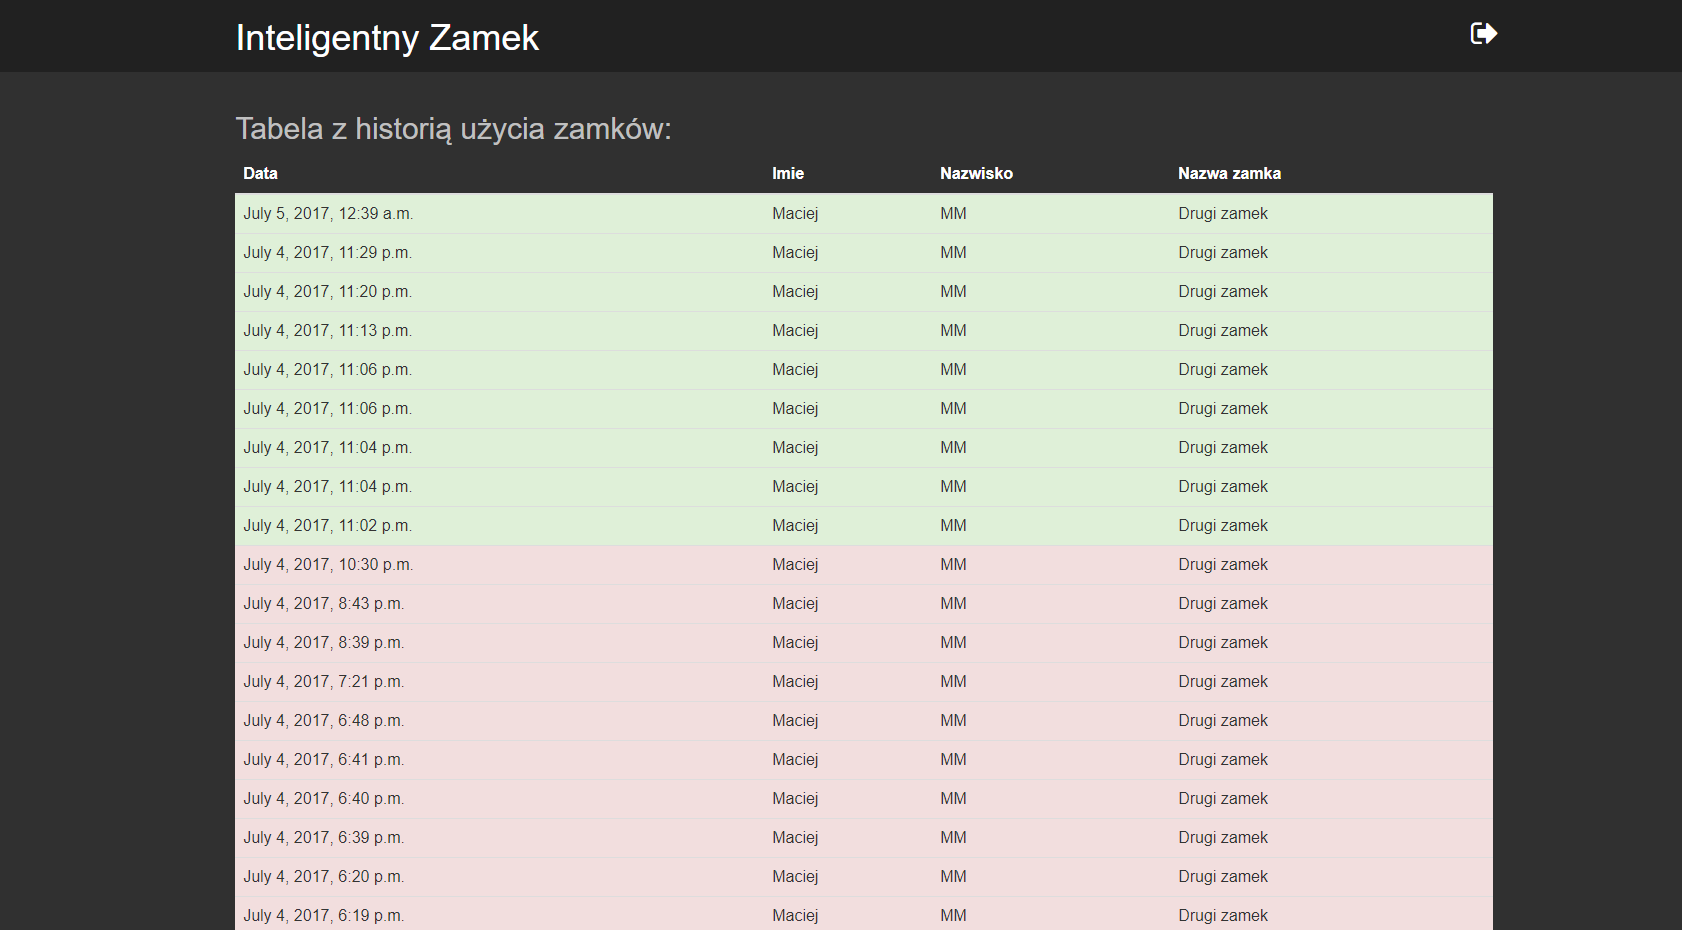
\includegraphics[width=16cm,height=10cm,keepaspectratio]
{Obrazy/strona_historia}
\caption{Strona z wyświetloną historią użycia zamków)}
\label{rys:strona_2}
\end{figure}
\newpage
\subsubsection{Komunikacja człowiek-interfejs}
Aplikacja komunikować się może z człowiekiem na wiele sposób, jednym z nich są komunikaty tekstowe lub znane symbole informujące o funkcjonalności. 
\paragraph*{Komunikaty tekstowe}
W aplikacji mobilnej komunikaty są wyświetlane przy pomocy toast. Komunikaty te  trwają na ekranie 4 sekundy. Informują one użytkownika o zaistniałych sytuacjach takich jak
\begin{itemize*}
\item błąd połączenia z bazą danych
\item informacja o zablokowanym koncie 
\item informacja o czynnościach dodania bądź usunięcia odpowiednio użytkownika bądź certyfikatu
\item o pobraniu listy certyfikatów
\end{itemize*}

Dodatkowo są wyświetlane na ekranie komunikaty tekstowe przy pomocy  textview odnośnie walidacji danych oraz podpowiedzi podczas wpisywania haseł przy pomocy tooltip-ów, które informują użytkownika o~parametrach jakie hasło powinno mieć.

\paragraph*{Symbolika ikon}\label{Symbolika ikon}
Aplikacja mobilna oraz strona internetowa korzysta z symboli zawartych w fontwesome, oto poszczególne znaczenia dla danych ikon:

\begin{longtable}[!ht]{|m{2cm}|m{10cm}|} 
\caption{Tabela ikon używanych w systemie}
\label{tab:ikony}\\
\hline
Ikona & Opis   \\ \hline


\includegraphics[width=0.6cm]{Obrazy/full_user}  &  ikona oznaczająca użytkownika  aktywnego z aktualnym kluczem szyfrującym   
\\ \hline

\includegraphics[width=0.6cm]{Obrazy/user} & ikona oznaczająca użytkownika  aktywnego z nieaktualnym kluczem szyfrującym \\ \hline

\includegraphics[width=0.6cm]{Obrazy/block_user}&ikona oznaczająca użytkownika zablokowanego \\ \hline
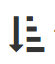
\includegraphics[width=0.6cm]{Obrazy/sort_desc}&ikonka oznaczająca sortowanie od a do z 
\\ \hline
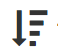
\includegraphics[width=0.6cm]{Obrazy/sort_asc}&Ikonka oznaczająca sortowanie od z do a
\\ \hline

\includegraphics[width=0.6cm]{Obrazy/oko_1} & ikonka służąca do  pokazania na ekranie hasło które było wcześniej zamaskowane
\\ \hline

\includegraphics[width=0.6cm]{Obrazy/oko_2}&Ikonka służąca do maskowania hasła
\\ \hline
\includegraphics[width=0.6cm]{Obrazy/menu}&Ikonka służąca do rozwijania menu
\\ \hline
\includegraphics[width=0.6cm]{Obrazy/menu}&Ikonka służąca do chowania menu
\\ \hline
\includegraphics[width=0.6cm]{Obrazy/lock}&Ikonka oznaczająca zamknięty zamek
\\ \hline
\includegraphics[width=0.6cm]{Obrazy/lock_2}&Ikonka oznaczająca otwarty zamek
\\ \hline
\includegraphics[width=0.6cm]{Obrazy/error}&Ikonka oznaczająca niepoprawność np. niepoprawne hasło
\\ \hline
\includegraphics[width=0.6cm]{Obrazy/ok}& oznaczająca poprawność np. poprawny dostęp do pomieszczenia
\\ \hline
\end{longtable}
\newpage
\paragraph*{Znaczenie kolorystyki}
W systemie występują 4 kolory informujące użytkownika o zaistniałych sytuacjach
\begin{itemize*}
\item czerwony który w zależności od kontekstu sugeruje albo niepoprawne wpisane dane, nie uzyskanie dostępu do pomieszczenia albo nieautoryzowaną próbę dostępu do pomieszczenia,
\item zielony który w zależności od kontekstu sugeruje poprawne uzyskanie dostępu do pomieszczeń, autoryzowaną próbę dostępu do pomieszczenia lub użytkownika który jest aktywny, lub posiada aktualny klucz szyfrujący,
\item żółty sugeruje w naszym systemie oczekiwanie na zdarzenie,
\item kolor fioletowy określa użytkownika który nie ma dostępu do funkcji systemu (w zależności od ikony ma~nieaktualny klucz szyfrujący lub ma konto zablokowane)
\end{itemize*}

\subsubsection{Kolorystyka systemu}
Kolorystyka systemu została oparta o styl material design, który jest dostępny dla systemu android od wersji 5.0. Strona jak i aplikacja mobilna są zbliżone kolorystycznie. Różnice w kolorach są spowodowane tylko narzuconą kolorystyką z biblioteki Bootsrap\cite{And,desingMobile}.

\subsection{Bezpieczeństwo systemu}\label{sec:Projekt bezpieczeństwo}
Prezentowany system ma na celu zapewniać bezpieczeństwo, zatem sam powinien być bezpieczny. Podstawowym zabezpieczeniem jakie można zastosować jest szyfrowanie połączeń oraz danych przechowywanych na nośnikach. Pierwszy sposób zapewnia wcześniej opisane w punkcie \ref{Komunikacja serwer} zastosowanie bezpiecznego protokoły Https. Druga forma zabezpieczania, mianowicie szyfrowanie odbywać się powinno głównie po stronie aplikacji mobilnej. Zdecydowano o zastosowaniu szyfrowania AES w trybie CBC, jest to wydajny algorytm, a przy tym bezpieczny (nie wykryto jak dotąd żadnych luk). Istotną kwestią bezpieczeństwa jest również weryfikacja tożsamości oraz autoryzacja w systemie.
\subsubsection{Projekt infrastruktury klucza publicznego (PKI)}\label{sec:Projekt PKI}
W pierwszej kolejności opisana zostanie przedstawiony projekt infrastruktury klucza publicznego (w skrócie PKI). Ideą infrastruktury klucza publicznego jest zarządzanie cyfrowymi certyfikatami i kluczami szyfrującymi dla osób, oprogramowania, urządzeń i systemów. Przy jednoczesnym zachowaniu integralności, poufności oraz dostępności.
\paragraph*{Certyfikat szyfrujący}
Certyfikat klucza szyfrującego ma format JSONa składającego się z następujących pól:
\begin{itemize*}
\item ''PUBLIC\_KEY” - wartość klucza publicznego pary kluczy dostępowych,
\item ''Signature\_Algorithm\_Identifier'' --- algorytm szyfrujący sygnaturę,
\item ''Validity\_period'' --- data ważności pary kluczy,
\item ''Version'' --- wersja certyfikatu,
\item ''Issuer\_name'' --- nazwa emitenta,
\item ''Hash\_Algorithm'' --- algorytm funkcji skrótu,
\item ''Serial\_number'' --- unikalna wartość dla certyfikatu,
\item ''User\_Name'' --- imię i nazwisko użytkownika.
\end{itemize*}
\newpage
Przykładowa zawartość takiego certyfikatu szyfrującego może być następująca:\\
{\footnotesize  \{\\
	''PUBLIC\_KEY'':''MIGfMA0GCSqGSIb3DQEBAQUAA4GNADCBiQKBgQC7jik\linebreak izatJoaAnSc89HJO75BRi+IUXWBOb6yfD\&nFZd5pxEmWNXxK6sKjDLfw4XbZ\linebreak sQhBDzLAQ6KvgzNx2+WUB9nBDnP00KQ1BmvOh7GWiCeXf44Xaj3\%n+k+znM7\linebreak uRW9TpTLwOZwNpJAtec89g6UC9d+1QCH3fd950zhlYxTu21DemwIDAQAB\%n'',\\
	''Signature\_Algorithm\_Identifier'':''RSA'',\\
	''Validity\_period'':''2018-12-18T20:59:29'',\\
	''Version'':1,\\
	''Issuer\_name'':''Test10'',\\
	''Hash\_Algorithm'':''SHA-256'',\\
	''Serial\_number'':''MIGfMA0GCSqGSIb3DQEBAQUAA4GNADCBiQKBgQD\linebreak gW6H2k5BeVvGbKY81X+cvnrGOKNgCN6017fKdkGceGhFAP6ZNyPxvzjhlUS\&\linebreak /ikJRsaybUiIKP\&/lxtiheEX9hdlbY19vbrCUn3CXO\&/ILXxlYANMk1eca\linebreak UTu+VWXg5\&/GEGQ4YeNJh+au78KSnYitPMJezrN8\&/t+hkTjAFt166eDJw\linebreak IDAQAB'',\\
	''User\_Name'':''Damian Test''  \\
	\}}

\paragraph*{Urzędy certyfikujące [Maciej Marciniak]}
W prezentowanym systemie urzędem certyfikującym może być aplikacja serwerowa posiadająca w bazie danych przy rekordach użytkownika w tabeli Users znajdować mogą się kolumny przechowujące certyfikaty szyfrujące. W ten sposób certyfikat zostanie przypisany do konkretnej osoby. Charakter systemu nie wymusza potrzeby przechowywania historii przypisanych certyfikatów do danego użytkownika, ponieważ w obiegu systemu nie powinna pojawić się sytuacja, gdzie będą podpisane dane starym kluczem, tak jak może się zdarzyć taka sytuacja przy podpisywaniu fizycznych dokumentów. Ze względu na brak potrzeby przechowywania certyfikatów unieważnionych, nowo wygenerowane certyfikaty mogą nadpisywać stare rekordy, skutkuje to oszczędnością pamięci systemu. 

Urzędem rejestrującym jest tylko pośrednio aplikacja serwerowa, właściwym modułem pełniącym tę funkcję jest aplikacja mobilna z uprawnieniami administracyjnymi.
\paragraph*{Klient systemu [Damian Filipowicz]}
W przypadku systemu \NazwaSys \space klientem systemu będzie Aplikacja mobilna. Będzie ona odpowiedzialna za uwierzytelnianie użytkownika w systemie oraz generowanie klucza szyfrującego, który zostanie po~tym fakcie wysyłany do urzędu certyfikującego. Sam klucz szyfrujący będzie tworzony w momencie rejestracji użytkownika oraz na żądanie użytkownika\cite{PKI}.

\subsubsection{Poufność}
Poufność zostanie zapewniona przy pomocy odpowiedniego przechowywania danych. Aplikacja będzie przechowywać newralgiczne dane systemu takie jak hasło użytkownika, jego token oraz klucz szyfrujący. Kluczową kwestią jest odpowiednie przechowywanie tych danych w telefonie tak, aby nie mógł nikt niepowołany ich uzyskać. Hasło przechowywane będzie w postaci zaszyfrowanego pliku, który będzie szyfrowany kluczem wszytym w oprogramowanie aplikacji za pomocą metody AES w trybie CBC. Token użytkownika oraz klucz szyfrujący będzie przechowywany jako plik w smartphonie i szyfrowany hasłem użytkownika. Dzięki temu nawet jeżeli niepowołana osoba uzyska dostęp do danych plików nie będzie w stanie ich odszyfrować w łatwy sposób.

Drugim newralgicznym punktem aplikacji mobilnej będzie transmisja danych, dlatego w komunikacji pomiędzy serwerem, a urządzeniem mobilnym wykorzystany będzie protokół Https. Co uniemożliwi podsłuch danych. Pomiędzy uprzędzeniem sterującym, a telefonem komunikacja poprzez bluetooth zabezpieczona jest kluczem aplikacji. Mechanizm ten powoduje, że żadna aplikacja nie posiadająca danego kodu nie będzie w stanie połączyć się z aplikacjami prezentowanego systemu.

\subsubsection{Dostępność}
Dzięki popularności aplikacji mobilnych prezentowany system będzie w dużym stopniu dostępny dla użytkowników. Jedynymi zagrożeniami będzie awaria sieci komputerowej, w której znajdować będzie się serwer oraz awaria sieci elektrycznej. Pierwsze jak i drugie zagrożenie będziemy redukować w postaci możliwość uzyskania dostępu do pomieszczeń w tradycyjny sposób przy pomocy kluczy (przy zastosowaniu rozwiązania z elektrozamkiem, które nie wymaga ingerencji w mechanizm oryginalny). Ponadto drugie zagrożenie będzie też redukowane przy pomocy urządzeni awaryjnego zasilania, co umożliwi funkcjonowanie systemu po zaniku napięcia w sieci elektrycznej przez określony czas.
\subsubsection{Integralność}
Integralność zasobów zapewniona jest dzięki pośredniczeniu aplikacji serwerowej w dostępie do bazy danych. Modyfikacje w bazie danych wprowadzić można tylko pośrednicząc przez serwer, który weryfikuje uprawnienia i filtruje możliwe odwołania do informacji, do których nie posiada użytkownik dostępu. Wprowadzać modyfikacje będzie mógł ewentualnie administrator po wcześniejszym zalogowaniu się do aplikacji zarządzającej bazą danych.

\newpage\section{Implementacja} \label{sec:implementacja}
Rozdział przedstawia opis wybranych technik użytych do utworzenia głównych funkcji systemu. Techniki te zostały podzielone na cztery kategorie:
\begin{itemize*}
\item Aplikacja mobilna opisująca implementacje przechowywania danych, graficznych widoków, walidacji danych oraz komunikacji z serwerem. 
\item Serwer opisujący implementację serwera  oraz strony internetowej wraz z opisem komunikacji między oprogramowaniem serwera a bazą danych.
\item  Urządzenie sterujące opisujące implementację urządzenia odpowiedzialnego za sterowanie fizyczne dostępem do zamka wraz z komunikacją z serwerem.
\item Moduł zliczania osób opisujące oprogramowanie odpowiedzialne za zliczanie osób w danym pomieszczeniu. 
\end{itemize*} 
\subsection[Aplikacja mobilna]{Aplikacja mobilna [\StudentB]}
Aplikacja mobilna jest  modułem odpowiedzialnym za interakcję użytkownika z systemem. Umożliwia on autoryzację, zarządzanie przez administratora systemem oraz uzyskiwanie dostępu do pomieszczenia.
\subsubsection{Przechowywanie danych}
W aplikacji mobilnej zostały zaimplementowane 3 możliwości przechowywania danych. Pierwszą z nich jest możliwość trzymania ich w pamięci telefonu jako pliki. Obiekty te przechowywane są w katalogu aplikacji. Przechowują one odpowiednio:
\begin{itemize*}
\item klucz szyfrujący użytkownika zaszyfrowany hasłem użytkownika
\item certyfikat klucza szyfrującego 
\item certyfikaty dostępowe
\end{itemize*}

Istnieje możliwość eksportowania dwóch pierwszych plików (Listing: \ref{lst:kod1}) ze względu na brak możliwości ich odzyskania oraz umożliwieni użytkownikowi z korzystania w wielu urządzeniach z tego samego klucza szyfrującego. W przypadku kiedy użytkownik zgubi telefon lub  wyczyści dane aplikacji to wszystkie dane znajdujące się w pamięci telefonu zostaną skasowane. Eksport ten odbywa się w widoku ustawień. Te dwa pliki zostają połączone w jeden plik który zostaje zaszyfrowany hasłem. Plik zapisywany jest w miejscu na telefonie gdzie wskażę użytkownik.  Operacje na pliku wykonywane są przy pomocy klasy statycznej ''FileReadWriteApi''.

Wybór  tej technologi do wymienionych powyższych danych jest uzasadniony zwiększoną trwałością ich w stosunku do danych przechowywanych w pamięci aplikacji jak np.  w klasie globalnej oraz możliwość przechowywania bardziej skomplikowanych danych.

Drugim sposobem przechowywania danych jest funkcja androidowa SharedPreferences. Przechowuje ona proste typy danych takiej jak int, string, char, bool w postaci klucz (wartość typu string) value (wartość z danego typu, który się podało). W pamięci tej przechowuje takie dane jak:
\begin{itemize*}
\item adres ip serwera,
\item login użytkownika,
\item hasło użytkownika zaszyfrowane kluczem wszytym w oprogramowanie,
\item token sesji użytkownika,
\item informacja czy użytkownik aplikacji jest zalogowany,
\item informacja czy użytkownik aplikacji jest administratorem.
\end{itemize*}
\newpage
\begin{lstlisting}[caption={Funkcja eksportująca klucz szyfrujący.}, label={lst:kod1}, language=Kotlin]
fun exportKey(path:String,password:String){
  if(!Valdiation.isCorrectPassword(password)){
    view.showMessage("niepoprawne haslo")
    view.showErrorPasswordKey()
  }
  try {
    val privateKey = fileReadWriteApi.readFromFile("*" + model.login, view)
    val publicCert = fileReadWriteApi.readFromFile("**" + sharedPreferenceApi.getString(view, EnumChoice.login), view)
    val str = "{\"public\":" + publicCert + ", \"private\": \"" + privateKey + "\"}"
    val toSend = CyptographyApi.encrypt(str, password)
    fileReadWriteApi.writeToFile(toSend, view, path, true)
    view.showMessage("poprawnie wyeksporotwano certyfikat")
  }
  catch (ex:Exception){
    view.showMessage("Wystapil blad podczas eksportu pliku")
  }
}
\end{lstlisting}

Ponadto przechowuje informacje wykorzystywane w widokach generowania certyfikatu takie jak:
\begin{itemize*}
\item wybór loginu,
\item wybór zamka,
\item imię, 
\item nazwisko.
\end{itemize*}

Przykładowy fragment kodu odczytujący dane z SharedPreferences znajduje się na Listingu \ref{lst:kod2}. Dzięki temu rozwiązaniu unikamy ''literówek'', które powodować, by mogły błędy w odczycie danych. 

\begin{lstlisting}[caption={Fragment kodu odpowiedzialny za odczytanie tokenu}, label={lst:kod2}, language=Kotlin]
val token = CyptographyApi.decrypt( sharedPreferenceApi.getString (view, EnumChoice.token))
\end{lstlisting}

Wybór tej technologi został podyktowany zwiększona trwałością danych w stosunku do klasy globalnej oraz prostotą w użytkowaniu jej. Żeby jeszcze bardziej ułatwić wykorzystywanie tej techniki została napisana specjalna klasa statyczna SharedPreferencesApi, w której został zaimplementowany klasa EnumChoice \linebreak (Listing \ref{lst:kod3}) przechowujący wszystkie klucze.

\begin{lstlisting}[caption={klasa EnumChoice.}, label={lst:kod3}, language=Kotlin]
enum class EnumChoice(val value:String){
  ip("ipserwer"),
  password("password"),
  token("sessionToken"),
  login("login"), 
  nameuser("name"), 
  surname("surname"),
  isLogin("isLogin"), 
  isAdmin("isadmin"),
  choiceLogin("choiceLogin"), 
  choiceLock("choiceLock"),
  publicKey("publicKey")
}
\end{lstlisting}

Trzecim sposobem jest przechowywanie w klasie globalnej (GlobalContainer)  obiektów. Przechowywane w niej są wszystkie dane które nie wymagają przechowywania po wyłączeniu aplikacji.

\subsubsection{Implementacja graficzna}

Wszystkie wartości typu string wyświetlane na ekranie są przechowywane w pliku Strings znajdującego się w katalogu res/values. Wybór takiego sposobu został podyktowany faktem możliwości późniejszego łatwiejszego przerabiania tekstów oraz możliwości łatwiejszego tłumaczenia na inny język. Wszystkie kolory użyte w aplikacji przechowywane są w pliku colors. Ma to na celu ułatwienie  zmiany kolorów w całej aplikacji. Styl dla podstawowych elementów graficznych takich jak ''editText'', ''TextView'' czy ''Button'' przechowywane są w pliku styles co ma za zadanie umożliwienie łatwiejszej zmiany wyglądów danych elementów w całej aplikacji.

Oprócz stylów elementów, czy wartości tekstowych należy również napisać, w jaki sposób generowane są widoki. Widoki te są przechowywane w plikach XML.  Dla widoków które nie posiadały listy został zaimplementowany układ ''LinearLayout'' ze względu na prostotę w tworzeniu oraz ewentualnych zmianach w wyglądzie. Natomiast dla widoków z wyświetlanymi jakimiś listami został zaimplementowany układ ''ConstrainLayout'' ze względu na fakt że przy liście występuje znacznie więcej odwołań do generowania widoku a układ ten jest pod tym względem o wiele wydajniejszy od wspomnianego wcześniej ''LinearLayout''\cite{desingMobile}.

\subsubsection{Walidacja danych wprowadzanych przez użytkownika}
Walidacja danych wprowadzonych przez użytkownika odbywa Się przy pomocy klasy statycznej Validation. Klasa ta udostępnia cztery funkcje odpowiedzialne za:
\begin{itemize*}
\item poprawność formatu adresu ip ,
\item czy data podana w drugim parametrze jest datą późniejszą niż data podana w pierwszym parametrze (Listing \ref{lst:kod5}),
\item poprawność hasła,
\item poprawność loginu.
\end{itemize*}

Wyrażenia regularne użyte w tych funkcjach znajdują się na Listingu \ref{lst:kod4}.

\begin{lstlisting}[caption={Wyrażenia regularne.}, label={lst:kod4}, language=Kotlin]
"^(?=.*[0-9])(?=.*[A-Z])(?=.*[@#$%^&+=!])(?=\\S+$).{4,}$"

"^((0|1\\d?\\d?|2[0-4]?\\d?|25[0-5]?|[3-9]\\d?)\\.)
{3}(0|1\\d?\\d?|2[0-4]?\\d?|25[0-5]?|[3-9]\\d?)$"
\end{lstlisting}

\begin{lstlisting}[caption={Funkcja odpowiedzialna za sprawdzanie, która data jest pó"zniejsza.}, label={lst:kod5}, language=Java]
public static boolean biggerThanTime(String time1,String time2){
  Date date = new Date() ;
  SimpleDateFormat dateFormat = new 
  SimpleDateFormat("HH:mm") ;
  dateFormat.format(date);
  try 
  {
    if (dateFormat.parse(time1).after( dateFormat.parse(time2))) {
      return false;
    } else {
      return true;
    }
  }
  catch (Exception ex){}
  return false;
}
\end{lstlisting}

\subsubsection{Komunikacja z serwerem}
Do komunikacji z serwerem napisana została specjalna klasa dziedzicząca po klasie AsyncTask o nazwie HTTPRequest. Klasa ta wysyła podane w konstruktorze (listing \ref{lst:kod6}) w postaci Hashmap-u dane do serwera i~po~otrzymaniu informacji zwrotnej z serwera przekazuje tą odpowiedź. Odpowiedź ta jest przekazywana do~klasy która utworzyła i wykonała klasę HTTPRequests do funkcji o nazwie podanej w parametrze konstruktora przy pomocy refleksji (listing: \ref{lst:kod7}). Dzięki temu klasa ta jest uniwersalna i Może być stosowana w każdym miejscu programu.

\begin{lstlisting}[caption={Konstruktor klasy HTTPRequest.}, label={lst:kod6}, language=Java]
public HTTPRequestAPI(Object presenter,String url,String methodName,HashMap DataToSend) {
  this.urlString=url;
  this.DataToSend=DataToSend;
  this.methodName=methodName;
  this.presenter=presenter;
}
\end{lstlisting}

\begin{lstlisting}[caption={Metoda OnPost zwracająca odpowied"z serwera.}, label={lst:kod7}, language=Java]
@Override
protected void onPostExecute(String response) {
  java.lang.reflect.Method method;
  try {
    method = presenter.getClass().getMethod(methodName, String.class);
    method.invoke(presenter, response);
  }
  catch(Exception ex){}
}
\end{lstlisting}

\subsection{Serwer}
Serwer systemu zarządza wszystkimi informacjami, jest pośrednikiem w przekazywaniu i modyfikacji rekordów z bazy danych MySQL. Emulowaniem środowiska MySQL oraz Apache zajmuje się program XAMP w~wersji 3.2.2.

\subsubsection{Aplikacja serwerowa [\StudentA]}\label{sec:apk serw}
Aplikacja serwerowa została zaimplementowana przy użyciu języka programowania Python 2.7 oraz frameworku Django. Program  właściwie składa się głównie z 3 plików:
\begin{itemize*}
\item setting.py --- odpowiedzialny za konfigurację połączenia z bazą danych, zwracanymi komunikatami, kodowanie, strefą czasową i innymi parametrami o mniejszym znaczeniu,
\item urls.py --- przechowywana tu tablica obiektów URL ustala, dla jakiego adresu URL (pierwszy parametr), wykonać konkretną metodę (parametr view), listing \ref{lst:python url} przedstawia fragment pliku urls.py,
\item views.py --- główny skrypt serwera, zawiera główną logikę aplikacji, to znaczy metody wykonywane dla konkretnych adresów URL.
\end{itemize*}

{\footnotesize 
\begin{lstlisting}[caption={Fragment pliku urls.py}, label={lst:python url}, language=Python]
urlpatterns = [
  url(r'^$', views.website, name='home'),
  url(r'^login/$', auth_views.login, {'template_name': 'login.html'}, name='login'),
  url(r'^logout/$', auth_views.logout, {'template_name': 'logged_out.html'}, name='logout'),
  url(r'^list/$', views.website, name='list'),
  url(r'^api/login/$', views.api_login, name='api_login'),
  ...
]
\end{lstlisting}}

Funkcjonalności systemu w  dużej mierze wymagają stanu zalogowania, weryfikowane jest to przez podanie od użytkownika loginu oraz tokenu sesji logowania. Pola uzyskane w zapytaniu Http w metodzie POST są~porównywane z znajdującymi się w bazie danych. Przykładowe API wymagające weryfikacji logowania znajduje się w listingu \ref{lst:serwer weryfikacja}. Użytkownik wysyła pole ''login'' oraz ''token'', następnie wykonane zostaje zapytanie do bazy danych o aktualnie znajdującą się wartość w rekordzie. Jeżeli wartości się pokrywają i nie są puste, może zostać wykonane polecenie, które chciał wywołać użytkownik. Dodatkowo, gdy operacja wymaga uprawnień administratora, weryfikowana jest flaga w bazie danych, czy dany użytkownik jest administratorem (IS\_ADMIN). Wiersze try except służą nie tylko do zamaskowania błędów działania aplikacji, ale również do zabezpieczenia programu przed podatnością SQL Injection (eliminacja tak zwanego feed backu o błędach przy próbie podawania innych wartości niż zaplanowano w systemie).

Operacje logowania i rejestracji są podstawowymi działaniami, dzięki którym będzie można wykonywać bardziej złożone działania oraz niezbędne do poprawnego funkcjonowania PKI. Listing \ref{lst:serwer login} i listing \ref{lst:serwer register} przedstawiają kompletne funkcje logowania i rejestracji użytkowników. 

{\footnotesize 
\begin{lstlisting}[caption={Przykładowe API weryfikujące stan logowania}, label={lst:serwer weryfikacja}, language=Python]
def api_download_all_locks(request):
  if request.method == 'POST':
    login = request.POST.get('login')
    token = request.POST.get('token')
    try:
      cursor = db.cursor()
      cursor.execute("SELECT TOKEN FROM USERS WHERE login='%s'" % login)
      token_from_DB = cursor.fetchone()[0]
      if (token_from_DB == token and token != None):
        ...
    except Exception:
      return JsonResponse({"status": "Invalid"})
\end{lstlisting}}

Logowanie wymaga podania loginu w polu 'username' oraz skrótu SHA-256 hasła użytkownika. W pierwszej kolejności (linia 5 do 9) tworzony jest ciąg pseudolosowy, który będzie użyty jako token sesji logowania. Zastosowany generator jest wbudowany w bibliotekę RSA, w tym wypadku tworzone ciągi są kluczem publicznym algorytmu RSA. Następnym krokiem jest pobranie skrótu hasła oraz flag (czy jest administratorem, status konta) z bazy danych. Wiersz 15 decyduje, czy konto użytkownika jest aktywne, jeśli nie, to w linii 24 sprawdzane jest, czy konto zostało aktywowane, jeśli tak, oznacza to, że dane konto zostało zablokowane. W przypadku jednak, gdy konto ma status aktywny, następuje aktualizacja wartości tokenu w bazie danych oraz weryfikacja uprawnień użytkownika. Zwrócony status logowania jako root oznacza, zalogowanie się jako administrator.

Operacja rejestracji wymaga podania unikalnego dla systemu loginu, hasła w postaci skrótu SHA-256, imienia, nazwiska użytkownika oraz wygenerowany klucz publiczny RSA. Pierwszym etapem rejestracji jest weryfikacja, czy podany login znajduje się obecnie w bazie danych użytkowników. W tym celu wykonywane jest zapytanie SQL z filtrem podanego loginu, w przypadku, gdy polecenie zwróci pustą wartość (w języku Python None), oznacza to brak istnienia danego użytkownika w bazie. W przeciwnym wypadku, otrzymania wartości z zapytania, zostaje zwrócona przez serwer odpowiedź błędu loginu (ERROR~LOGIN).

Wiersze 15 do 22 skryptu \ref{lst:serwer register} tworzą certyfikat szyfrujący. Pierwszych 5 linii generuje pseudolosową wartość (wg algorytmu RSA dla klucza publicznego), będącą unikalnym identyfikatorem dla certyfikatu szyfrującego. Następnie dodawany do bazy danych jest użytkownik wraz z utworzonym certyfikatem z polami odpowiednio Public\_Key (przesłany klucz publiczny od użytkownika), Serial\_number (wygenerowana wartość pseudolosowa) oraz Validity\_period (obecna data przedłużona o rok), pozostałe wartości są domyślne (klucz szyfrujący RSA, funkcja skrótu SHA-256 i wersja certyfikatu 1).

Wiersze od 23 do końca funkcji pobierana jest kompletna zawartość certyfikatu (w formacie JSON), która następnie przesyłana jest, jako odpowiedź zwrotna dla użytkownika. W przypadku błędu konwersji rekordu z bazy danych na format JSON lub błędu bazy danych zwrócona zostanie informacja o błędnym wykonaniu polecenia (status invalid w sytuacji braku dodania certyfikatu do bazy danych lub status ERROR, gdy pojawi się nieokreślony błąd podczas wykonywania procesu rejestracji)\cite{programowanie_aplikacji_webowych}.
\newpage

{\footnotesize
\begin{lstlisting}[caption={API rejestracji}, label={lst:serwer register}, language=Python]
def api_register(request):
  if request.method == 'POST':
    login = request.POST.get('login')
    password = request.POST.get('password')
    name = request.POST.get('name')
    surname = request.POST.get('surname')
    publickkey = request.POST.get('publickkey')
    
    cursor = db.cursor()
    cursor.execute("SELECT LOGIN FROM USERS WHERE LOGIN='%s'" % login)
    data = cursor.fetchone()
    
    if data is not None:
      return JsonResponse({"status": "ERROR LOGIN"})
    else:
      try:
        random_generator = Random.new().read
        key = RSA.generate(1024, random_generator).publickey().exportKey()
        serial = ""
        for x in key.split("\n")[1:-1]:
          serial += x
        record = [login, password, name, surname, '0', publickkey, '1', serial, datetime.now().replace(year=datetime.now().year + 1)]
        cursor.execute( 'INSERT INTO USERS (LOGIN,PASSWORD,NAME,SURNAME,IS_ADMIN,PUBLIC_KEY, ISACTIVATED, Serial_number, Validitiy_period) VALUES(%s,%s,%s,%s,%s,%s,%s,%s,%s)', record)
        db.commit()
        cursor.execute( "SELECT CONCAT(NAME, ' ', SURNAME) as User_Name, LOGIN as Issuer_name,  PUBLIC_KEY, Serial_number, Validitiy_period, Version, Signature_Algorithm_Identifier, Hash_Algorithm FROM `users` WHERE `LOGIN` = '%s'" % (login))
        db.commit()
        dict_certificate = [dict((cursor.description[i][0], value) for i, value in enumerate(row)) for row in cursor.fetchall()]
        if len(dict_certificate) == 0:
          return JsonResponse({"status": "invalid"})
        else:
          return JsonResponse({"status": "ok", "data": dict_certificate})
      except Exception:
        db.rollback()
        return JsonResponse({"status": "ERROR"})
\end{lstlisting}}
\newpage
{\footnotesize 
\begin{lstlisting}[caption={API logowania}, label={lst:serwer login}, language=Python]
def api_login(request):
  if request.method == 'POST':
    username = request.POST.get('username')
    password = request.POST.get('password')
    
    random_generator = Random.new().read
    key = RSA.generate(1024, random_generator).publickey().exportKey()
    token = ""
    for x in key.split("\n")[1:-1]:
      token += x
    
    try:
      cursor = db.cursor()
      cursor.execute("SELECT PASSWORD, IS_ADMIN, ISACTIVATED FROM USERS WHERE login='%s'" % username)
      data = cursor.fetchone()
      if data[2] == 0:
        if data[0] == password:
          cursor.execute("UPDATE USERS SET TOKEN = '%s' WHERE LOGIN = '%s'" % (token, username))
          db.commit()
          if data[1] == 1:
            return JsonResponse({"status": "root", "token": token})
          else:
            return JsonResponse({"status": "ok", "token": token})
        else:
          return JsonResponse({"status": "ERROR PASSWORD", "token": "invalid"})
      elif data[2] == 1:
        return JsonResponse({"status": "not activated", "token": "invalid"})
      else:
        return JsonResponse({"status": "blocked", "token": "invalid"})
    except Exception:
      return JsonResponse({"status": "ERROR", "token": "Invalid"})
\end{lstlisting}}

\subsubsection{Strona internetowa [\StudentB]}
Strona internetowa została dopisana do projektu serwera w oparciu o framework Django. Zaimplementowane są trzy widoki. Widok logowania, widok wyświetlający historię oraz widok do którego przechodzi się po wylogowaniu. Główny widok możliwy jest do wyświetlenia tylko po zalogowaniu. Login oraz hasło używane do zalogowania należy wygenerować podczas konfiguracji serwera przy pomocy polecenia ''python manage.py createsuperuser'' lub modyfikując wpis w bazie danych ręcznie. Strona internetowa znajduje się w plikach:
\begin{itemize*}
\item views.py
\item urls.py
\item *.html
\end{itemize*}

W pliku ''urls.py''(Listing: \ref{lst:python url}) znajdują się adresy URL które korzystają z wbudowanej funkcji django ''auth\_views.login'' służącej do logowania oraz ''auth\_views.logout'' służąca do wylogowania. Plik ''views.py'' posiada API (Listing: \ref{lst:serwer login strona}) wykorzystywane w stronie głównej które pobiera z bazy danych. W plikach z rozszerzeniem html znajduje się implementacja wyglądu strony.

{\footnotesize 
\begin{lstlisting}[caption={API logowania do strony internetowej}, label={lst:serwer login strona}, language=Python]
@login_required(login_url="login/")
def website(request):
  try:
    cursor = db.cursor()
    cursor.execute("SELECT DATE, ACCESS, locks_keys.NAME, locks_keys.SURNAME, locks.NAME AS 'ZAMEK' FROM access_to_locks, locks_keys, locks WHERE locks_keys.ID_KEY = access_to_locks.ID_KEY AND locks.ID_LOCK = access_to_locks.ID_KEY ORDER BY DATE DESC")
    rows = cursor.fetchall()
  finally:
    return render_to_response('home.html', {"rows": rows})
\end{lstlisting}}
\subsection{Urządzenie sterujące [\StudentA]}
Program urządzenia sterującego nasłuchuje połączeń bluetooth (jest serwerem) od urządzeń mobilnych. Aplikacje korzystają z bezpiecznego trybu komunikacji, to znaczy posiadają wbudowany klucz, który musi być po obu stronach połączenia identyczny. Fragment kodu odpowiedzialny za utworzenie bezpiecznego serwera znajduje się w Listingu \ref{lst:RPI bt}. Wiersz związany z kluczem aplikacji znajduje się w linii 5, w linii 6 zostaje przypisany do usług serwera. Każde nawiązanie połączenie z urządzeniem sterującym zostaje odnotowane w pliku log, tak samo jest z odebranymi danymi oraz decyzją przyznania dostępu.

{\footnotesize 
\begin{lstlisting}[caption={Tworzenie serwera bluetooth}, label={lst:RPI bt}, language=Python]
  server_sock = BluetoothSocket(RFCOMM)
  server_sock.bind(("", PORT_ANY))
  server_sock.listen(1)
  port = server_sock.getsockname()[1]
  uuid = "fa87c0d0-afac-11de-8a39-0800200c9a66"
  advertise_service(server_sock, "BluetoothChatSecure", service_id=uuid, service_classes=[uuid, SERIAL_PORT_CLASS], profiles=[SERIAL_PORT_PROFILE])
\end{lstlisting}}
Istotną rolą urządzenia sterującego jest weryfikacja poprawności certyfikatów. Sprawdzając klucze dostępowe ważne jest potwierdzenie, czy dany klucz ma przyznane uprawniania w konkretnym przedziale czasowym, odpowiedzialna za to jest funkcja ''Check\_access'' znajdująca się w Listingu \ref{lst:RPI check access}. Objaśnienie umieszczonego kodu:
\begin{itemize*}
\item wiersz 2 --- weryfikacja, czy certyfikat jest aktualny (''None'' oznacza stan aktywny),
\item wiersz 3 --- sprawdzenie ważności certyfikatu, czy obecna data mieści się pomiędzy datą od której jest ważny certyfikat (date\_from) oraz datą do której jest ważny (date\_to),
\item  wiersz 4 --- sprawdza specjalną flagę ważnego certyfikatu, czy posiadany jest dostęp stały, bez ograniczania godzin w poszczególnych dniach,
\item wiersze 6 do 21 --- analiza godzin, w których certyfikat ma dostęp, gdy nie jest ustawiona flaga dostępu stałego,
\item w każdym niespełnionym wyżej opisanym przypadku zostanie odrzucony dostęp.
\end{itemize*}

{\footnotesize 
\begin{lstlisting}[caption={Funkcja Check-access urządzenia sterującego}, label={lst:RPI check access}, language=Python]
def Check_access(certificate):
  if certificate.isactual is None:
    if datetime.strptime(certificate.date_from, '%Y-%m-%dT%H:%M:%S') < datetime.now() < datetime.strptime( certificate.date_to, '%Y-%m-%dT%H:%M:%S'):
      if certificate.ispernament == 1:
        return True
      else:
        try:
          day_access = certificate.access_table[date.today().weekday()].split(";")
        except Exception:
          day_access = []
        now = datetime.now()
        if len(day_access) > 0:
        for x in day_access:
          x = x.split("-")
          try:
            x0 = x[0].split(":")
            x1 = x[1].split(":")
            if datetime.now().replace(hour=int(x0[0]), minute=int(x0[1])) <= now < datetime.now().replace(hour=int(x1[0]), minute=int(x1[1])):
              return True
          except Exception:
            continue
  return False
\end{lstlisting}}
\newpage
\subsection{Moduł zliczania osób [\StudentA]}
Moduł zliczania osób zaimplementowany jest w zintegrowaniu z urządzeniem sterującym. Głównym problemem zastosowania biblioteki Open-CV w Raspberry Pi jest brak posiadania przez mikrokomputer karty graficznej. Operacje przetwarzania obrazu wydajnie pracują, gdy wykonywane są z wysokim współczynnikiem współbieżności. Brak procesorów graficznych skutkuje przeniesieniem złożonych obliczeń na zwykłe procesory CPU, skutkując nie wydajną pracą (obraz bardzo często się zacina). 

Podczas zwykłej pracy moduł zliczania osób nie posiada interfejsu graficznego, przedstawiony widok na~Rys.~\ref{rys:Zliczanie osob} został utworzony tylko do celów demonstracyjnych. Zielony prostokąt i czerwona kropka oznaczają wykrytą osobą i jego centralny punkt. Dwie linie, niebieska oznacza granicę, gdzie zliczona osoba ''wychodzi'', a~czerwona, kiedy ''wchodzi'', przy czym zawsze jest brana pod uwagę linia druga (ze względu na potrzebę czasu reakcji wykrywania osoby).

\begin{figure}[ht!]
\centering
\includegraphics[width=8cm]{Obrazy/Kamera1}
\caption{Stan początkowy testu zliczania osób (urządzenie sterujące)}
\label{rys:Zliczanie osob}
\end{figure}

Algorytm zliczania osób polega na ''śledzeniu'' osób, wykorzystano do tego celu metodę \textit{findContours}. Wcześniej, aby przygotować obraz należy wykonać binarną różnicę obrazu pierwszego (zarejestrowanego bez żadnej osoby w obiektywie) z obrazem obecnym, służy do tego funkcja \textit{threshold}. 

Posiadając listę wykrytych obiektów (poruszających się) następuje filtracja obiektów zbyt małych (możliwych błędów wykrycia ruchu). Kolejnym krokiem jest sprawdzenie, czy istnieje ''osoba'', znajdująca się w obszarze wiążącym ją z wykrytym obiektem, jeśli tak, następuje aktualizacja współrzędnych danej osoby, w przeciwnym wypadku ''pojawia'' się nowa osoba. Rozpoznanie, czy dana osoba wchodzi, czy wychodzi z pomieszczenia polega na prześledzeniu ścieżki jaką przebyła. W zależności od ustawień, osoba idąca ''w górę'' będzie liczona, jako wejście, a ''w dół'' jako wyjście. Istnieje możliwość błędnego odczytu osoby, dlatego w przypadku, gdy osoba nie przemieści się przez 5 odczytów z kamery, zostaje usunięta z listy weryfikowanych \cite{rozpoznawanie_twarzy}.

\newpage
\section{Bezpieczeństwo systemu \textsl{\NazwaSys}} \label{sec:bezpieczenstwo}
Rozdział dotyczy tematyki bezpieczeństwa prezentowanego systemu podsumowując fazę projektową oraz wykonawczą. Podstawowymi mechanizmami zabezpieczenia modułów są techniki kryptograficzne opisane w~punkcie \ref{sec:techniki kryptograficzne}. Następnie zostaną one zweryfikowane pod względem podatności wg listy najczęściej popełnianych błędów programistycznych (OWASP Top 10) oraz innych losowych sytuacji. Na koniec tego rozdziału zostaną zaproponowane rozwiązania pozwalające na poprawę bezpieczeństwa systemu.

\subsection{Techniki kryptograficzne [\StudentB]}\label{sec:techniki kryptograficzne}
W systemie \textsl{\NazwaSys} zaimplementowano szereg funkcji kryptograficznych. Komunikacja pomiędzy modułami wymienionymi w punkcie \ref{Komunikacja serwer}, odbywa się przy pomocy Web API. Sama transmisja danych oparta jest o~protokół Https. Po stronie serwera przy pomocy paczek ''pySSl'' oraz ''Werkzug'' została zaimplementowana funkcja SSL dla wszystkich API włącznie z stroną internetową. Z racji braku posiadania własnego certyfikatu SSL w~projekcie tym został wygenerowany przy pomocy paczki ''Werkzug'' przykładowy certyfikat. Z~racji tego że ten urząd nie jest rozpoznawalny wyświetlają się komunikaty na~stronie internetowej o niebezpieczeństwie w~postaci niezaufanego certyfikatu. W~aplikacji mobilnej na~czas korzystania z niego została zaimplementowana opcja zezwalająca na używanie certyfikatów z niezaufanego źródła. Podczas wdrażania projektu w prawdziwych warunkach zalecamy wykorzystanie prawdziwego certyfikatu.

Funkcje kryptograficzne użyte w aplikacji mobilnej należy rozdzielić na~dwie sekcje. Pierwszą z~nich są funkcje używane podczas przechowywania danych użytkownika. Wszystkie newralgiczne informacje są~szyfrowane w celu polepszenia poufności w systemie. Dane przechowywane w pamięci telefonu szyfrowane są funkcją kryptograficzną AES w trybie blokowym CBC. W przypadku aplikacji mobilnej korzystaliśmy z gotowej implementacji zawartej w bibliotece ''crypto'' przeznaczonej dla języka Java. Dane szyfrowane są trzema rodzajami haseł i~tak hasło użytkownika przechowywane jest w pamięci telefonu (SharedPreferences) w postaci zaszyfrowanego tekstu, który jest szyfrowany hasłem zaszytym w~implementacje aplikacji. Klucz szyfrujący oraz token szyfrowane są za pomocą hasła użytkownika. Podczas eksportu klucza szyfrującego wraz z~certyfikatem klucza szyfrującego, które łączone są w jeden plik   występuje dodatkowe szyfrowanie hasłem które użytkownik wpisze. Zapewnia to zwiększoną poufność oraz poprawia bezpieczeństwo podczas przenoszenia pliku.                

Drugą sekcją są funkcje kryptograficzne użyte podczas generowania klucza szyfrującego oraz używania go do podpisów. Algorytmem użytym do tego jest RSA. Sygnatura wykorzystywana w tym algorytmie to SHA-256. Do~implementacji tych funkcji skorzystaliśmy z gotowej biblioteki ''security''. Klucze te są podstawą kryptograficzną naszego projektu oraz implementacji PKI. Generowane są one po stronie aplikacji mobilnej i z pary kluczy prywatny publiczny tylko publiczny jest przesyłany do serwera, i dzięki temu oraz polityce przechowywania tego klucza uniemożliwiamy przejęcie tego klucza przez osoby niepowołane. PKI umożliwia jednoznacznie określić, kto jest nadawcą wiadomości oraz czy nie została naruszona integralność podczas przesyłu.

Aplikacja zarządzająca zamkiem korzysta z funkcji kryptograficznych takich jak RSA oraz SHA-256. \linebreak Wykorzystuje ona je w procesie weryfikacji certyfikatu użytkownik wysłanego z urządzenia mobilnego. Do implementacji tych funkcji wykorzystano gotową bibliotekę ''PyCrypto''

\newpage
\subsection{Podatności systemu (OWASP Top 10) [\StudentA]} \label{sec:OWASP}
W punkcie tym zostaną opisane podatności systemu na zagrożenia według metodologi OWASP TOP 10 z 2017 roku. Wszystkie zagrożenia zostały wypisane poniżej wraz z opisem, czy dane zagrożenie występuje w~prezentowanym systemie oraz wykazaniem podatności (lub nie).
\begin{enumerate*}
\item SQL Injection 

Podatność nie występuje w prezentowanym systemie ze względu na zabezpieczenie w serwerze Web API pod kątem tego zagrożenia, które zostało szerzej opisane w punkcie \ref{sec:apk serw}.
\item złamanie uwierzytelnienia 

Zagrożenie nie występuje w systemie ze względu na walidację hasła przeprowadzaną podczas rejestracji użytkownika oraz funkcji zmiany hasła przy pomocy wyrażenia regularnego które wymusza odpowiednie parametry hasła. Hasło to musi spełniać następujące warunki. Posiadać musi przynajmniej jedną dużą literę, jedną małą literę,  cyfrę oraz znak specjalny.
\item narażenie na ekspozycje czułych danych 

Nie występuje ono dzięki polityce generowania oraz przechowywania wrażliwych danych,  zabezpieczenie ekspozycji tych informacji przy pomocy szyfrowanego połączenia między modułami oraz zabezpieczenia aplikacji serwerowej pod względem podatności na ataki uwzględniające przejecie wrażliwych danych.
\item zewnętrzne encje XML 

System \NazwaSys \space nie jest podatny na tego typu zagrożenia ze względu na nieużywanie tego formatu do przechowywania danych. Obecnie podczas przesyłu informacji oraz przetrzymywania ich poza bazą danych używamy formatu JSON.
\item zepsuta kontrola dostępu 

Nie wykryto takiego zagrożenia. Wszystkie funkcje uwierzytelniające są zabezpieczone oraz przetestowane pod kątem poprawności wykonywania oraz kontroli dostępu do części systemu wymagających konkretnych uprawnień.
\item Błędna konfiguracja zabezpieczeń

Obecnie w celach testowych istnieje taka podatność. Znajduje się ona w aplikacji mobilnej w  postaci umożliwienia nawiązywania połączenia Https z serwerem który posiada certyfikat SSL z niezaufanego źródła. Zostało to wprowadzone w celach testowych. Rozwiązanie to zostało opisane w punkcie \ref{sec:techniki kryptograficzne} wraz z zaleceniami dotyczącymi poprawy bezpieczeństwa w warunkach docelowych. Ponadto nie zostały wykorzystane dobre praktyki związane z uwierzytelnieniem użytkownika w postaci stosowania soli do wygenerowania funkcji skrótu z hasła.

\item podatność XSS

Istnieje możliwość podatności XSS typu reflected w momencie kiedy administrator kliknie w niezaufany link. Kluczową kwestią w tym wypadku jest odpowiednie przeszkolenie kadry ad ministrującej danym serwerem by nie dopuścić do ataku opierającego się w sporej mierze na wykorzystaniu socjotechniki. Ponadto brak podstawowych zabezpieczeń na tego typu ataki w postaci filtracji danych przesyłanych przez użytkownika. 

\item Niezabezpieczona deserializacja

Nie istnieje takie zagrożenie w systemie. Nie ma możliwości zmiany żadnego fragmentu kodu przez osoby trzecie oraz fakt przejęcia i modyfikacji danych nie umożliwi w żaden sposób uzyskanie dostępu do jakiejkolwiek części systemu.

\item  Używanie komponentów z znanymi podatnościami

Podatność ta została ograniczona dzięki dbaniu o wykorzystywanie najnowszych funkcji oraz aktualizowanie na bieżąco wszystkich komponentów znajdujących się w modułach projektu.

\item Niewystarczające monitorowanie 

Zagrożenie te występuje w systemie. Nie ma żadnego zdarzenia monitorującego błędnych prób logowania do systemu oraz nieautoryzowanych prób wykonania poszczególnych API na serwerze. Ponadto nie zostały przeprowadzone testy penetracyjne oraz nie zostały zaimplementowane funkcje ostrzegające o potencjalnych atakach w czasie rzeczywistym\cite{OWASP}.
\end{enumerate*}

\newpage
\subsection{Inne zagrożenia występujące w systemie [\StudentB]}

Oprócz zagrożeń wykrytych w podpunkcie \ref{sec:OWASP} w systemie zostały wykryte następujące zagrożenia. W~momencie kradzieży urządzenia na którym użytkownik jest zalogowany można uzyskać z jego konta dostęp do pomieszczeń.

Ponadto z powodu braku zabezpieczeń funkcji newralgicznych takich jak generowanie certyfikatu, czy akceptowanie rejestracji przez użytkownika zalogowanego z uprawnieniami administratora, w momencie kradzieży urządzenia istnieje możliwości wygenerowania dostępu do każdego z możliwych pomieszczeń oraz przyznanie tychże uprawnień dla dowolnego z użytkowników systemu. 

W przypadku utraty klucza szyfrującego przez użytkownika nie ma przewidzianej żadnej funkcji umożliwiającej przez administratora metody pozwalającej na odzyskanie certyfikatu klucza szyfrującego potrzebnego do wygenerowania nowego klucza szyfrującego.

\subsection{Możliwości poprawy bezpieczeństwa systemu [\StudentA]}

Dzięki przeprowadzonej analizie pod względem metodologi OWASP oraz weryfikacji pod kątem innych zagrożeń została sporządzona lista możliwości poprawy systemu pod względem bezpieczeństwa. 
\begin{itemize*}
\item zablokowanie możliwości połączenia http gdy certyfikat pochodzi z niezaufanego źródła,
\item zastosowanie soli podczas uwierzytelniania użytkownika,
\item  zastosowanie filtracji danych wprowadzonych przez użytkownika w formularzu logowania dla strony internetowej,
\item poprawa API pod względem monitorowania błędnych prób autoryzacji w systemie,
\item  poprawa API pod względem nieautoryzowanych prób dostępu do poszczególnych API,
\item wykonanie testów penetracyjnych wraz z ewentualnym wyeliminowaniem zagrożeń wykrytych,
\item zaimplementowanie funkcji ostrzegających o atakach przeszukujących lub typu DDoS administratora systemu w czasie rzeczywistym,
\item umożliwienie szybszej możliwości zgłoszenia unieważnienia konta, 
\item wprowadzenie funkcji otwierania zamka oraz dostępu do metod administratora po autoryzacji czytnikiem linii papilarnych,
\item zabezpieczenie metod wymagających uprawnień administratora poprzez zastosowanie wymogu wprowadzania hasła autoryzującego,
\item przygotowanie narzędzia dla administratora systemu ułatwiającego przywracanie klucza dostępowego dla użytkownika. 
\end{itemize*}

\newpage
\section{Wdrożenie i testowanie systemu \NazwaSys} \label{sec:testy}
Rozdział skupiać się będzie na przedstawieniu działania systemu oraz w jakim środowisku zostało testowane. Wizualizacja funkcjonowania modułów, będzie jednocześnie, krótkimi testami poprawności zaprojektowanych poszczególnych części implementacji. 

\subsection{Środowisko testowe}
Stanowisko testowe podczas implementacji projektu składa się z:
\begin{itemize*}
\item laptopa z systemem Windows 10 EDU służącego, jako serwer (aplikacja serwerowa, baza danych),
\item mikrokomputera Raspberry Pi 3 Model B, jako urządzenie sterujące oraz moduł zliczania osób,
\item kamera IP Dahua DH-IPC-HDW2220RP-ZS, jako kamera zliczająca,
\item 3 smartphony różnych modeli:
\begin{enumerate*}
\item Samsung S5 Neo (Android 6.0),
\item Samsung S5 (Android 6.0),
\item ZTE Blade A452 (Android 5.1).
\end{enumerate*}
\end{itemize*}

Testowy laptop posiada następujące parametry:
\begin{itemize*}
\item pamięć ram 32 GB,
\item procesor Intel Core i7-6700HQ,
\item dysk SSD NVMe o średniej prędkości odczytu 1,6GB/s i odczycie 920MB/s,
\item karta graficzna Nvidia Quadro M2000M,
\item karta sieciowa Intel Dual Band Wireless-AC 8260.
\end{itemize*}

\subsection{Wizualizacja działania systemu \textsl{\NazwaSys}}
Poniżej zostaną opisane poszczególne funkcje systemu wraz z opisem interakcji pomiędzy użytkownikiem oraz systemem. Podczas wizualizacji zakładamy żę cały system został poprawnie zainstalowany. Środowisko testowe zostało dokładnie opisane w poprzednim punkcie.

\begin{enumerate*}
\item Logowanie (strona internetowa) \newline
Test polegał na wykonaniu logowania błędnymi danymi (Rys. \ref{rys:Strona3} oraz sprawdzenia czy pomimo braku zalogowania można było uzyskać dostęp strony historii użycia zamków. \newline
Wnioski: Wnioskiem z testów jest stwierdzenie poprawności komunikowania o błędnym logowaniu. Próbując przejść na stronę główna nie będąc zalogowany, zostajemy przekierowani do strony logowania.
\begin{figure}[ht!]
\centering
\includegraphics[width=8.5cm]{Obrazy/Strona3}
\caption{Strona logowania -- walidacja hasła}
\label{rys:Strona3}
\end{figure}

\item Zliczanie osób: \newline
Test polegał na sprawdzeni poprawności zliczania osób w korytarzu, gdy przechodzą przez niego osoby w~obie strony.

Wnioski: Podczas testu wykryto prawidłową liczbę osób, które umownie ''weszły'' oraz ''wyszły''. Efekt widoczny jest na zrzutach ekranu z urządzenia sterującego. Początkowo liczniki osób wchodzących i wychodzący w lewym góry rogu ekranu wynoszą zero (Rys. \ref{rys:Kamera1}), taka sama wartość występuje przy wartości na stronie internetowej (Rys. \ref{rys:Strona1}). Rysunek \ref{rys:Kamera2} i \ref{rys:Strona2} przedstawia stan po ''wejściu'' do pomieszczenia. Działanie zliczania osób wychodzących przedstawia Rys. \ref{rys:Kamera3}.

\begin{figure}[ht!]
\vspace{-0.35cm}
\begin{minipage}{0.3\textwidth}
\includegraphics[width=\textwidth]{Obrazy/Kamera1}
\caption{Stan początkowy testu zliczania osób }
\label{rys:Kamera1}
\end{minipage}
\hspace{0.01\textwidth}
\begin{minipage}{0.69\textwidth}
\vspace{-1cm}
\includegraphics[width=\textwidth]{Obrazy/Strona1}
\caption{Stan początkowy testu zliczania osób}
\label{rys:Strona1}
\end{minipage}
\end{figure}

\begin{figure}[ht!]
\vspace{-1.5cm}
\begin{minipage}{0.69\textwidth}
\includegraphics[width=\textwidth]{Obrazy/Strona2}
\caption{Stan po ''wejściu'' osoby }
\label{rys:Strona2}
\end{minipage}
\hspace{0.01\textwidth}
\begin{minipage}{0.3\textwidth}
\includegraphics[width=0.9\textwidth]{Obrazy/Kamera2}
\caption{Stan po ''wejściu'' osoby}
\label{rys:Kamera2}
\end{minipage}
\end{figure}

\begin{figure}[ht!]
\vspace{-1.7cm}
\centering
\includegraphics[width=4cm]{Obrazy/Kamera3}
\caption{Stan po ''wyjściu'' osoby}
\label{rys:Kamera3}
\end{figure}
\newpage
\item Symulacja otwarcia wraz z wyświetlaniem historii \newline
Test: Test polegał na sprawdzeniu czy podczas wysyłania certyfikatu dostępowego urządzenie sterujące ''otwiera'' zamek. \newline
Wnioski: Dla certyfikatu dostępowego, który nie miał dostępu w godzinie testowania nie uzyskano reakcji serwomechanizmu (Rys. \ref{rys:close}. Dla certyfikatu, który miał uprawnienia do danej godziny zamek ''otworzył'' się (Rys. \ref{rys:open}). W trakcie  czynnościach została wyświetlona historia dostępu do zamku na stronie internetowej. Podczas zmian dynamicznie odświeżała się strona ukazując aktualne dane z bazy danych. 
\begin{figure}[ht!]
\centering
\begin{minipage}{0.5\textwidth}
\includegraphics[width=\textwidth]{Obrazy/open}
\caption{Zdjęcie serwomechanizmu }
\label{rys:open}
\end{minipage}
\begin{minipage}{0.5\textwidth}
\includegraphics[width=\textwidth]{Obrazy/close}
\caption{Zdjęcie serwomechanizmu i elektrozamka }
\label{rys:close}
\end{minipage}
\end{figure}

\item Rejestracja oraz akceptacja rejestracji \newline
Test: Testowanie polegało na przeprowadzeniu procesu rejestracji wraz z wprowadzaniem błędnych danych oraz sprawdzenie możliwości logowania po rejestracji. \newline
Wnioski: W trakcie rejestracji podczas próby z błędnym hasłem wyświetliła się walidacja (Rys. \ref{rys:reg1}). po wpisaniu poprawnego hasła oraz kolejnej próbie zarejestrowania wyświetlił się komunikat o poprawnej rejestracji (Rys. \ref{rys:reg2}) oraz nastąpiło przekierowanie do strony widoku logowania. Przy próbie logowania wyświetlił się komunikat o braku akceptacji konta (Rys. \ref{rys:reg3}). po zaakceptowaniu z konta administratora i ponownej próbie logowania, proces ten został pomyślnie sfinalizowany. Testy przeszły niemalże pozytywnie. Podczas wyświetlenie powiadomienia o nieaktywowanym koncie dodatkowo niepotrzebnie wyświetliła się walidacja hasła.   

\begin{figure}[ht!]
\centering
\begin{minipage}{0.3\textwidth}
\includegraphics[width=0.8\textwidth]{Obrazy/reg1}
\caption{Walidacja hasła }
\label{rys:reg1}
\end{minipage}
\hspace{0.05\textwidth}
\begin{minipage}{0.3\textwidth}
\includegraphics[width=0.8\textwidth]{Obrazy/reg2}
\caption{Zarejestrowanie}
\label{rys:reg2}
\end{minipage}
\hspace{0.05\textwidth}
\begin{minipage}{0.3\textwidth}
\includegraphics[width=0.8\textwidth]{Obrazy/reg3}
\caption{Logowanie-- komunikat o nieaktywnym koncie}
\label{rys:reg3}
\end{minipage}
\hspace{0.05\textwidth}
\begin{minipage}{0.3\textwidth}
\includegraphics[width=0.8\textwidth]{Obrazy/APK_logowanie_blad}
\caption{Logowanie użytkownika -- błąd hasła lub loginu}
\label{rys:Logodwanie_blad_hasla}
\end{minipage}
\end{figure}
\newpage
\item Logowanie użytkownika: \newline
Test: Test polega na weryfikacji działania autoryzacji danych logowania oraz przy tym przydział odpowiednich uprawnień (administrator/zwykły użytkownik). Pierwsza próba logowania następuje z podaniem błędnego hasła użytkownika, następnie poprawnego (użytkownik TestowyZwykly) posiada zwykłe uprawnienia, trzecia próba związana będzie z zmianą uprawnień danego użytkownika na uprawnienia administratora.\newline
Wnioski: Autoryzacja przedstawiona została na ilustracji Rys. \ref{rys:Logodwanie_blad_hasla}. Na ekranie pojawia się czerwony napis ''Błędny login lub hasło'', oznacza to w tym wypadku, że zostało podane błędne hasło (dany użytkownik istnieje w bazie danych, ale o innym haśle). Wyświetlane informacje nie wskazują na to, które dane zostały podane błędnie, przez co potencjalny włamywacz ma utrudnione zadanie przejęcia konta. Druga próba logowania skutkuje poprawnym zalogowaniem, jako użytkownik standardowy. Pojawia się okno główne, które po rozwinięciu menu wskazuje widok \ref{rys:panel_boczny_pionowo} (brak udostępnionych funkcji administracyjnych widocznych na rysunku \ref{rys:panel_boczny_pionowo2}). Trzecia próba logowania skutkuje pojawieniem się widoku \ref{rys:panel_boczny_pionowo2}, czyli zostały poprawnie przydzielone uprawnienia.

\newpage

\item Wnioskowanie o certyfikat\newline
Test: Test polegał na sprawdzeniu listy z oczekującymi certyfikatami, wykonaniu wnioskowania o certyfikat a następnie ponownym sprawdzeniu listy z oczekującymi certyfikatami.\newline
Wnioski: W stanie początkowym (Rys. \ref{rys:wnioskowanie1}) nie było żadnego certyfikatu oczekującego na liście. Podczas wnioskowania o certyfikat w momencie wyłączenia widoku (Rys. \ref{rys:wnioskowanie2}) wyświetlił się  komunikat o treści ''pobrano listę zamków''. W kolejnym kroku podczas naciśnięcia na pole z zamkiem (Ry.s \ref{rys:wnioskowanie3}) wyświetliła się wiadomość o treści "Wniosek został wysłany". Po ponownym sprawdzeniu na liście oczekujących certyfikatów (Rys. \ref{rys:wnioskowanie4}) znajdował się wniosek o certyfikat. Test zakończył się pomyślnie dla tego scenariusza.
\begin{figure}[ht!]
\centering
\begin{minipage}{0.3\textwidth}
\includegraphics[width=0.8\textwidth]{Obrazy/wnioskowanie1}
\caption{Stan początkowy listy oczekujących certyfikatów na zaakceptowanie }
\label{rys:wnioskowanie1}
\end{minipage}
\begin{minipage}{0.3\textwidth}
\includegraphics[width=0.75\textwidth]{Obrazy/wnioskowanie2}
\caption{Stan początkowy podczas załadowania widoku wnioskowania o certyfikat}
\label{rys:wnioskowanie2}
\end{minipage}

\begin{minipage}{0.3\textwidth}
\includegraphics[width=0.8\textwidth]{Obrazy/wnioskowanie3}
\caption{Wnioskowanie o certyfikat}
\label{rys:wnioskowanie3}
\end{minipage}
\hspace{0.01\textwidth}
\begin{minipage}{0.3\textwidth}
\includegraphics[width=0.75\textwidth]{Obrazy/wnioskowanie4}
\caption{Stan listy oczekujących certyfikatów po wnioskowaniu o certyfikat}
\label{rys:wnioskowanie4}
\end{minipage}
\end{figure}
\newpage
\item Wygenerowanie nowego klucza dostępowego\newline
Test: Test polegał na sprawdzeniu wartości certyfikatu klucza dostępowego, wygenerowaniu nowego i sprawdzenie ponowne wartości certyfikatu dostępowego.\newline
Wnioski: Podczas testu w stanie początkowym (Rys. \ref{rys:generowanieKD1}) znajdował się certyfikat dostępowy ważny do 2019.01.26 14:23:55. Po naciśnięciu przycisku ''Wygeneruj'' (Rys. \ref{rys:generowanieKD2}) certyfikat został zmieniony na nowy z datą ważności o godzinę dłuższą.
\begin{figure}[ht!]
\centering
\begin{minipage}{0.3\textwidth}
\includegraphics[width=0.8\textwidth]{Obrazy/generowanieKD1}
\caption{Stan początkowy wyświetlonego certyfikatu klucza dostępowego }
\label{rys:generowanieKD1}
\end{minipage}
\hspace{0.01\textwidth}
\begin{minipage}{0.3\textwidth}
\includegraphics[width=0.8\textwidth]{Obrazy/generowanieKD2}
\caption{Stan po wygenerowaniu nowego certyfikatu klucza dostępowego}
\label{rys:generowanieKD2}
\end{minipage}
\end{figure}

\item  Zaakceptowanie certyfikatu dostępowego przez administratora \newline
Test: Test polegał na przejściu do widoku odpowiedzialnego za zarządzanie oczekującymi certyfikatami dostępu oraz odpowiednio usunięcie i zaakceptowanie wniosku.
\newline Wnioski: w stanie początkowym znajdowały się dwa certyfikaty (Rys \ref{rys:generowanieCert1}. Po naciśnięciu przycisku usuń z listy zniknął dany wniosek (Ry.s \ref{rys:generowanieCert2}. Po wyborze akceptuj zostaliśmy przekierowani do widoku generowania certyfikatu. Po ponownym wejściu do listy certyfikatów (Ry.s \ref{rys:generowanieCert3}) lista ta była pusta. Test został pomyślnie przeprowadzony (Rys. \ref{rys:generowanieCert4}). 
\begin{figure}[ht!]
\centering
\begin{minipage}{0.4\textwidth}
\includegraphics[width=0.5\textwidth]{Obrazy/oczekujaceCert0}
\caption{Stan początkowy listy oczekujących certyfikatów na zaakceptowanie }
\label{rys:generowanieCert1}
\end{minipage}
\hspace{0.01\textwidth}
\begin{minipage}{0.4\textwidth}
\includegraphics[width=0.5\textwidth]{Obrazy/oczekujaceCert1}
\caption{Stan listy oczekujących certyfikatów po usunięciu z listy elementu}
\label{rys:generowanieCert2}
\end{minipage}
\end{figure}

\begin{figure}
\centering
\begin{minipage}{0.4\textwidth}
\includegraphics[width=0.5\textwidth]{Obrazy/oczekujaceCert2}
\caption{Stan listy oczekujących certyfikatów po ponownym otworzeniu}
\label{rys:generowanieCert3}
\end{minipage}
\hspace{0.01\textwidth}
\begin{minipage}{0.4\textwidth}
\includegraphics[width=0.5\textwidth]{Obrazy/generowanieerror}
\caption{Stan listy oczekujących certyfikatów po ponownym otworzeniu}
\label{rys:generowanieCert4}
\end{minipage}
\end{figure}

\newpage
\item  Wygenerowanie certyfikatu dostępowego\newline
Test: Test polega na przeprowadzeniu procesu generowania certyfikatu z uwzględnieniem wpisywania niepoprawnych danych.\newline
Wnioski W początkowym stanie zostały wypełnione dane użytkownika oraz wybrany został login i zamek (Ry.s \ref{rys:generowanie1}), Następnie po naciśnięciu przycisk dodaj zakresy zostało wykonane przejście do widoku  wygenerowania zakresów (Rys. \ref{rys:generowanie2}). W nim wprowadzono  błędny zakres (Rys. \ref{rys:generowanie3}). Została zwrócona walidacja (Rys. \ref{rys:generowanie4}). Następnie został dodany poprawne zakresy (Rys. \ref{rys:generowanie5}). Potem został usunięty jeden zakres (Rys. \ref{rys:generowanie6})   . Po naciśnięciu przycisku ''kontynuuj generowanie certyfikatu'' zostało wykonane przekierowanie  do dalszej części generowania certyfikatu. W widoku tym pozostały wszystkie dane uzupełnione przed przejściem do ''dodania zakresów''. Wprowadzony został błędny zakres dat w wyniku czego została wyświetlona walidacja (Rys. \ref{rys:generowanie7}).Po poprawie danych proces został pozytywnie ukończony w postaci przejścia do widoku panelu administratora.

\begin{figure}[ht!]
\centering
\begin{minipage}{0.2\textwidth}
\includegraphics[width=\textwidth]{Obrazy/generowanie1}
\caption{Stan początkowy generowania certyfikatu }
\label{rys:generowanie1}
\end{minipage}
\hspace{0.02\textwidth}
\begin{minipage}{0.2\textwidth}
\includegraphics[width=\textwidth]{Obrazy/generowanie3}
\caption{widok zakresów generowania certyfikatów}
\label{rys:generowanie2}
\end{minipage}
\hspace{0.02\textwidth}
\begin{minipage}{0.2\textwidth}
\vspace{0.35cm}
\includegraphics[width=\textwidth]{Obrazy/generowanie4}
\caption{Stan listy oczekujących certyfikatów po wnioskowaniu o certyfikat}
\label{rys:generowanie3}
\end{minipage}
\hspace{0.02\textwidth}
\begin{minipage}{0.2\textwidth}
\vspace{-0.4cm}
\includegraphics[width=\textwidth]{Obrazy/generowanieerror}
\caption{Walidacja czasu }
\label{rys:generowanie4}
\end{minipage}
\end{figure}

\begin{figure}
\centering
\begin{minipage}{0.2\textwidth}
\vspace{0.4cm}
\includegraphics[width=\textwidth]{Obrazy/generowanie5}
\caption{Zrzut ekranu z trzema pozycjami dostępu do pomieszczenia w danym dniu }
\label{rys:generowanie5}
\end{minipage}
\hspace{0.05\textwidth}
\begin{minipage}{0.2\textwidth}
\includegraphics[width=\textwidth]{Obrazy/generowanie6}
\caption{Zrzut ekranu po usunięciu jednego elementu z listy godzin}
\label{rys:generowanie6}
\end{minipage}
\hspace{0.05\textwidth}
\begin{minipage}{0.2\textwidth}
\vspace{-0.5cm}
\includegraphics[width=\textwidth]{Obrazy/generowanie8}
\caption{Walidacja daty}
\label{rys:generowanie7}
\end{minipage}
\end{figure}

\newpage
\item  Pobranie certyfikatu\newline
Test: Test polegał na wyczyszczeniu pamięci telefonu. Sprawdzeniu listy certyfikatów pobraniu samych certyfikatów oraz ponownym sprawdzeniu listy certyfikatów.\newline
Wnioski: W stanie początkowym na liście nie były wyświetlane żadne certyfikaty (Rys. \ref{rys:getCert1}). Następnie zostało wybrane pole pobierz z serwera. W tym momencie został wyświetlony komunikat ''pobrano z serwera''(Rys. \ref{rys:getCert2}). Po ponownym przejściu do listy certyfikatów widniała już pozycja na liście (Rys. \ref{rys:getCert3}).
\begin{figure}[ht!]
\centering
\begin{minipage}{0.2\textwidth}
\includegraphics[width=\textwidth]{Obrazy/getCert1}
\caption{Stan początkowy listy certyfikatów użytkownika }
\label{rys:getCert1}
\end{minipage}
\hspace{0.05\textwidth}
\begin{minipage}{0.2\textwidth}
\includegraphics[width=\textwidth]{Obrazy/getCert2}
\caption{Stan po naciśnięciu pola pobierz z serwera }
\label{rys:getCert2}
\end{minipage}
\hspace{0.05\textwidth}
\begin{minipage}{0.3\textwidth}
\includegraphics[width=0.65\textwidth]{Obrazy/getCert3}
\caption{Stan po naciśnięciu pola pobierz z serwera w widoku ''lista twoich certyfikatów''}
\label{rys:getCert3}
\end{minipage}
\end{figure}

\newpage
\item  Przedłużenie certyfikatu dostępowego\newline
Test: Test polegał na naciśnięciu przycisku usuń oraz przedłuż w widoku certyfikatu (Rys. \ref{rys:przedluzCert1}).\newline
Wnioski: Wnioski dla konta administratora usuń certyfikat powodowało usunięcie go z listy i przejście do widoku certyfikatów. Przycisk przedłuż powodował przeniesienie do widoku generowania. Dla konta o uprawnieniach  mniejszych od administratora przycisk usuń działał analogicznie jak u administratora natomiast przycisk przedłuż powodował wyświetlenie komunikatu ''wysłano wniosek'' (Rys. \ref{rys:przedluzCert2}).
Podczas ponownego sprawdzenia  widoku ''lista oczekujących certyfikatów'' certyfikat uprzednio zawnioskowany  widniał  na liście. Test został pomyślnie zakończony.

\begin{figure}[ht!]
\centering
\begin{minipage}{0.2\textwidth}
\includegraphics[width=\textwidth]{Obrazy/przedluzCert1}
\caption{Widok certyfikatu }
\label{rys:przedluzCert1}
\end{minipage}
\hspace{0.02\textwidth}
\begin{minipage}{0.4\textwidth}
\includegraphics[width=0.5\textwidth]{Obrazy/przedluzCert2}
\caption{Komunikat wyświetlający się po wykonaniu wnioskowania o certyfikat }
\label{rys:przedluzCert2}
\end{minipage}
\end{figure}

\item Zarządzanie kontami użytkowników\newline
Test: Test polegał na wyświetleniu listy użytkowniku zablokowaniu klucza dostępowego oraz konta.\newline
Wnioski: Podczas testu w stanie początkowym wszyscy użytkownicy systemu posiadali aktualny klucz dostępowy oraz nie byli zablokowani (Rys. \ref{rys:zarzadzanieKontem1}). Po zablokowaniu klucza dostępowego  Administratora zmienił się status na liście (Rys. \ref{rys:zarzadzanieKontem2}). Po Zablokowaniu konta użytkownika(Rys. \ref{rys:zarzadzanieKontem4}) również nastąpiła zmiana  status  (Rys. \ref{rys:zarzadzanieKontem5}). Po wygenerowaniu ponownie klucza dostępowego nastąpiła spodziewana zmiana (Rys. \ref{rys:zarzadzanieKontem6}). Próba zalogowania się na koncie zablokowanym nie doszła do skutku. Został wyświetlony komunikat ''Konto zostało zablokowane'' (Rys. \ref{rys:zarzadzanieKontem7}). Test przebiegł pomyślnie.

\item Eksport/import klucza\newline
Test: Test polegał na eksporcie oraz imporcie klucza szyfrującego wraz z próbami niepoprawnego wpisywania hasła.\newline
Wnioski: Podczas próby eksportu z błędnie wprowadzonym hasłem została wyświetlona walidacja(Rys. \ref{rys:impExp1}) w postaci komunikatu ''niepoprawne hasło''. Po wprowadzeniu poprawnego hasła oraz eksporcie został wyświetlony komunikat (Rys. \ref{rys:impExp2} ''poprawnie wyeksportowano certyfikat''. Podczas próby importu z błędnie wprowadzonym hasłem został wyświetlony komunikat (Rys. \ref{rys:impExp1} ''niepoprawne hasło''. Po wprowadzeniu poprawnego hasła i ponownej próbie został wyświetlony komunikat (Rys. \ref{rys:impExp3} ''poprawnie zaimportowano certyfikat''. Test przebiegł pomyślnie.
\begin{figure}[ht!]
\centering
\begin{minipage}{0.23\textwidth}
\includegraphics[width=\textwidth]{Obrazy/konto1}
\caption{Stan początkowy widoku''zarządzanie kontami'' }
\label{rys:zarzadzanieKontem1}
\end{minipage}
\hspace{0.01\textwidth}
\begin{minipage}{0.23\textwidth}
\includegraphics[width=\textwidth]{Obrazy/konto2}
\caption{Widok listy po zablokowaniu klucza szyfrującego administratora }
\label{rys:zarzadzanieKontem2}
\end{minipage}
\hspace{0.01\textwidth}
\begin{minipage}{0.23\textwidth}
\includegraphics[width=\textwidth]{Obrazy/konto4}
\caption{Widok zarządzania kontem użytkownika po zablokowaniu konta }
\label{rys:zarzadzanieKontem4}
\end{minipage}
\hspace{0.01\textwidth}
\begin{minipage}{0.23\textwidth}
\includegraphics[width=\textwidth]{Obrazy/konto5}
\caption{Widok listy po zablokowaniu konta użytkownika}
\label{rys:zarzadzanieKontem5}
\end{minipage}
\end{figure}
\newpage
\begin{figure}[ht!]
\centering
\begin{minipage}{0.3\textwidth}
\includegraphics[width=0.75\textwidth]{Obrazy/konto6}
\caption{Widok listy po wygenerowaniu nowego klucza szyfrującego przez administratora}
\label{rys:zarzadzanieKontem6}
\end{minipage}
\hspace{0.05\textwidth}
\begin{minipage}{0.3\textwidth}
\includegraphics[width=0.75\textwidth]{Obrazy/konto7}
\caption{Widok ekranu logowania z komunikatem o zablokowanym koncie użytkownika}
\label{rys:zarzadzanieKontem7}
\end{minipage}
\end{figure}
\newpage
\begin{figure}[ht!]
\centering
\begin{minipage}{0.25\textwidth}
\vspace{0.3cm}
\includegraphics[width=\textwidth]{Obrazy/impExp1}
\caption{Walidacja hasła podczas importu/eksportu pliku szyfrującego}
\label{rys:impExp1}
\end{minipage}
\hspace{0.01\textwidth}
\begin{minipage}{0.25\textwidth}
\includegraphics[width=\textwidth]{Obrazy/impExp2}
\caption{Zrzut ekranu po wyeksportowaniu pliku }
\label{rys:impExp2}
\end{minipage}
\hspace{0.01\textwidth}
\begin{minipage}{0.25\textwidth}
\includegraphics[width=\textwidth]{Obrazy/impExp3}
\caption{Zrzut ekranu po zaimportowaniu pliku }
\label{rys:impExp3}
\end{minipage}
\end{figure}
\end{enumerate*}

\newpage
\section{Podsumowanie} \label{sec:podsumowanie}
Podsumowując prace wykonaną podczas tworzenia pracy dyplomowej zrealizowano wszystkie punkty przewidziane w zadaniach szczegółowych umieszczonych w kartach prac. Wykonano aplikację mobilną z usprawnieniami względem prac wykonanych w ramach przedmiotów. Dopracowano i ujednolicono interfejs graficzny, czyniąc tym aplikację przyjazną dla użytkownika. Poza aplikacją mobilną rozszerzono funkcjonalności serwera o obsługę infrastruktury klucza publicznego, stronę internetową oraz szeroko pojęte zarządzanie kontami użytkowników. Zupełnie nową możliwością systemu jest zliczanie osób. \newline
Bazując na pracy wykonanej w ramach wcześniejszych przedmiotów wykonano w pierwszej kolejności zgodnie z~metodyką kaskadową  planowanie oraz analizę systemu pod kątem praktycznego wykorzystania w postaci między innymi przypadków użycia. Następnie W trakcie etapu tworzenia projektu znaczna uwaga została skupiona na  przewidzeniu wszystkich możliwych  elementów potrzebnych do utworzenia oraz implementacji zgodnej z dobrymi praktykami programowania.

W dalszej fazie opisanej w dokumencie została wykonana implementacja poszczególnych modułów systemu. W~trakcie realizacji z powodów ograniczeń sprzętowych urządzenia Raspberry Pi. okazało się że moc obliczeniowa dla oprogramowania sterującego zamkiem oraz kodu odpowiedzialnego za zliczanie osób w pomieszczeniu jest niewystarczająca w stosunku do tego co oferuje te urządzenie.

Po procesie implementacji wraz z poprawą wykrytych na bieżąco błędów przeprowadzony został wewnętrzny audyt  systemu. Był on oparty o metodologię OWASP. Audyt ten został szczegółowo opisany w rozdziale Bezpieczeństwo (rozdział \ref{sec:bezpieczenstwo}).

Po wykonaniu tego audytu odkryte zostały potencjalne nieprzewidziane zagrożenia oraz zostały zaproponowane potencjalne możliwości naprawy ich. Następnie przeprowadzony został proces testowania podczas którego odkryto problem z komunikacją pomiędzy urządzeniem sterującym oraz aplikacją mobilną która powoduje brak informowania użytkownika o fakcie uzyskania błąd odrzucenia dostępu do pomieszczenia podczas otwierania zamka. W fazie testowania użyty został certyfikat SSL z niezaufanego źródła, wygenerowany przy pomocy biblioteki ''Werkzug''. Żeby moduły akceptowały połączenia z niezaufanego źródła zostały zaimplementowane funkcje zezwalające na nie. Przed wdrożeniem projektu należałoby zapewnić prawdziwy certyfikat SSL z zaufanego źródła oraz wyłączyć w modułach możliwość łączenia z niezaufanymi źródłami.               
\subsection{Dalsze perspektywy rozwoju projektu}
W ramach dalszych perspektyw rozwoju systemu \NazwaSys w pierwszej kolejności należałoby wyeliminować zagrożenia odkryte podczas przeprowadzonego audytu oraz  wyeliminować problemy zauważone w fazie testowania. 
W dalszych krokach można rozszerzyć pracę dyplomową o:
\begin{itemize*}
\item  obsługę urządzeń z systemami operacyjnymi takimi jak iOS czy Tize,
\item dodanie możliwości korzystania z aplikacji przeznaczonej na smartwatche, 
\item zaprojektowanie oraz implementacje modułów ekonomicznych z wykorzystaniem mikroprocesora STM,
\item rozszerzenie funkcjonalności systemu o funkcje związane z tematem internetem przedmiotów.

\end{itemize*}

\newpage
\begin{thebibliography}{99}
\bibitem{PKI} 
Adams C., Lloyd S.: 
\textit{PKI : podstawy i zasady działania : koncepcje, standardy i wdrażanie infrastruktury kluczy publicznych}, Wydawnictwo Naukowe PWN 2007.

\bibitem{RP3} 
Dokumentacja Rapsberry Pi \\
\textit{ \href {https://www.raspberrypi.org/documentation/hardware/computemodule/RPI-CM-DATASHEET-V1_0.pdf} {https://www.raspberrypi.org/documentation/hardware/computemodule/RPI-CM-DATASHEET-V1\_0.pdf} }(odczyt z dnia 20.01.2018).

\bibitem{And} 
Dokumentacja systemu Android
\textit{ \href {https://developer.android.com/index.html} {https://developer.android.com/index.html} }(odczyt z dnia 20.01.2018).

\bibitem{programowanie_aplikacji_webowych} 
Forcier J., Bissex P., Chun W.:
\textit{Python i Django. Programowanie aplikacji webowych}, 
Helion 2016.

\bibitem{aplikacje_wielowatkowe} 
Göransson A.: 
\textit{Android. Aplikacje wielowątkowe. Techniki przetwarzania}, 
Helion 2015. 

\bibitem{BD} 
Hernandez M. J.: 
\textit{Projektowanie baz danych dla każdego. Przewodnik krok po kroku}, 
Helion 2014.

\bibitem{desingMobile} 
Hoober S., Berkman E.: 
\textit{Designing Mobile Interface}, 
O'Reilly Media 2011.

\bibitem{rozpoznawanie_twarzy} 
Kaehler A., Bradski G.: 
\textit{OpenCV 3. Komputerowe rozpoznawanie obrazu w c++ przy użyciu biblioteki OpenCV}, Helion 2017.

\bibitem{OWASP}
OWASP Top 10 Application Security Risks -- 2017\\
\href{https://www.owasp.org/index.php/Top_10-2017_Top_10}{https://www.owasp.org/index.php/Top\_10-2017\_Top\_10} (odczyt z dnia 24.01.2018)

\bibitem{Prognoza android}
Prognoza trendów urządzeń mobilnych
\href{https://www.idc.com/getdoc.jsp?containerId=prUS42628117}{https://www.idc.com/getdoc.jsp?containerId=prUS42628117} (odczyt z dnia 24.01.2018)

\bibitem{porownanie zamkow}
Porównanie wybranych systemów inteligentnych zamków \href{http://www.toptenreviews.com/home/smart-home/best-smart-locks/}{http://www.toptenreviews.com/home/smart-home/best-smart-locks/}

\bibitem{August}
Strona producenta firmy August \href{http://august.com/keyless-entry/}{http://august.com/keyless-entry/} (odczyt z dnia 24.01.2018)

\bibitem{DanaLock}
Strona producenta firmy DanaLock \href{https://danalock.com/danalock-v3.html}{https://danalock.com/danalock-v3.html}

\bibitem{GerdaLock}
Strona producenta firmy Gerda Lock \href{https://www.gerdalock.com/produkty/gerdalock}{https://www.gerdalock.com/produkty/gerdalock}

\bibitem{Git}
Repozytorium GitHub z projektem pracy dyplomowej
\href{https://github.com/wapet1995/PUT-Inteligentny-zamek}{https://github.com/wapet1995/PUT-Inteligentny-zamek}

\bibitem{NUKI}
Strona producenta firmy NUKI \href{https://nuki.io/en/smart-lock/}{https://nuki.io/en/smart-lock/} (odczyt z dnia 24.01.2018)

\bibitem{waterfall} 
Żabińska M.: \textit{IO - inżynieria oprogramowania},\\
\textit{\href{http://www.ujk.edu.pl/ifiz/pl/files/lectures/Inzynieria\_oprogramowania/UJK-IO-ModeleEtapy.pdf}{http://www.ujk.edu.pl/ifiz/pl/files/lectures/Inzynieria\_oprogramowania/UJK-IO-ModeleEtapy.pdf} s. 5-28 (odczyt z dnia 20.01.2018)}.
\end{thebibliography}

\newpage\listoffigures
\addcontentsline{toc}{section}{Spis rysunków}
\listoftables
\addcontentsline{toc}{section}{Spis tabel}

\newpage
\section*{Dodatki} \label{Dodatki}
\addcontentsline{toc}{section}{Dodatki}
\subsection*{Instalacja systemu \NazwaSys}
Instalacje systemu należy podzielić na 4 kroki.
W pierwszym korku należy zainstalować serwer bazy danych MySQL. Można to wykonać za pomocą instalacji pakietu XAMPP w którym zawiera się ten serwer baz danych. W kolejnym etapie należy utworzyć bazę danych o nazwie ''Inteligentny\_zamek\_db'' a następnie zaimportować do niej plik z bazą danych o nazwie ''baza\_danych.db''. W tym momencie mamy utworzoną bazę danych wraz z kontem administratora o loginie ''administrator'' i haśle ''H@slo123''.  

W tym momencie przechodzimy do instalacja serwera. Żeby wykonać to, należy zainstalować w podanej kolejności następujące elementy w systemie Linux bądź Windows:
\begin{itemize*}
\item środowisko Python 2.7 wraz z programem pip,
\item biblioteka pyCrypto zainstalowane przy pomocy polecenia pip -install pyCrypto,
\item  framework Django przy pomocy polecenia pip -install Django,
\item biblioteka MySQLdb przy pomocy polecenia pip -install MySQLdb,
\item  biblioteka pySSL przy pomocy polecenia pip -install pySSL,
\item biblioteka Werkzug przy pomocy polecenia pip - install Werkzug.
\end{itemize*}

W celu uruchomienia serwera należy podać polecenie:\newline
\textit{python manage.py runserver\_plus xxx.xxx.xxx.xxx:8080 --cert-file cert.crt}, \newline
gdzie w miejscu ''xxx.xxx.xxx.xxx'' należy wpisać adres IP serwera.

W tym momencie należy utworzyć konto superuser-a dla administratora który będzie mieć dostęp do strony internetowej z historią. utworzenie tego kont odbywa się przy pomocy polecenia ''python manage.py createsuperuser''. Po wpisaniu tego polecenia należy podać login adres e-mail oraz hasło wraz z powtórzeniem tego hasła. po poprawnej konfiguracji mamy już dostęp do strony internetowej.

Instalacja urządzenia sterującego i moduły zliczania osób polega na pobraniu systemu raspian z strony internetowej \href{https://www.raspberrypi.org/downloads/}{https://www.raspberrypi.org/downloads/} oraz zainstalować odpowiednie biblioteki Pythona 2.7:
\begin{itemize*}
\item biblioteka BlueZ, poprzez polecenie konsoli linuxowej: pip -install BlueZ,
\item biblioteka PyCrypto, polecenie pip -install PyCrypto,
\item biblioteka httplib, polecenie pip -install httplib,
\item biblioteka OpenCV, polecenie pip -install python-opencv.
\end{itemize*}

Pobrane pliki z skryptem należy uruchomić poleceniami odpowiednio \textit{python Inteligentny\_zamek.py}, Wcześniej należy otworzyć plik w notatniku i podać adres IP aplikacji serwerowej opisanej wyżej. Moduł zliczania osób uruchamia się poleceniem \textit{python counter.py -ip 1} dodatek -ip 1 oznacza, że zostanie uruchomiona wersja programu z kamerą IP, bez tego parametru, domyślna kamera Raspberry Pi (jeśli taka jest podłączona).

Ostatnim elementem potrzebnym do funkcjonowania projektu jest aplikacja mobilna. W celu zainstalowania jej potrzebny będzie telefon mobilny z wersją systemu operacyjnego android w wersji minimalnej 5.0 z włączoną funkcją programistyczną  W celu wgrania aplikacji na telefon należy przekopiować plik z rozszerzeniem apk do pamięci telefonu a następnie uruchomić go w urządzeniu mobilnym (należy wcześniej zezwolić na instalowanie oprogramowania z nieznanego źródła).

\newpage{\Large\textbf{Załączniki}} 
\addcontentsline{toc}{section}{Załączniki}
\newline
Do pracy dołączono płytę CD-ROM zawierającą:
\begin{itemize*}
\item treść pracy w pliku PDF,
\item treść pracy w formacie LATEX,
\item implementację systemu \textsl{\NazwaSys},
\item skrypt bazodanowy.
\end{itemize*} 

\end{document}